\documentclass[printmode,pl]{mgr}

\usepackage{polski}
\usepackage[utf8]{inputenc}
\usepackage[T1]{fontenc}
\usepackage{lmodern}
\usepackage{graphicx}
\usepackage{float}
\usepackage{placeins}
\usepackage[table,xcdraw]{xcolor}
\usepackage[hidelinks]{hyperref}
\usepackage{amsmath}
\usepackage{amsfonts}
\usepackage{booktabs}
\usepackage{array}
\usepackage{tabularx}
\usepackage{longtable}
\usepackage{enumitem}
\usepackage{xurl}
\usepackage{csquotes}
\usepackage[style=numeric-verb]{biblatex}

\DefineBibliographyStrings{english}{%
  bibliography = {Literatura},
}

\addbibresource{bibliografia.bib}
\setcounter{biburlnumpenalty}{700}
\setcounter{biburlucpenalty}{8000}
\setcounter{biburllcpenalty}{8000}

\graphicspath{{figures/thesis/}{images/}}
\setlist[itemize]{topsep=0.2\baselineskip, itemsep=0pt, parsep=0pt, partopsep=0pt}
\setlist[enumerate]{topsep=0.2\baselineskip, itemsep=0pt, parsep=0pt, partopsep=0pt}

% Klasa mgr w trybie printmode jest dwustronna, ale domyślnie ma identyczne
% marginesy parzyste i nieparzyste. Poniższe ustawienie daje większy margines
% wewnętrzny przy oprawie: strona nieparzysta po lewej, parzysta po prawej.
\setlength{\oddsidemargin}{0.46cm}
\setlength{\evensidemargin}{-0.54cm}
\setlength{\parskip}{0pt}
\raggedbottom

\author{Błażej Jaskólski}
\album{104813}
\title{Identyfikacja stylu jazdy kierowców Formuły 1 na podstawie telemetrii}
\engtitle{Identification of Formula 1 Drivers' Driving Style Based on Telemetry}
\supervisor{dr inż. Natalia Piórkowska}
\field{Informatyka}
\specialisation{Sztuczna Inteligencja}
\date{2026}
\logo{images/tytul/merito_logo.png}

\begin{document}

\maketitle
\tableofcontents

\chapter{Wstęp}

Tematem pracy jest identyfikacja stylu jazdy kierowców Formuły 1 na podstawie danych telemetrycznych. W analizach sportowych często spotyka się modele ukierunkowane na przewidywanie wyniku, tempa wyścigowego albo końcowej pozycji zawodnika. Punkt ciężkości przesunięto na przebieg samego okrążenia, czyli na sposób, w jaki kierowca buduje czas i prowadzi samochód w kolejnych fragmentach toru. Główne założenie polega na sprawdzeniu, czy na podstawie telemetrii można rozpoznać kierowcę oraz wskazać cechy opisujące jego styl jazdy.

Wykorzystano zarówno klasyczne modele uczenia maszynowego oparte na ręcznie zdefiniowanych cechach, jak i modele sekwencyjne analizujące przebieg telemetrii w kolejnych punktach okrążenia. Sam wynik klasyfikacji nie jest jednak wystarczający. Równie ważne jest porównanie różnych podejść modelujących oraz interpretacja cech, które pozwalają taki wynik uzyskać. Analiza obejmuje więc pytanie, czy model rozpoznaje elementy stylu jazdy kierowcy, czy w znacznym stopniu korzysta z informacji pośrednich, takich jak osiągi samochodu, zespół, tor lub sam czas okrążenia. Z tego względu uwzględniono również porównanie cech istotnych dla modeli z obserwacjami znanymi z praktyki motorsportowej oraz osobne badanie wpływu zespołu i samochodu na wyniki klasyfikacji.

Analiza została przeprowadzona w trzech setupach eksperymentalnych. Punktem wyjścia były kwalifikacje z sezonów 2023--2025, ponieważ są one naturalnym wyborem do badania stylu jazdy: kierowcy wykonują szybkie okrążenia w możliwie czystych warunkach, z mniejszym wpływem ruchu na torze, strategii wyścigowej, zużycia paliwa i zarządzania oponami. Taki zbiór jest stosunkowo mały, ale metodologicznie najczystszy, dlatego potraktowano go jako pierwszy punkt odniesienia.

W kolejnym kroku zakres kwalifikacji rozszerzono do sezonów 2018--2025. Celem było sprawdzenie, czy obserwowane zależności utrzymują się po zwiększeniu liczby okrążeń oraz po uwzględnieniu większej liczby sezonów, torów i generacji samochodów. Ten setup jest trudniejszy interpretacyjnie, ale pozwala ocenić, czy model nie działa jedynie w wąskim, krótkookresowym wycinku danych.

Trzeci setup oparto na czystych okrążeniach wyścigowych z sezonu 2025. Wyścigi są bardziej zaszumione niż kwalifikacje, ponieważ pojawiają się zmienne warunki stintu, paliwo, zużycie opon, ruch na torze i decyzje strategiczne. Po odpowiednim filtrowaniu dają jednak znacznie więcej próbek, dlatego stanowią ważne uzupełnienie analizy. Porównano więc trzy zbiory: mały i bardzo czysty zbiór kwalifikacyjny, większy zbiór kwalifikacyjny z długiego horyzontu oraz duży, bardziej realistyczny zbiór wyścigowy.


\chapter{Podstawy teoretyczne}

Rozdział przedstawia pojęcia i metody potrzebne do późniejszej analizy: telemetrię w motorsporcie, klasyfikację nadzorowaną, walidację modeli oraz wybrane rodziny algorytmów uczenia maszynowego. Szczególną uwagę poświęcono metodom wykorzystanym w eksperymentach: regresji logistycznej, modelom drzewiastym i boostingowym, sieciom konwolucyjnym, modelom rekurencyjnym oraz podejściu hybrydowemu łączącemu dane sekwencyjne z ręcznie zdefiniowanymi cechami.


\section{Telemetria w motorsporcie}

Telemetria w motorsporcie oznacza zapis parametrów samochodu i jego zachowania w czasie. W przypadku Formuły 1 publicznie dostępne dane nie zawierają wszystkich informacji używanych przez zespoły, ale pozwalają analizować przebieg okrążenia, podstawowe sygnały samochodu, dane pozycyjne oraz kontekst sesji. Ograniczony zakres publicznych danych jest zrozumiały, ponieważ pełna telemetria mogłaby ujawniać rozwiązania techniczne i operacyjne poszczególnych zespołów. W bibliotece \texttt{FastF1} dostępne są między innymi dane okrążeń, czasy sektorów, wyniki sesji, dane pogodowe, dane pozycyjne oraz podstawowe sygnały telemetryczne samochodu \cite{fastf1_docs}.

Telemetria opisuje znacznie więcej niż końcowy czas okrążenia. Dwóch kierowców może uzyskać bardzo podobny rezultat czasowy, ale osiągnąć go w zupełnie inny sposób. Jeden z nich może hamować później i agresywniej, mocniej rotować samochód w wejściu w zakręt, a następnie tracić część prędkości na wyjściu. Drugi może hamować wcześniej, płynniej utrzymywać minimalną prędkość w zakręcie i szybciej wracać na gaz, nadrabiając stratę na kolejnej prostej. Końcowy czas okrążenia może być zbliżony, ale przebieg prędkości, gazu, hamowania i zmian biegów będzie inny. Takie różnice przyjęto jako potencjalny opis stylu jazdy.

Telemetria jest często wykorzystywana do bezpośredniego porównywania okrążeń kierowców. Najprostsza forma takiej analizy polega na nałożeniu na siebie przebiegów prędkości, gazu i hamowania dla dwóch okrążeń przejechanych w podobnych warunkach. Pozwala to sprawdzić, w których fragmentach toru kierowcy budują czas w inny sposób: gdzie jeden z nich hamuje później, gdzie wcześniej wraca na gaz, gdzie utrzymuje wyższą prędkość minimalną albo inaczej rozkłada prędkość między wejściem, środkiem i wyjściem z zakrętu.

Przykład takiego porównania pokazano na rysunku~\ref{fig:telemetry_overlay_example}. Zestawiono dwa okrążenia kierowców Ferrari z kwalifikacji w sezonie 2024. Charles Leclerc uzyskał czas 1:19.461, a Carlos Sainz 1:19.467, więc różnica między nimi wyniosła tylko 0.006 s. Okrążenia są więc niemal identyczne pod względem końcowego rezultatu, ale nie pod względem przebiegu telemetrii.

\begin{figure}[H]
    \centering
    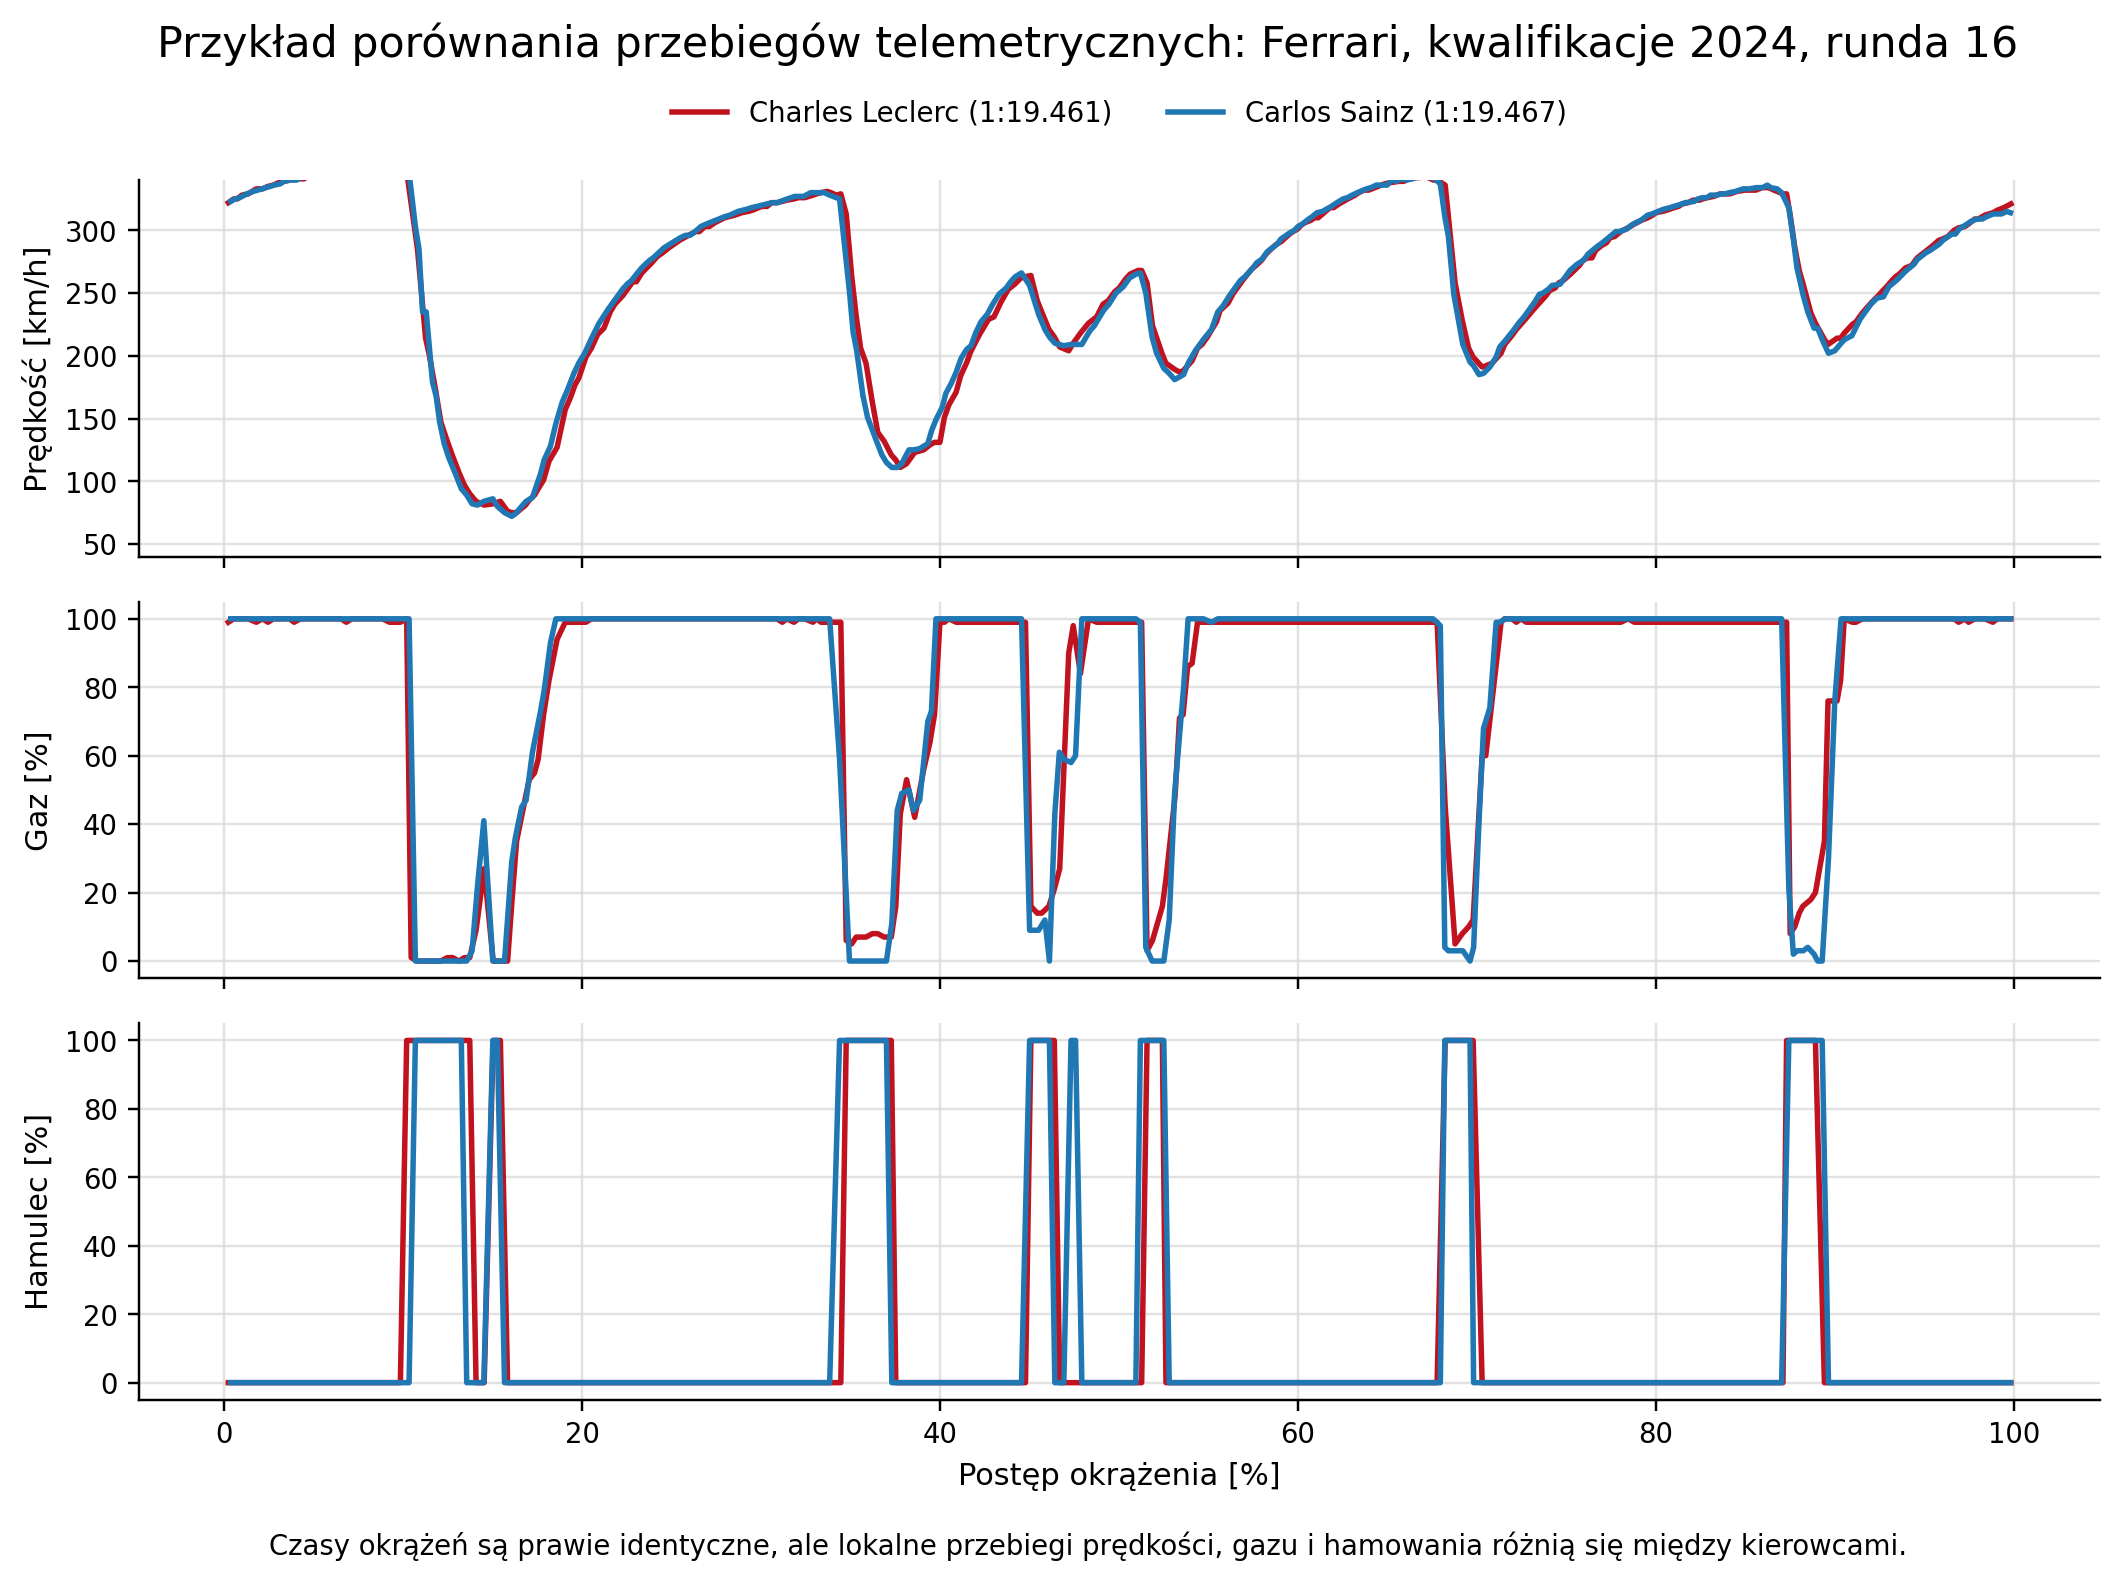
\includegraphics[width=0.9\textwidth]{figures/thesis/telemetry_overlay_lec_sai_2024_r16.png}
    \caption{Przykład porównania przebiegów telemetrycznych dla dwóch kierowców z bardzo podobnym czasem okrążenia.}
    \label{fig:telemetry_overlay_example}
\end{figure}
\FloatBarrier

Na wykresie różnice między kierowcami mają przede wszystkim charakter lokalny. W wielu fragmentach przebiegi prawie się pokrywają, ale w wybranych częściach okrążenia pojawiają się przesunięcia w momencie hamowania, zejścia z gazu i ponownego otwarcia przepustnicy. Przykładowo w środkowej części okrążenia jeden z kierowców wcześniej stabilizuje gaz po fazie hamowania, podczas gdy drugi dłużej utrzymuje częściowe otwarcie przepustnicy. Podobne różnice widać przy końcowych strefach hamowania, gdzie niewielkie przesunięcia czasowe przekładają się na inny przebieg prędkości. Sam czas okrążenia nie opisuje więc w pełni sposobu jazdy. Dwa bardzo podobne rezultaty mogą być zbudowane z nieco innych decyzji dotyczących hamowania, gazu i utrzymywania prędkości.

Zakres publicznie dostępnej telemetrii nakłada istotne ograniczenia interpretacyjne. W danych brakuje części informacji, które byłyby bardzo cenne przy pełniejszym opisie zachowania samochodu, między innymi kąta skrętu kierownicy, sił działających na pedały, ustawień samochodu, danych z zawieszenia, dokładnych map silnika czy szczegółowych parametrów aerodynamicznych. Ogranicza to możliwość jednoznacznego wyjaśnienia wszystkich przyczyn obserwowanych różnic między kierowcami. Dostępny zakres danych nadal pozwala jednak analizować przebieg okrążenia, porównywać decyzje dotyczące hamowania i przyspieszania oraz sprawdzać, czy w tych przebiegach pojawiają się powtarzalne wzorce charakterystyczne dla kierowców.

\section{Styl jazdy i identyfikacja kierowcy w literaturze}

Pojęcie stylu jazdy można rozumieć jako powtarzalny sposób prowadzenia pojazdu, widoczny w decyzjach podejmowanych przez kierowcę w kolejnych fragmentach trasy. W kontekście danych telemetrycznych styl nie jest pojedynczą wartością, ale zbiorem wzorców pojawiających się w czasie: sposobem budowania prędkości, rozkładem faz hamowania i przyspieszania, stabilnością prowadzenia samochodu oraz konsekwencją podobnych decyzji w wielu przejazdach. Pozwala to potraktować styl jazdy jako problem analizy danych, a nie wyłącznie opis jakościowy.

W literaturze można znaleźć wiele prac pokazujących, że zachowanie kierowcy pozostawia mierzalny ślad w danych z pojazdu. Systemy rozpoznawania stylu jazdy i zachowania kierowców są opisywane między innymi w kontekście bezpieczeństwa, systemów wspomagania kierowcy, ubezpieczeń oraz personalizacji pojazdu \cite{driving_style_review}. Kluczowa jest tutaj sama idea: jeżeli sposób prowadzenia pojazdu jest powtarzalny, to część tej powtarzalności powinna być widoczna w danych.

W pracach dotyczących identyfikacji kierowcy często wykorzystuje się dane z czujników samochodu, magistrali CAN-BUS lub systemów OBD-II. Klasyfikacja osoby prowadzącej pojazd może być oparta na sygnałach rejestrowanych przez samochód \cite{driver_can_identification}, a w wybranych podejściach nawet na danych z pojedynczego zakrętu \cite{hallac2016}. Jest to szczególnie bliskie tematyce tej pracy, ponieważ zakręt koncentruje wiele decyzji kierowcy w krótkim czasie: hamowanie, redukcję biegu, utrzymanie prędkości minimalnej i powrót na gaz.

Inny przykład stanowią badania oparte na danych telematycznych z normalnej jazdy drogowej, gdzie identyfikacja kierowcy może być łączona z analizą ważności cech, na przykład przy użyciu modelu Random Forest \cite{wang2017}. Podobne założenie przyjęto w części interpretowalnej: modele oparte na ręcznie zdefiniowanych cechach służą nie tylko do rozpoznania kierowcy, ale także do wskazania, które cechy najmocniej wpływają na decyzję modelu.

Nowsze podejścia coraz częściej wykorzystują reprezentacje ukryte i głębokie uczenie. Przykładem jest Driver2vec \cite{driver2vec}, czyli model tworzący embedding stylu jazdy na podstawie krótkiego fragmentu danych. Styl kierowcy można więc traktować nie tylko jako zestaw ręcznie wybranych cech, ale również jako reprezentację wydobytą automatycznie z przebiegu sygnałów. Podobną logikę wykorzystują modele sekwencyjne i hybrydowe zastosowane w eksperymentach.

W kontekście Formuły 1 dostępnych prac naukowych jest mniej niż w obszarze klasycznej telematyki drogowej. Publiczne dane F1 są bogate, ale nadal ograniczone względem danych zespołowych. Pojawiają się jednak prace i projekty analizujące trajektorie telemetryczne, klasteryzację oraz identyfikację kierowcy na podstawie fragmentów zakrętów \cite{f1_fda_thesis,withseismic2026}. Temat jest więc aktualny, ale nadal pozostawia miejsce na własną analizę porównującą modele tabularne, sekwencyjne i hybrydowe oraz badającą wpływ zespołu na wyniki klasyfikacji.

Na tle tych prac analiza łączy kilka elementów: publiczne dane Formuły 1, pełny proces od audytu danych po modele klasyfikacyjne oraz porównanie trzech setupów badawczych. Oprócz samej skuteczności klasyfikacji uwzględniono interpretowalność wyników oraz wpływ zespołu i samochodu na rozpoznawany profil telemetryczny.

\section{Klasyfikacja nadzorowana}

Problem rozpoznawania kierowcy sformułowano jako wieloklasową klasyfikację nadzorowaną. W takim zadaniu dla każdej próbki znana jest etykieta, a model uczy się odwzorowania między wejściem a klasą. Za etykietę przyjęto kierowcę, a wejściem był albo wektor cech opisujących całe okrążenie, albo sekwencja telemetryczna.

Najważniejszym problemem w klasyfikacji nie jest samo dopasowanie modelu do danych treningowych, lecz generalizacja. Model powinien działać na danych, których nie widział podczas uczenia. Jeżeli osiąga bardzo dobry wynik na treningu, ale słaby na walidacji lub teście, oznacza to przeuczenie. W analizowanym zbiorze szczególnie ważne było podobieństwo okrążeń z tej samej sesji, dlatego zastosowano walidację grupowaną po sesjach.

\section{Regresja logistyczna}

Regresja logistyczna jest jednym z podstawowych modeli klasyfikacyjnych. Pomimo nazwy, w tym zastosowaniu nie służy do przewidywania wartości ciągłej, lecz do estymacji prawdopodobieństwa przynależności próbki do danej klasy \cite{bishop2006}. Model najpierw tworzy liniową kombinację cech, a następnie przekształca ją do przedziału od 0 do 1 za pomocą funkcji logistycznej.

Dla przypadku binarnego funkcję logistyczną można zapisać jako:

\[
\sigma(z) = \frac{1}{1 + e^{-z}},
\]

gdzie \(z\) jest wynikiem liniowym modelu. W klasyfikacji wieloklasowej stosuje się analogiczne podejście z funkcją softmax, która zwraca rozkład prawdopodobieństwa po klasach.

\begin{figure}[H]
\centering
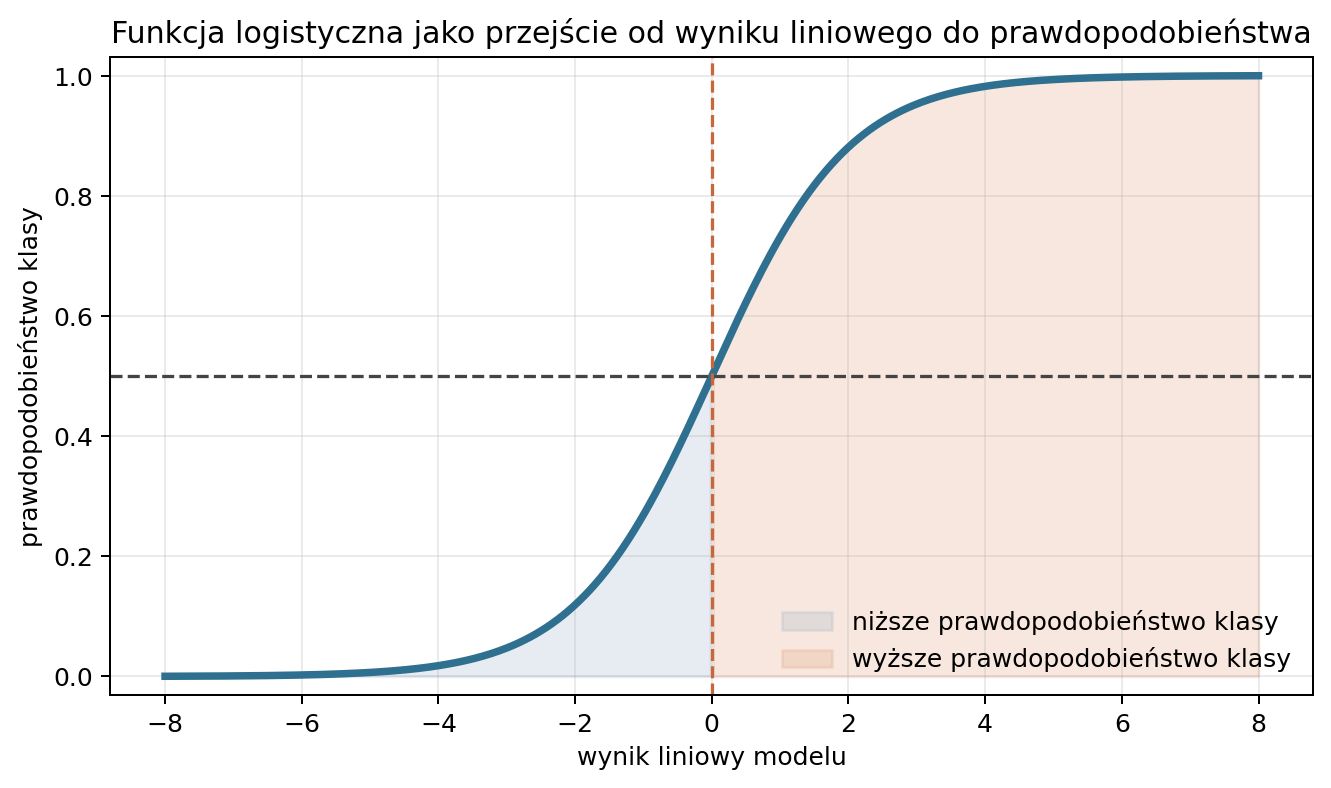
\includegraphics[width=0.64\textwidth]{30_theory_logistic_sigmoid.png}
\caption{Funkcja logistyczna jako przejście od wyniku liniowego do prawdopodobieństwa.}
\label{fig:theory-logistic}
\end{figure}
\FloatBarrier

Regresja logistyczna pełni rolę modelu interpretowalnego. Umożliwia nie tylko klasyfikację, lecz także analizę cech na podstawie wartości współczynników. Jeżeli dana cecha ma duży współczynnik dla konkretnej klasy, jej większa wartość zwiększa prawdopodobieństwo przypisania próbki do tej klasy. Współczynniki nie są jednak automatycznie dowodem przyczynowości; pełnią raczej funkcję wskazówki, które cechy telemetryczne model uznał za przydatne.

W modelach liniowych ważna jest regularyzacja. Regularyzacja L2 ogranicza zbyt duże wartości współczynników, a regularyzacja L1 może dodatkowo prowadzić do wyzerowania części z nich. Jest to użyteczne, gdy liczba cech jest duża, a nam zależy na prostszym i bardziej stabilnym modelu.

\section{Modele drzewiaste i boostingowe}

Modele drzewiaste dzielą przestrzeń cech na prostsze obszary decyzyjne. Pojedyncze drzewo decyzyjne jest łatwe do zrozumienia, ale może łatwo dopasować się zbyt mocno do danych treningowych. Random Forest ogranicza ten problem przez budowę wielu drzew na losowych podzbiorach danych i cech, a następnie agregację ich predykcji \cite{breiman2001}.

Modele boostingowe działają inaczej: budują kolejne słabsze modele tak, aby poprawiały błędy poprzednich. Często osiągają bardzo dobre wyniki na danych tabularnych, ale wymagają kontroli przeuczenia. Random Forest, HistGradientBoosting oraz XGBoost potraktowano jako modele porównawcze dla podejść liniowych i sekwencyjnych.

Różnicę między podejściem typu Random Forest a boostingiem przedstawiono schematycznie na rysunku~\ref{fig:theory-tree-boosting}. W pierwszym przypadku wiele drzew powstaje równolegle, a wynik jest agregowany. W drugim kolejne drzewa są dodawane sekwencyjnie i skupiają się na poprawianiu błędów wcześniejszych modeli.

\begin{figure}[H]
\centering
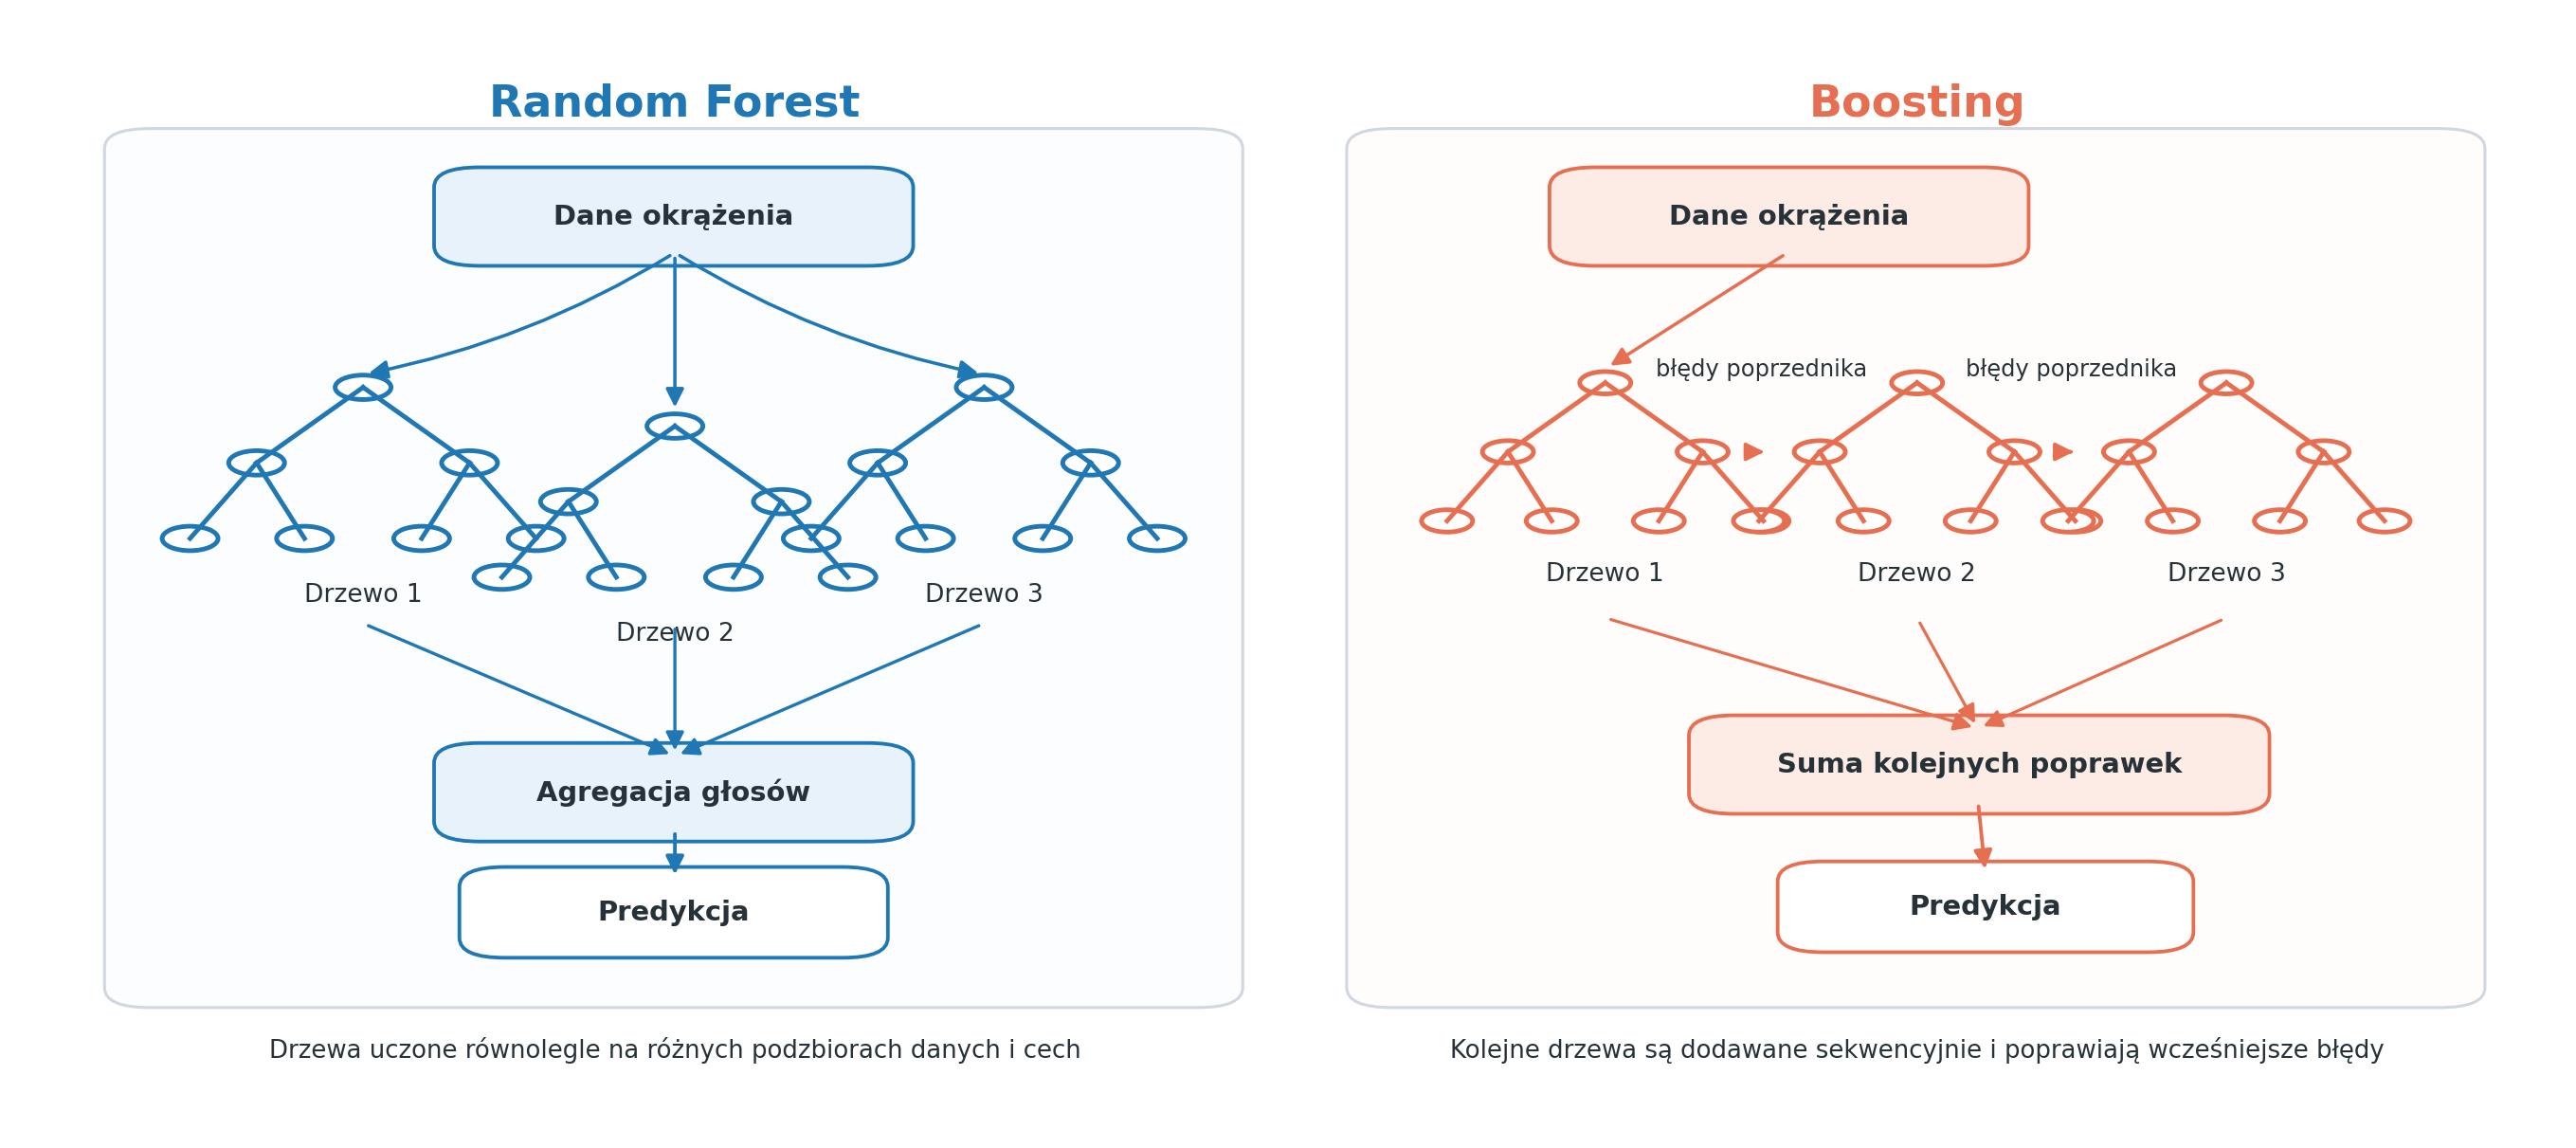
\includegraphics[width=0.98\textwidth,height=0.30\textheight,keepaspectratio=false]{33_theory_tree_boosting_concept.png}
\caption{Schematyczne porównanie idei Random Forest i modeli boostingowych.}
\label{fig:theory-tree-boosting}
\end{figure}
\FloatBarrier

\section{Modele sekwencyjne i CNN 1D}

Okrążenie Formuły 1 można opisać nie tylko jako zestaw statystyk, ale też jako sekwencję wartości telemetrycznych. W takim podejściu model dostaje przebieg sygnałów w czasie: prędkość, gaz, hamowanie, obroty i bieg. Żeby sekwencje mogły być użyte w sieci neuronowej, zostały przeskalowane do tej samej długości.

Sieć konwolucyjna 1D (\texttt{1D CNN}) przesuwa filtry po osi czasu i szuka lokalnych wzorców. W przypadku telemetrii takim wzorcem może być fragment hamowania, przejście z hamowania do gazu, stabilizacja prędkości albo seria zmian biegów. Klasyczne sieci konwolucyjne są znane głównie z analizy obrazów, ale idea lokalnego filtra może być stosowana również do sygnałów jednowymiarowych \cite{lecun1998}.

\begin{figure}[H]
\centering
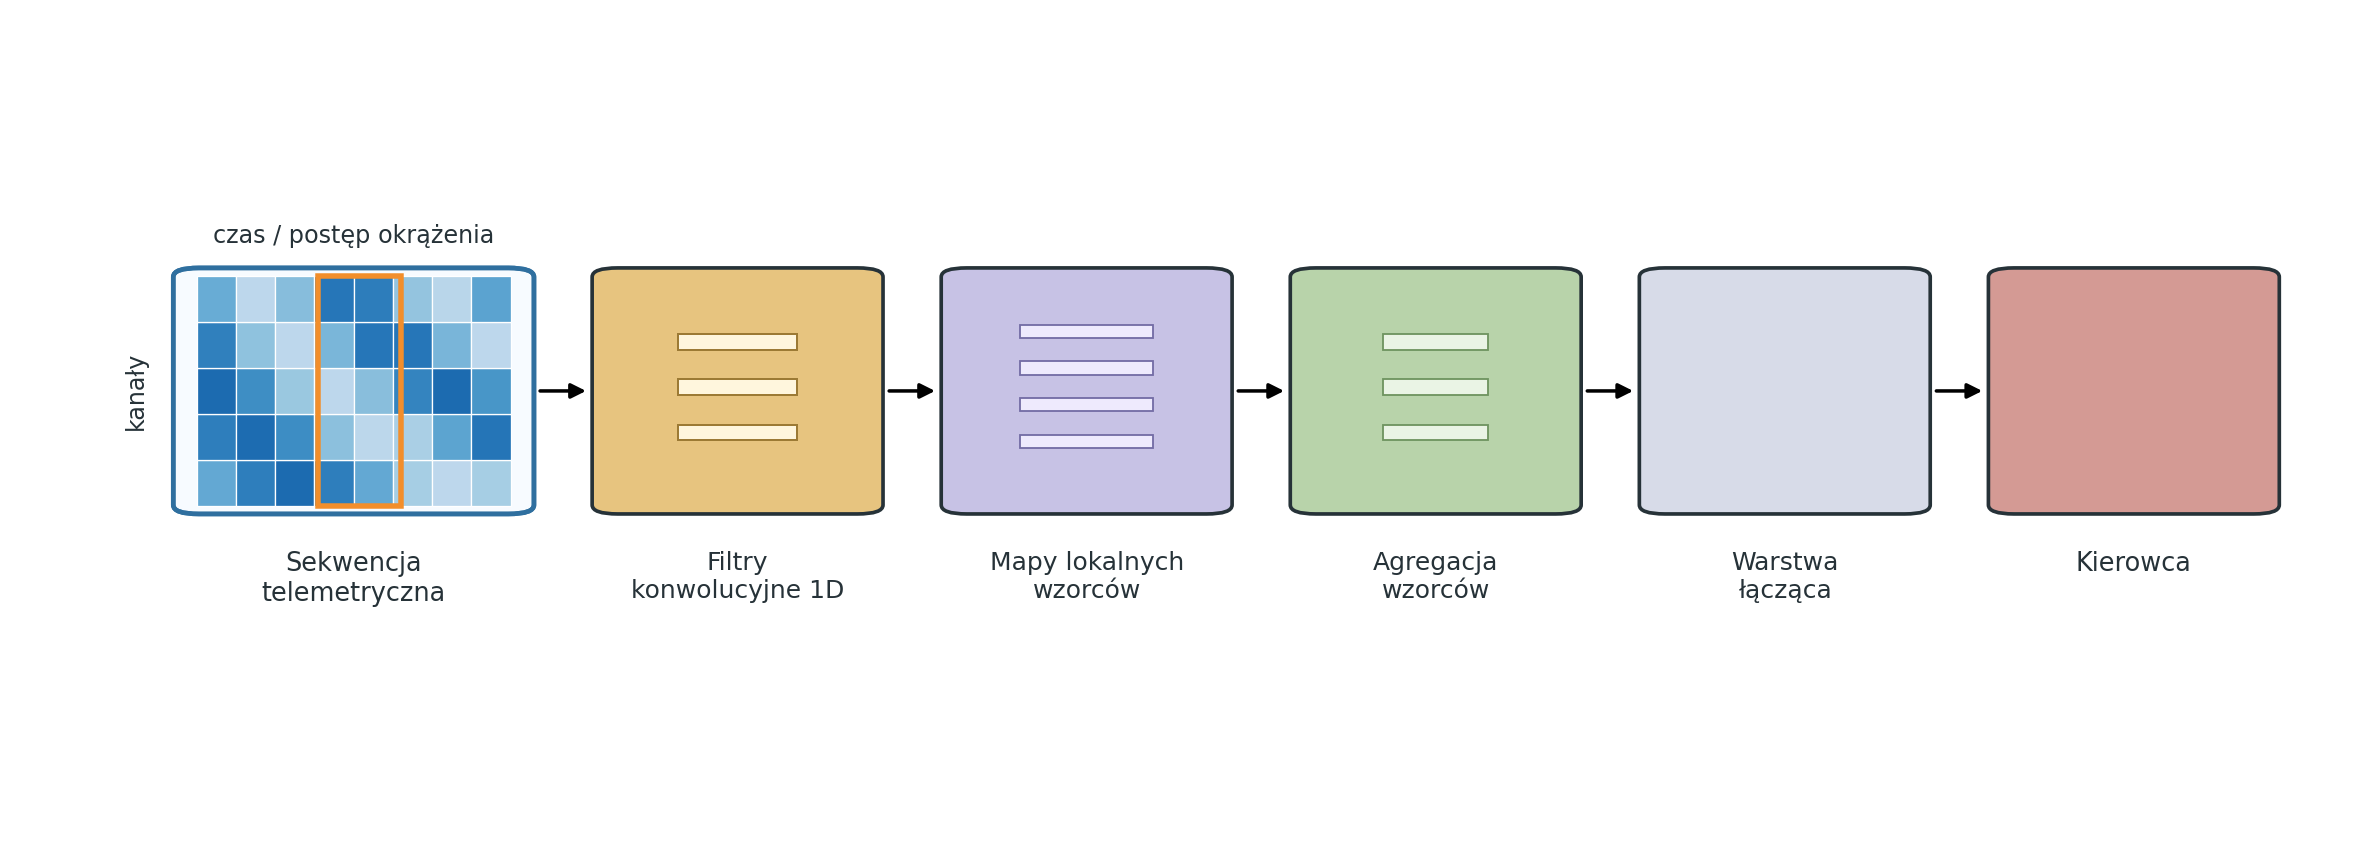
\includegraphics[width=\textwidth]{31_theory_1d_cnn_concept.png}
\caption{Schemat działania modelu CNN 1D dla sekwencji telemetrycznej.}
\label{fig:theory-cnn}
\end{figure}
\FloatBarrier

\texttt{CNN} dobrze pasuje do tego problemu, ponieważ styl jazdy może ujawniać się w krótkich fragmentach okrążenia. Model nie musi znać ręcznie opisanych zakrętów, aby wykrywać powtarzalne lokalne wzorce w przebiegu sygnałów.

\section{GRU, LSTM i model hybrydowy}

Modele rekurencyjne analizują sekwencję krok po kroku, przenosząc informację o wcześniejszych elementach sygnału. Klasyczne sieci rekurencyjne mają jednak problem z uczeniem długich zależności, dlatego opracowano architektury z bramkami, takie jak \texttt{LSTM} i \texttt{GRU}. \texttt{LSTM} wykorzystuje mechanizm komórki pamięci i bramek, aby łatwiej przechowywać informacje przez dłuższy czas \cite{hochreiter1997}. \texttt{GRU} jest uproszczoną architekturą bramkową również zaprojektowaną do pracy z sekwencjami \cite{cho2014}.

W analizowanym problemie sprawdzono \texttt{GRU} i \texttt{LSTM}, ponieważ okrążenie jest naturalnie uporządkowanym przebiegiem czasowym. Są to architektury stanowiące naturalny punkt porównania dla \texttt{CNN}: modele rekurencyjne lepiej akcentują zależności rozwijające się w czasie, a konwolucyjne dobrze obrazują lokalne wzorce w krótszych fragmentach sekwencji.

Ostatnim wariantem był model hybrydowy. Łączy on reprezentację sekwencyjną z cechami tabularnymi. Taki model może jednocześnie korzystać z lokalnych wzorców telemetrii oraz z syntetycznych informacji o całym okrążeniu, np. średniej prędkości, udziału pełnego gazu czy liczby zmian biegów.

\section{Walidacja i metryki}

W klasyfikacji najprostszy podział na trening i test może prowadzić do zbyt optymistycznych wyników, szczególnie gdy próbki są naturalnie pogrupowane. Grupą przyjętą w walidacji była sesja. Okrążenia z jednej sesji mają ten sam tor, warunki i podobny kontekst, dlatego nie powinny trafiać jednocześnie do treningu i testu.

Główną metodą walidacji był \texttt{StratifiedGroupKFold}, czyli wariant walidacji krzyżowej łączący zachowanie podobnych proporcji klas w foldach z rozdzieleniem grup między trening i test \cite{sklearn_sgkf}.

\begin{figure}[H]
\centering
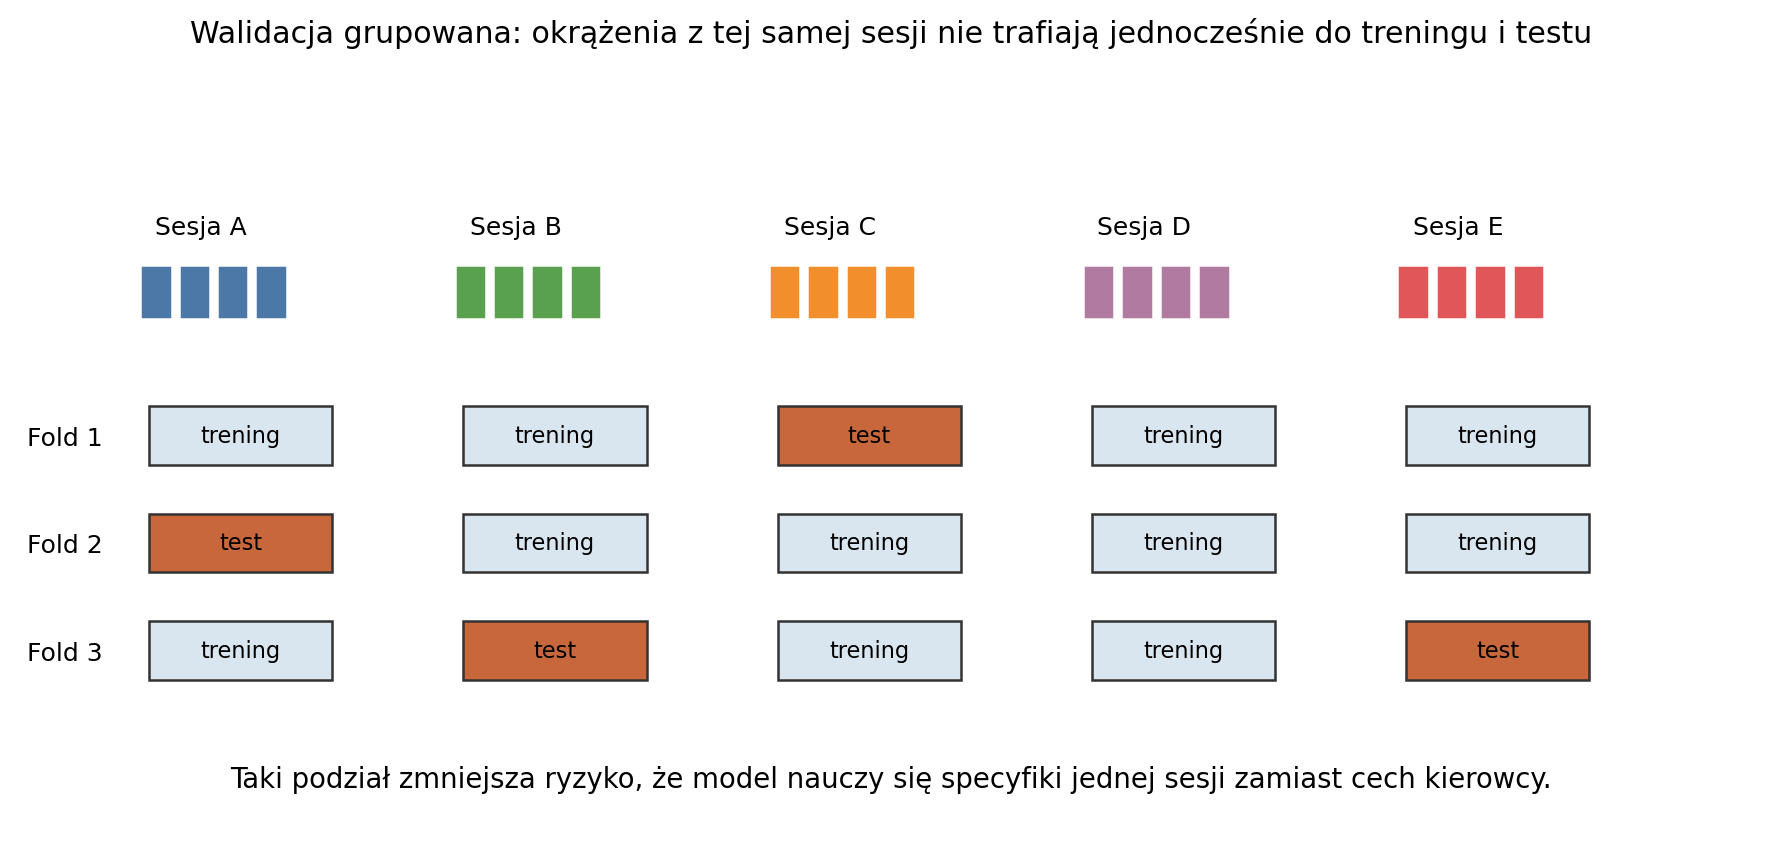
\includegraphics[width=0.90\textwidth]{32_theory_grouped_cv.png}
\caption{Schemat walidacji grupowanej po sesjach.}
\label{fig:theory-grouped-cv}
\end{figure}
\FloatBarrier

Do oceny modeli użyto kilku metryk. Accuracy oznacza udział poprawnych predykcji:

\[
Accuracy = \frac{\text{liczba poprawnych predykcji}}{\text{liczba wszystkich predykcji}}.
\]

Sama accuracy może jednak być myląca, jeżeli klasy są nierówno reprezentowane. Dlatego za główną metrykę przyjęto macro F1. Dla każdej klasy liczone są precision i recall, następnie F1:

\[
F1 = 2 \cdot \frac{precision \cdot recall}{precision + recall}.
\]

Macro F1 jest średnią wartości F1 po klasach. Metryka ta pozwala oceniać jakość modeli w problemach wieloklasowych bez nadmiernego faworyzowania najliczniejszych klas \cite{sokolova2009}. W analizie kierowców jest szczególnie użyteczna, ponieważ każda klasa ma podobne znaczenie w końcowym wyniku, niezależnie od liczby okrążeń danego kierowcy. Dodatkowo analizowano macierze pomyłek, które pokazują nie tylko ogólny wynik, ale też pary kierowców najczęściej mylone przez model.

\chapter{Dane i eksploracyjna analiza danych}

\section{Źródła danych}

Podstawowym źródłem danych była biblioteka \texttt{FastF1}. Jest to biblioteka Pythona przeznaczona do pobierania i analizy publicznie dostępnych danych Formuły 1. Jej najważniejszą zaletą w tym projekcie była możliwość połączenia kilku typów informacji w jednym procesie przetwarzania danych: czasów okrążeń, sektorów, informacji o oponach, wyników sesji, danych pogodowych, telemetrii samochodu, danych pozycyjnych oraz harmonogramu wydarzeń. Biblioteka udostępnia między innymi dane okrążeń, telemetrię samochodu, pozycję, dane opon, pogodę, harmonogram sesji oraz wyniki \cite{fastf1_docs}.

Najczęściej wykorzystywanym obiektem była sesja, np. kwalifikacje albo wyścig dla konkretnego Grand Prix. Po załadowaniu sesji można uzyskać tabelę okrążeń, wyniki, dane pogodowe oraz przebiegi telemetryczne dla wybranych kierowców i okrążeń. Tabela okrążeń zawierała między innymi kierowcę, numer okrążenia, czas okrążenia, czasy sektorów, mieszankę opon, wiek opon, status toru oraz informację o poprawności okrążenia. Dane telemetryczne obejmowały sygnały takie jak \texttt{Speed}, \texttt{Throttle}, \texttt{Brake}, \texttt{RPM}, \texttt{nGear}, \texttt{DRS}, a dane pozycyjne pozwalały uzyskać współrzędne \texttt{X}, \texttt{Y}, \texttt{Z}.

Biblioteka była szczególnie wygodna w tym projekcie, ponieważ umożliwiała przejście od poziomu sesji do poziomu pojedynczego okrążenia. Najpierw przeprowadzono audyt dostępności danych, potem odfiltrowano okrążenia według warunków i jakości, a dopiero na końcu pobierano telemetrię dla wybranych próbek. Było to istotne ze względów praktycznych: pobieranie pełnej telemetrii dla wszystkich okrążeń jest dużo bardziej czasochłonne niż praca na tabelach okrążeń.

\texttt{FastF1} korzysta z danych pobieranych z zewnętrznych źródeł, dlatego istotne było użycie lokalnego cache. Pozostawienie cache włączonego przyspiesza ponowne uruchamianie skryptów i pomaga uniknąć przekraczania limitów serwerów API \cite{fastf1_docs}. Pierwsze pobranie sesji mogło trwać długo, ale kolejne uruchomienia korzystały już z danych zapisanych lokalnie. Przy pobieraniu wielu sezonów ograniczało to czas działania skryptów i liczbę ponownych zapytań do tych samych endpointów.

Zakres danych udostępnianych przez \texttt{FastF1} jest węższy niż zakres danych inżynierskich dostępnych zespołom Formuły 1. Ogranicza to możliwość pełnego wyjaśniania przyczyn obserwowanych różnic, ale nadal pozwala badać te elementy stylu jazdy, które są widoczne w publicznym przebiegu okrążenia.

Pomocniczo rozważano również źródła takie jak Jolpica oraz OpenF1. Jolpica jest istotna przede wszystkim jako źródło metadanych i następca Ergast API w ekosystemie \texttt{FastF1} \cite{fastf1_docs}. OpenF1 może być natomiast użyteczne jako dodatkowe źródło walidacji w przyszłości. W obecnym etapie głównym źródłem danych pozostało jednak \texttt{FastF1}, aby zachować spójność całego procesu pobierania, filtrowania i ekstrakcji telemetrii.

\section{Zakres danych}

W projekcie przygotowano trzy główne setupy eksperymentalne przedstawione w tabeli~\ref{tab:setups}. Zbiory różnią się nie tylko liczbą okrążeń, ale też poziomem czystości danych i trudnością zadania. Kwalifikacje 2023--2025 są najmniejszym i najczystszym punktem startowym. Kwalifikacje 2018--2025 sprawdzają, czy wniosek utrzymuje się w dłuższym horyzoncie czasowym. Czyste okrążenia wyścigowe 2025 zwiększają liczbę próbek, ale wprowadzają większą zmienność wynikającą z opon, paliwa, stintu i kontekstu wyścigowego.

\begin{table}[H]
\centering
\small
\begin{tabular}{l c l r}
\toprule
Setup & Zakres lat & Kierowcy & Liczba okrążeń \\
\midrule
Kwalifikacje, krótki horyzont & 2023--2025 & ALB, SAI, VER, OCO, LEC & 273 \\
Kwalifikacje, długi horyzont & 2018--2025 & SAI, VER, LEC, OCO, HAM & 698 \\
Wyścigi, czyste okrążenia & 2025 & SAI, VER, LEC, OCO, HAM & 4334 \\
\bottomrule
\end{tabular}
\caption{Główne setupy eksperymentalne.}
\label{tab:setups}
\end{table}

\begin{figure}[H]
\centering
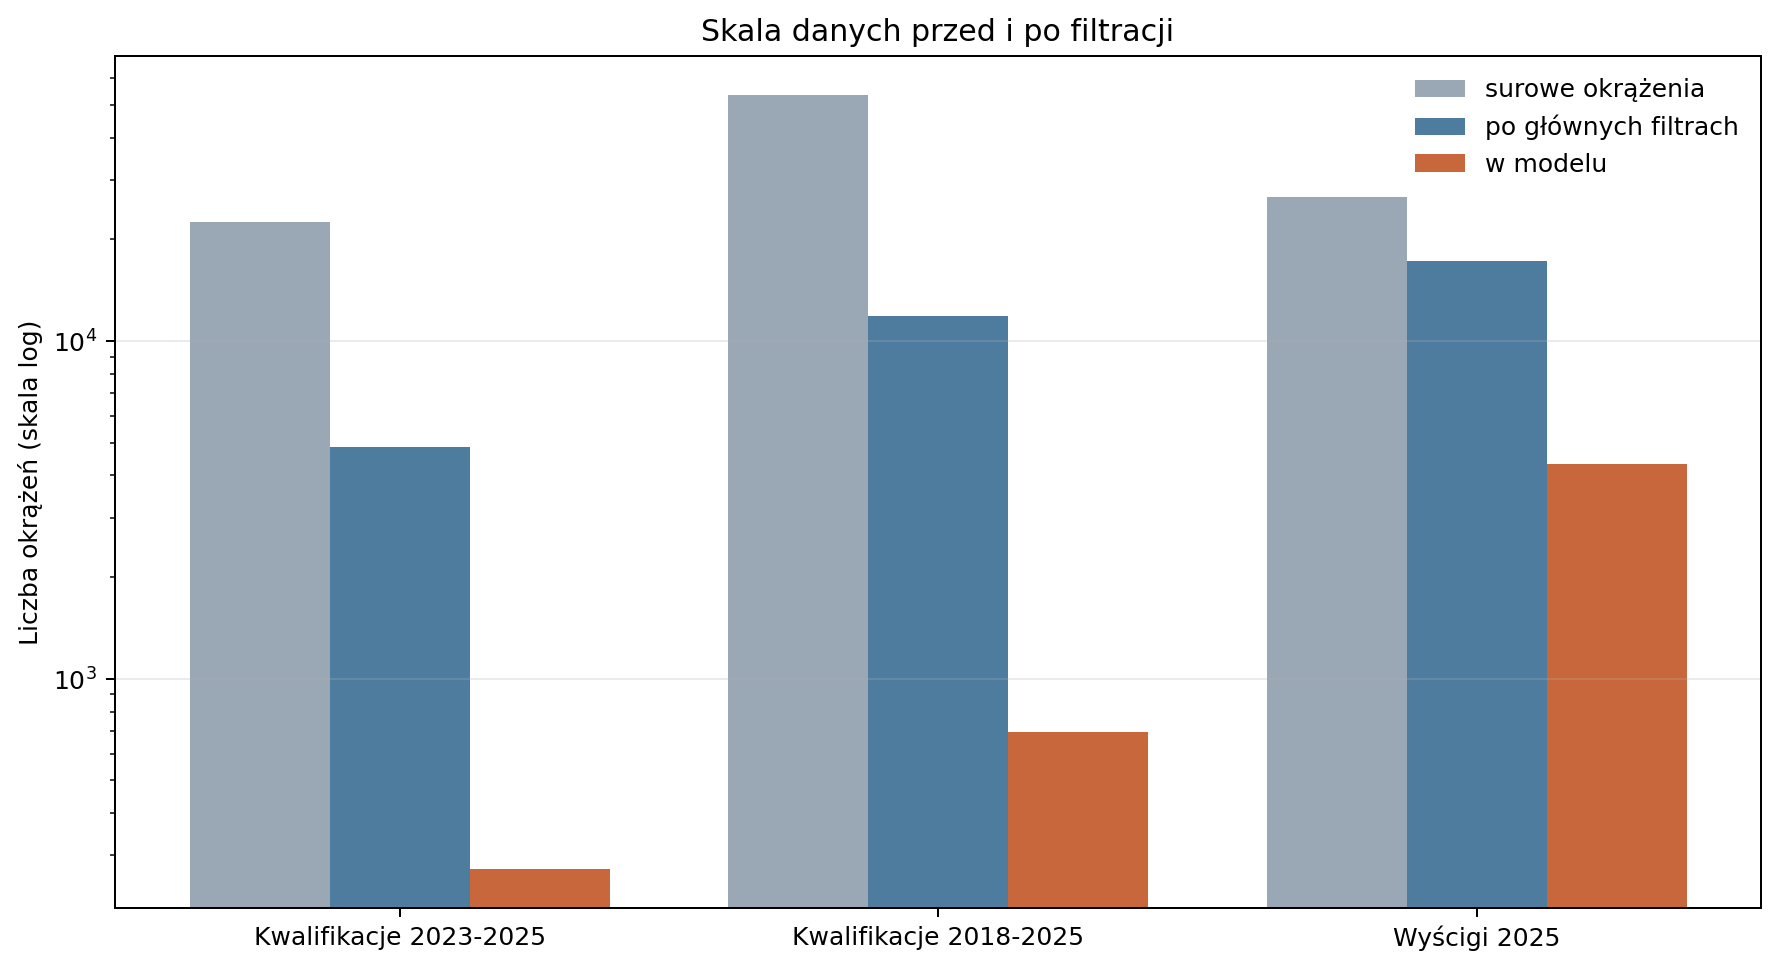
\includegraphics[width=0.95\textwidth]{24_eda_dataset_sizes.png}
\caption{Porównanie liczby okrążeń w danych surowych, po filtracji i w finalnych setupach modelowych.}
\label{fig:eda-dataset-sizes}
\end{figure}

\section{Redukcja danych}

Dane redukowano etapowo. Pozwalało to sprawdzić, które kryteria najmocniej zmniejszały zbiór oraz czy odrzucane były głównie okrążenia problematyczne z punktu widzenia modelowania stylu jazdy.

W kwalifikacjach 2023--2025 punkt startowy obejmował 22465 okrążeń. Po usunięciu okrążeń bez czasu, ograniczeniu do suchych sesji, filtrze poprawności, zielonym statusie toru i wyborze personal best pozostało 4853 okrążeń w czystym zbiorze pośrednim. Finalny setup pięciu kierowców zawierał 273 okrążenia.

W kwalifikacjach 2018--2025 punkt startowy obejmował 53690 okrążeń. Po analogicznych filtrach pozostało 11848 okrążeń personal best, a finalny setup pięciu kierowców zawierał 698 okrążeń.

W wyścigach 2025 punkt startowy obejmował 26692 okrążenia. Po usunięciu okrążeń bez czasu, mokrych sesji, okrążeń niedokładnych, neutralizacji, pit-in/pit-out oraz okrążeń odstających od lokalnej mediany stintu pozostało 17265 czystych okrążeń wyścigowych. Finalny setup pięciu kierowców zawierał 4334 okrążenia.

\section{Filtrowanie danych}

Dane były filtrowane etapowo. W kwalifikacjach uwzględniano między innymi: niepusty czas okrążenia, suche warunki, poprawność okrążenia, zielony status toru oraz wybór reprezentatywnego okrążenia kierowcy w sesji. W wyścigach dodatkowo odrzucano okrążenia pit-in/pit-out i okrążenia odstające od lokalnej mediany stintu.

\begin{figure}[H]
\centering
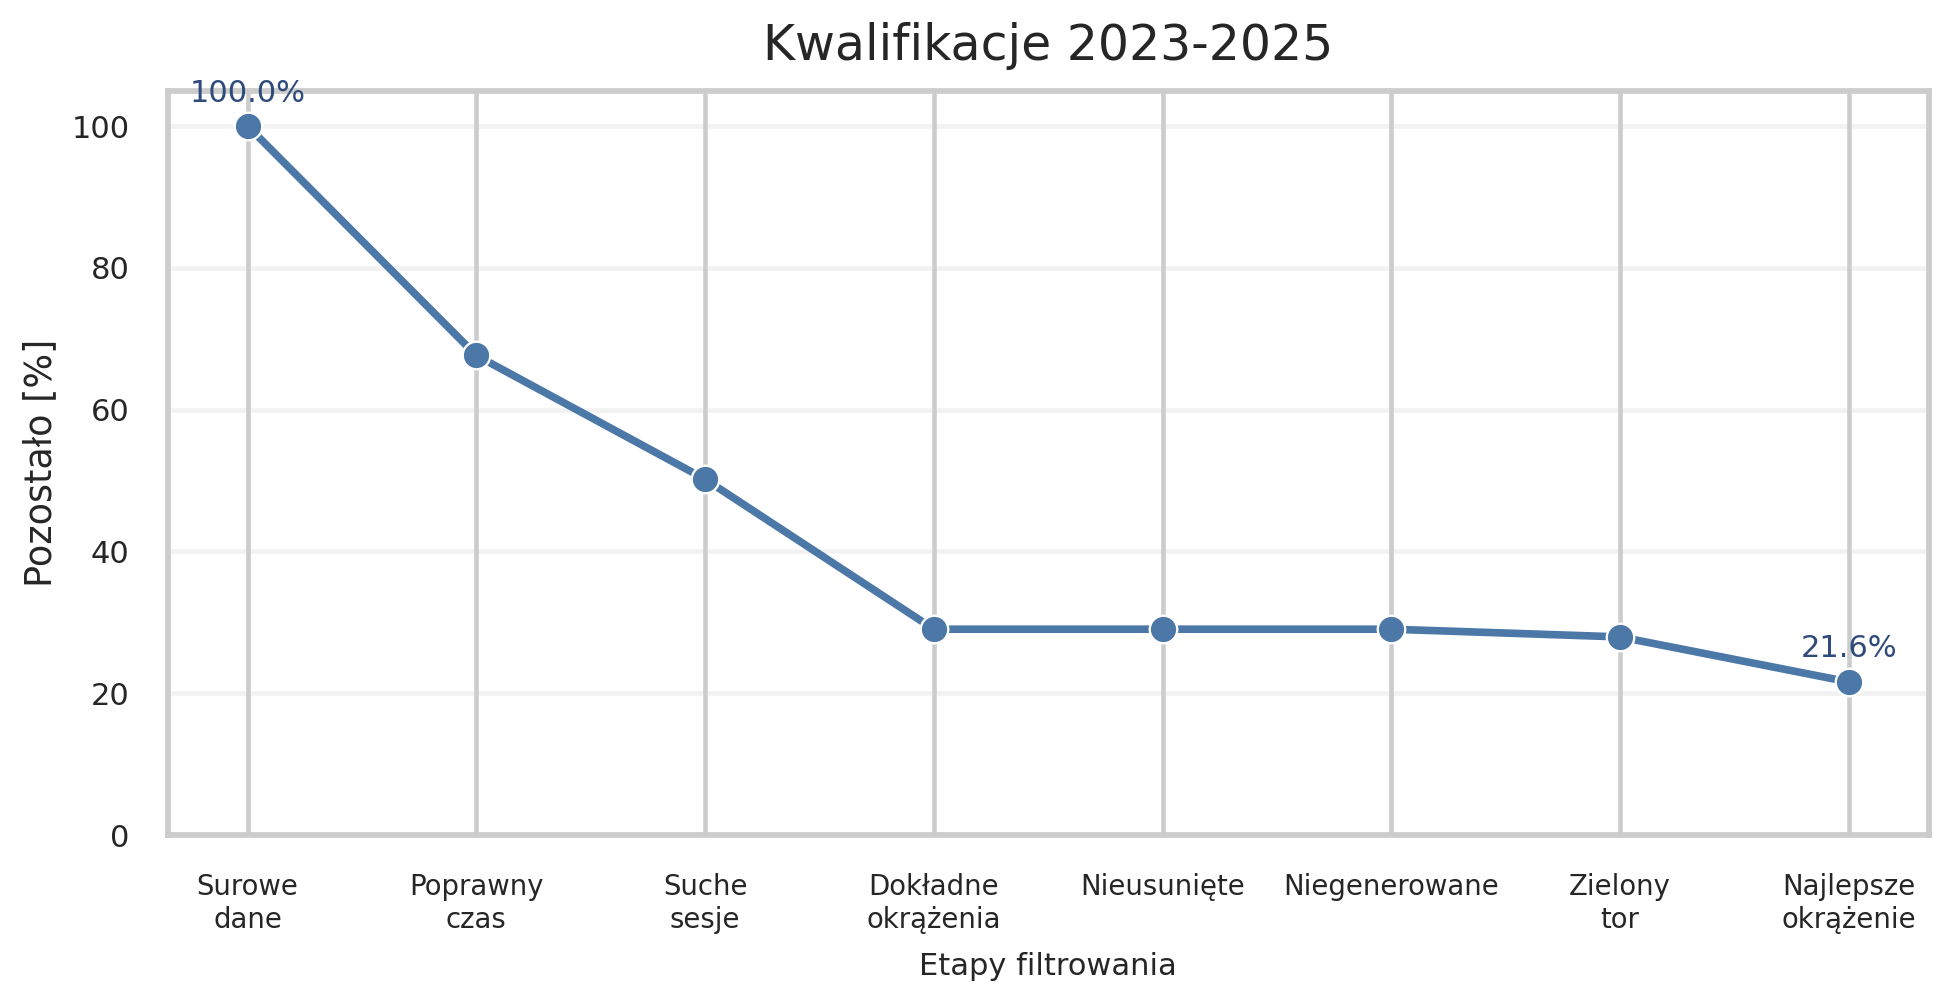
\includegraphics[width=0.92\textwidth]{01a_filter_funnel_qualifying_2023_2025.png}
\caption{Redukcja danych po kolejnych filtrach w setupie kwalifikacyjnym 2023--2025.}
\label{fig:filter-funnel-short-qualifying}
\end{figure}

\begin{figure}[H]
\centering
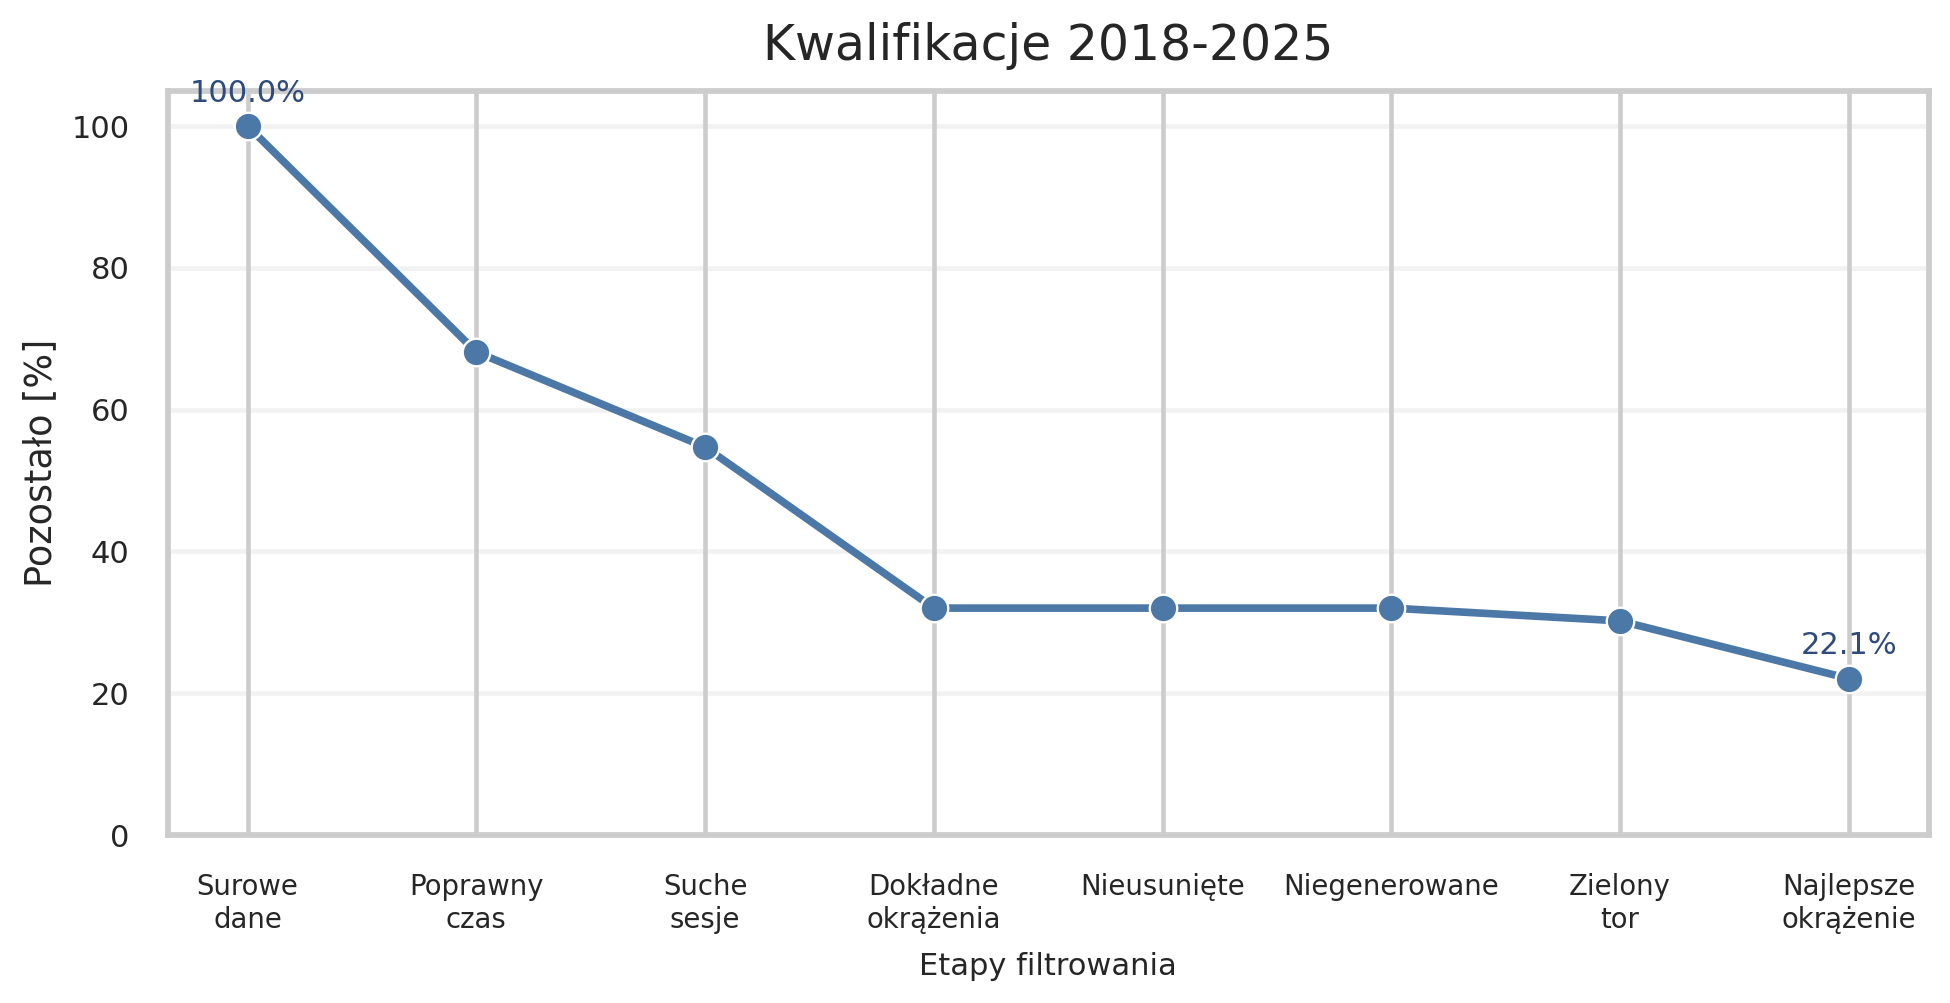
\includegraphics[width=0.92\textwidth]{01b_filter_funnel_qualifying_2018_2025.png}
\caption{Redukcja danych po kolejnych filtrach w setupie kwalifikacyjnym 2018--2025.}
\label{fig:filter-funnel-long-qualifying}
\end{figure}

\begin{figure}[H]
\centering
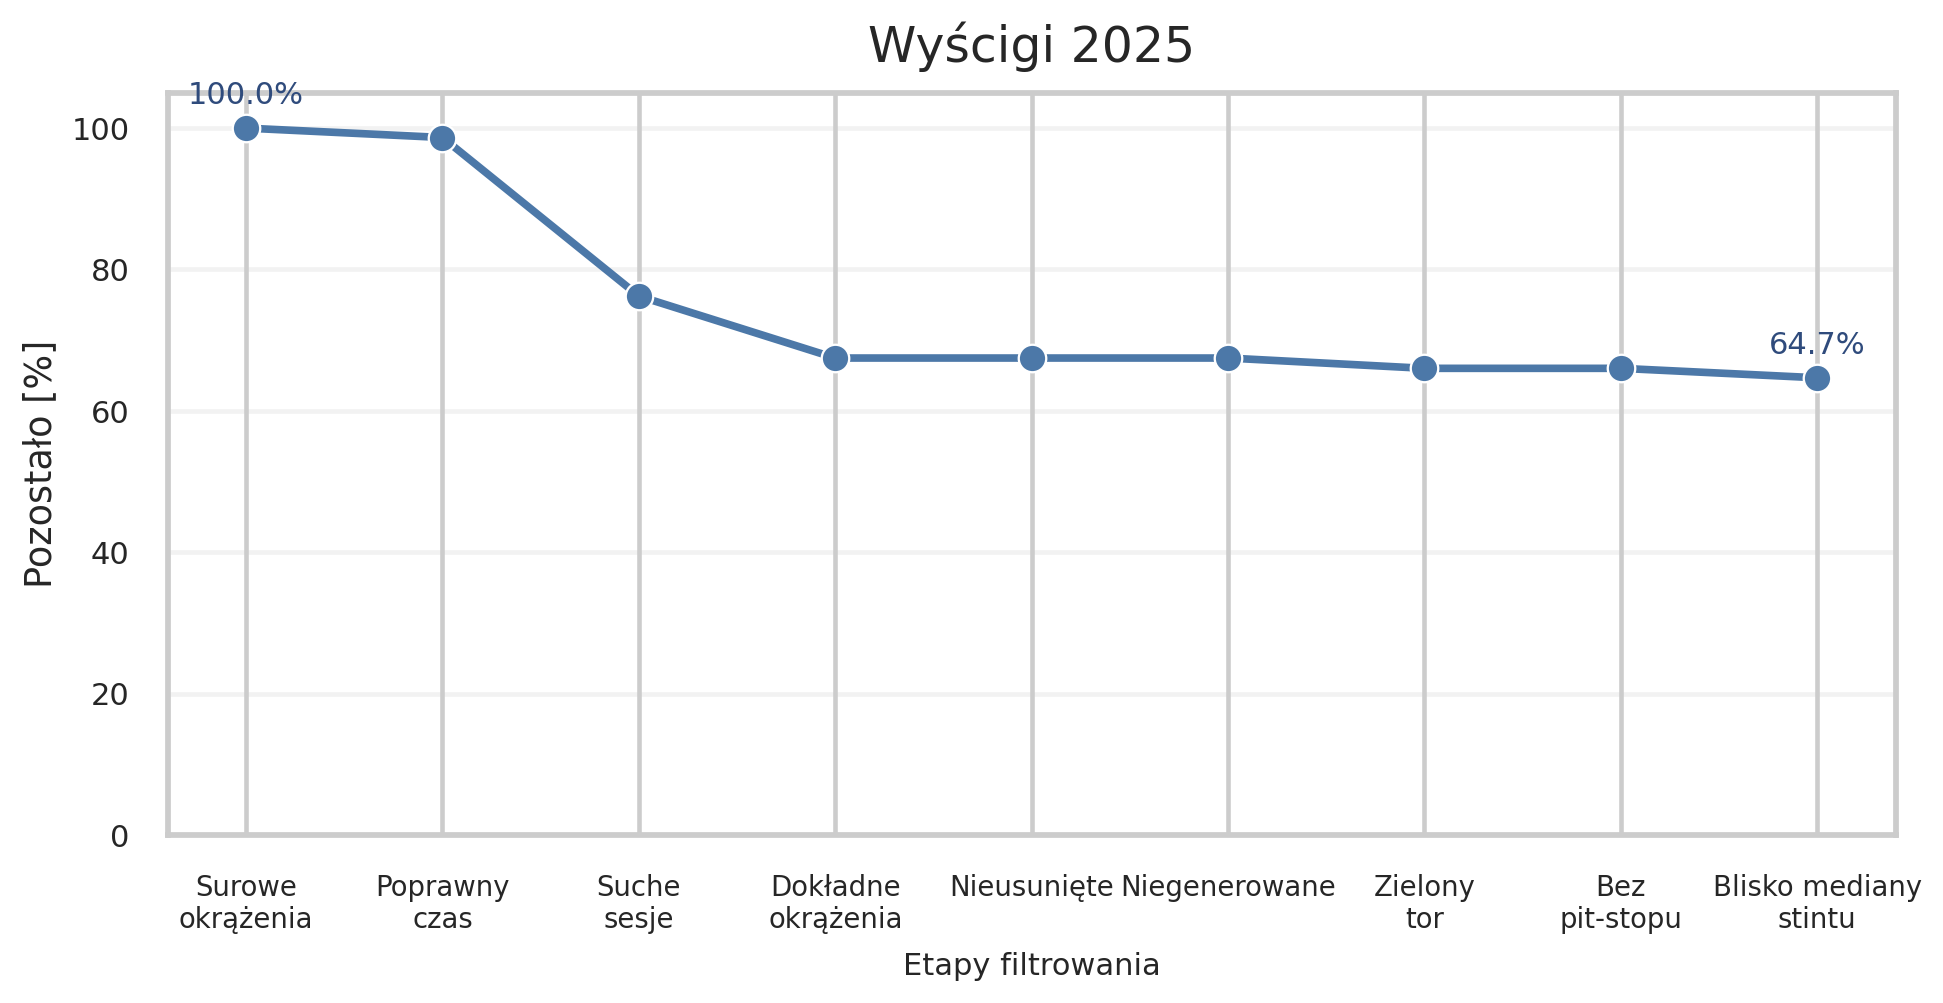
\includegraphics[width=0.92\textwidth]{01c_filter_funnel_race_2025.png}
\caption{Redukcja danych po kolejnych filtrach w setupie wyścigowym 2025.}
\label{fig:filter-funnel-race}
\end{figure}
\FloatBarrier

Największa redukcja w kwalifikacjach wynikała z trzech decyzji: odrzucenia okrążeń bez poprawnego czasu, ograniczenia danych do suchych sesji oraz wyboru najlepszych reprezentatywnych okrążeń kierowców. W setupach kwalifikacyjnych końcowy zbiór jest więc niewielki, ponieważ założeniem było ograniczenie powtarzalnych okrążeń z tej samej sesji i pozostawienie możliwie czystego sygnału.

W przypadku wyścigów redukcja wygląda inaczej. Po filtrach jakościowych nadal zostaje duża liczba okrążeń, ponieważ z jednej sesji wyścigowej można wykorzystać wiele czystych okrążeń tego samego kierowcy. Wynika to z innej definicji próbki: w kwalifikacjach wybierane jest głównie jedno reprezentatywne okrążenie, natomiast w wyścigu zachowywane są liczne okrążenia spełniające kryteria czystości.

\section{Wybór kierowców}

Wybór kierowców był istotnym elementem przygotowania eksperymentów. Zamiast analizować przypadkową grupę zawodników, zbudowano zbiór umożliwiający sensowne porównanie różnic stylu jazdy. Najpierw brano pod uwagę szeroki zbiór kierowców dostępnych w danych, a dopiero później zawężano analizę do grup, dla których liczba okrążeń, jakość danych i interpretowalność wyników pozwalały na stabilne modelowanie.

Pierwszym kryterium była liczba dostępnych okrążeń. Kierowcy z bardzo krótkim okresem startów, pojedynczymi zastępstwami lub małą liczbą czystych okrążeń nie są dobrymi kandydatami do modelowania, ponieważ model mógłby uczyć się przypadkowych cech kilku sesji zamiast powtarzalnego profilu jazdy. Dlatego w pierwszych eksperymentach zastosowano próg minimalnej liczby okrążeń, a w późniejszych setupach wybierano kierowców z możliwie dobrym pokryciem sezonów i sesji.

Drugim kryterium była sensowność porównania stylu jazdy. W Formule 1 styl kierowcy nie jest pojedynczą cechą, którą można bezpośrednio odczytać z jednego sygnału telemetrycznego. Jest raczej kombinacją kilku zachowań: sposobu wejścia w zakręt, preferencji balansu samochodu, pracy gazu, momentu rozpoczęcia hamowania, sposobu redukcji biegów, utrzymywania prędkości minimalnej oraz przyspieszania na wyjściu z zakrętu. Analizy branżowe Formuły 1 \cite{formula1_racing_id, autosport_driving_style} często opisują styl jazdy właśnie przez preferencję nadsterowności lub podsterowności, różnice w kształcie linii przejazdu oraz odmienny sposób zarządzania fazą hamowania i przyspieszania.

Takie opisy nie są traktowane jako dowód sam w sobie. Stanowią raczej punkt wyjścia do sformułowania problemu badawczego: jeżeli kierowcy faktycznie różnią się sposobem prowadzenia samochodu, to część tych różnic powinna być widoczna w telemetrii. Finalny wybór kierowców nie wynikał więc z założenia, że konkretna osoba musi mieć z góry przypisany styl. Dane miały sprawdzić, czy model potrafi odnaleźć powtarzalne wzorce i czy te wzorce da się później zinterpretować w kategoriach jazdy kierowcy.

Analiza była wykonywana także dla większej liczby zawodników, ale nie dla wszystkich kierowców sygnał był równie czytelny interpretacyjnie. Nie musi to oznaczać braku stylu jazdy; część kierowców może mieć mniej wyraźny profil w publicznej telemetrii, część może być silniej przykryta charakterystyką samochodu, a część może mieć po prostu zbyt mało danych. Bardziej wartościowe było pokazanie przypadków, w których klasyfikację da się stabilnie omówić, niż utrzymywanie wszystkich kierowców kosztem bardzo nierównych klas i słabszej interpretacji.

W krótkim setupie kwalifikacyjnym finalni kierowcy mieli po 54--55 okrążeń, więc klasy były praktycznie zbalansowane. W kwalifikacjach 2018--2025 wybrana piątka miała od 121 do 145 okrążeń, przy czym Ocon miał mniej danych niż pozostali, ale nadal wystarczająco dużo do modelowania. W setupie wyścigowym liczba próbek była dużo większa i mieściła się w zakresie 799--911 okrążeń na kierowcę.

Zawężenie listy kierowców potraktowano jako etap projektowania eksperymentu. Najpierw sprawdzono, czy w danych istnieje informacja pozwalająca rozpoznać kierowcę, a następnie skupiono się na grupach, w których tę informację można sensownie interpretować. Część badawcza przechodzi dzięki temu od pytania „czy model rozpoznaje kierowcę?” do ważniejszego pytania „jakie cechy telemetrii pozwalają go rozpoznać?”.

\section{Typy zmiennych i braki danych}

W danych występują identyfikatory okrążeń, kolumny kontekstowe, zmienne kategoryczne oraz numeryczne cechy modelowe. Większość cech wykorzystywanych przez modele ma charakter numeryczny, ponieważ powstaje przez agregację sygnałów telemetrycznych. Do modelowania nie wykorzystywano identyfikatorów takich jak \texttt{lap\_key}, etykiety \texttt{Driver} jako cechy wejściowej ani kolumn, które bezpośrednio identyfikowałyby próbkę.

Zmienne kategoryczne były traktowane ostrożnie. Część z nich, np. nazwa kierowcy, pełniła rolę etykiety, a nie wejścia modelu. Inne, takie jak \texttt{Team} lub kontekst sesji, mogły wprowadzać informację o samochodzie zamiast o samym kierowcy, dlatego były używane tylko w wybranych eksperymentach kontrolnych. Jeżeli zmienne kategoryczne były używane w modelach tabularnych, wymagały kodowania, natomiast w głównych wariantach interpretacyjnych nacisk położono na cechy numeryczne pochodzące z telemetrii.

Braki danych w numerycznych cechach modelowych były bardzo małe. W krótkim setupie kwalifikacyjnym pojedyncze braki dotyczyły głównie informacji o oponach, np. \texttt{TyreLife}. Zasadnicze sygnały telemetryczne i cechy zagregowane były kompletne. W długim setupie kwalifikacyjnym i w setupie wyścigowym najważniejsze cechy modelowe nie miały braków, więc nie stosowano złożonej strategii imputacji.

\section{Reprezentacja okrążenia}

Każde okrążenie było reprezentowane na dwa sposoby:

\begin{itemize}
    \item jako wektor ręcznie zdefiniowanych cech, np. średnia prędkość, udział pełnego gazu, liczba aktywacji hamulca, liczba zmian biegów;
    \item jako sekwencja telemetryczna z sygnałami \texttt{Speed}, \texttt{Throttle}, \texttt{Brake}, \texttt{RPM}, \texttt{nGear}.
\end{itemize}

\begin{figure}[H]
\centering
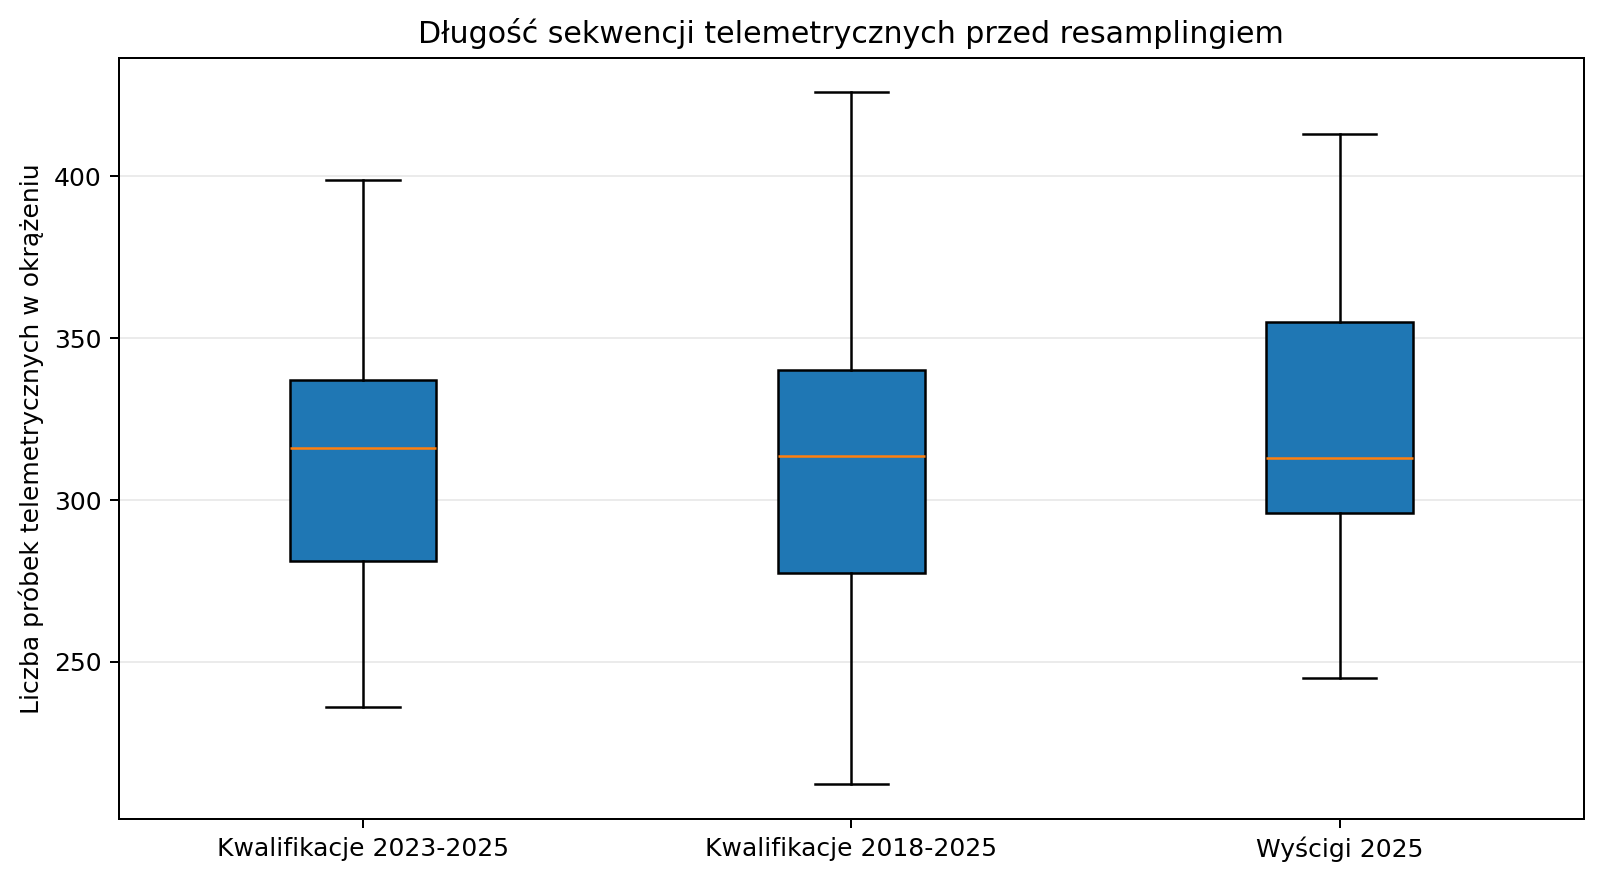
\includegraphics[width=0.90\textwidth]{27_eda_sequence_lengths.png}
\caption{Długość sekwencji telemetrycznych przed resamplingiem.}
\label{fig:eda-sequence-lengths}
\end{figure}

Sekwencje telemetryczne miały zmienną długość, dlatego przed treningiem modeli sekwencyjnych były resamplowane do stałej liczby próbek. Zmienność długości wynika z czasu okrążenia i sposobu próbkowania danych. Rozkład długości nie wskazywał jednak na problem uniemożliwiający uczenie modeli sekwencyjnych.

\section{Korelacje cech}

Przed modelowaniem warto sprawdzić, czy wybrane cechy opisują niezależne informacje, czy raczej różne ujęcia tego samego zjawiska. W danych telemetrycznych silna korelacja części cech jest oczekiwana, ponieważ prędkość, biegi, obroty silnika i praca przepustnicy są ze sobą fizycznie powiązane.

\begin{figure}[H]
\centering
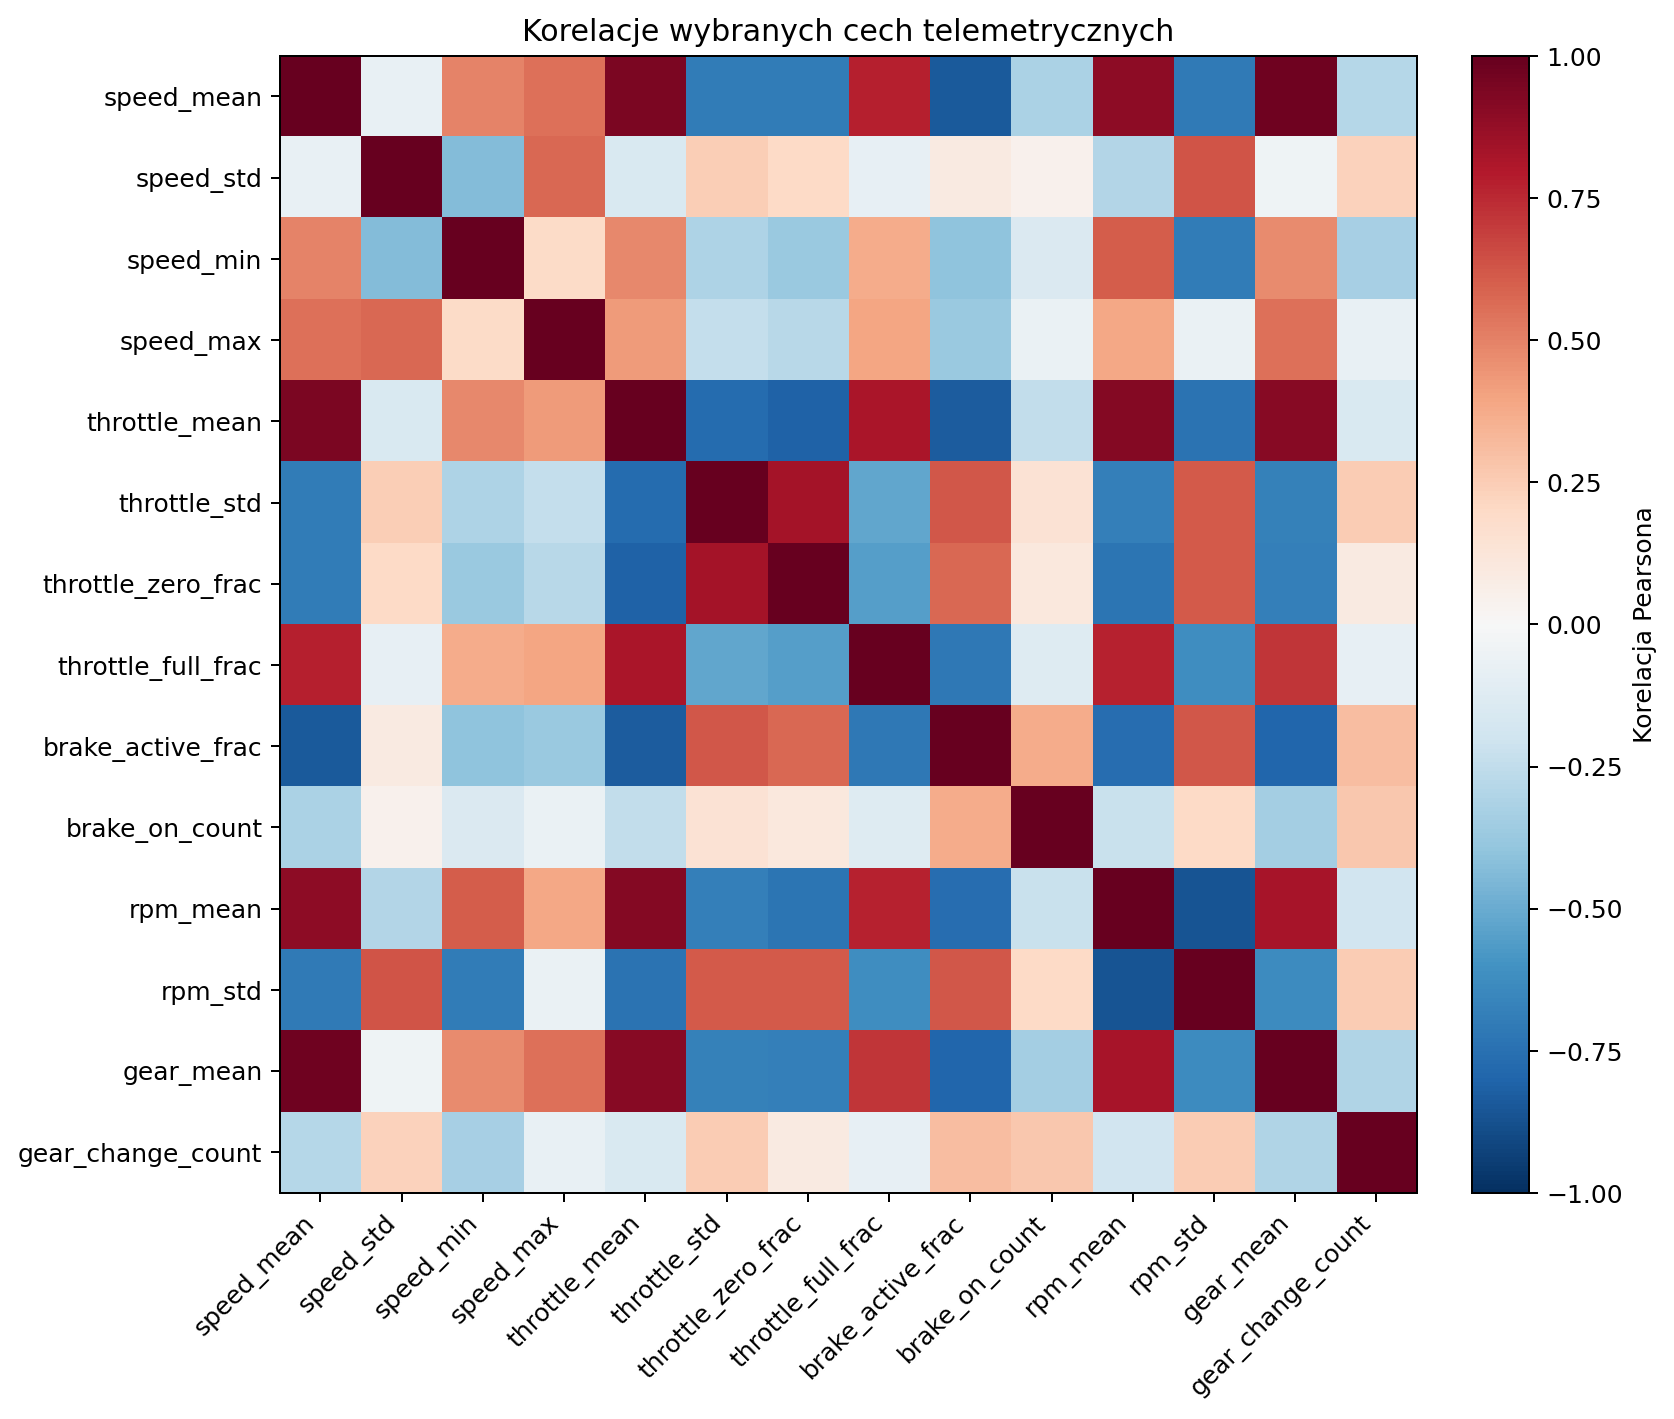
\includegraphics[width=0.90\textwidth]{29_eda_feature_correlation_heatmap.png}
\caption{Korelacje wybranych cech telemetrycznych.}
\label{fig:eda-correlation}
\end{figure}

Na macierzy korelacji widać między innymi powiązania między statystykami prędkości, takimi jak średnia prędkość, kwantyle prędkości i zakres prędkości. Jest to naturalne, ponieważ wszystkie opisują ogólny profil tempa okrążenia oraz charakter toru. Podobnie korelują ze sobą cechy przepustnicy: udział pełnego gazu, udział jazdy bez gazu i zmienność sygnału gazu opisują różne strony tego samego zachowania kierowcy.

Widać również związek między cechami obrotów silnika i biegów, ponieważ przełożenie, prędkość i zakres obrotów są mechanicznie powiązane. Interpretacja modelu nie powinna więc opierać się na pojedynczej cesze w izolacji. Bezpieczniej interpretować całe rodziny cech: prędkość, gaz, hamowanie, biegi, obroty oraz dynamikę sygnałów.

\section{Wnioski z eksploracji danych dla modelowania}

Eksploracyjna analiza danych służyła nie tylko opisaniu zbioru, ale także podjęciu decyzji projektowych. Trzy setupy mają różny charakter i nie powinny być traktowane jako ten sam problem w większej lub mniejszej skali. Krótkie kwalifikacje 2023--2025 są najbardziej kontrolowane, ponieważ obejmują najnowsze sezony i bardzo czyste okrążenia. Kwalifikacje 2018--2025 są trudniejsze, bo obejmują więcej sezonów, zmian regulaminowych i zmian samochodów. Setup wyścigowy 2025 jest największy, ale zawiera bardziej zróżnicowany kontekst związany ze stintem, degradacją opon i przebiegiem wyścigu.

Różnica między setupami wpływa na interpretację wyników. Jeżeli model działa tylko w krótkich kwalifikacjach, można podejrzewać, że korzysta z bardzo specyficznych warunków. Jeżeli natomiast działa również w długim horyzoncie i w czystych okrążeniach wyścigowych, argument o obecności mierzalnych wzorców kierowcy staje się mocniejszy. Dlatego wyniki są prezentowane jako porównanie trzech wariantów tego samego problemu, a nie jako jeden zbiorczy eksperyment.

Analiza braków danych pokazała, że zasadnicze sygnały telemetryczne są wystarczająco kompletne do modelowania. Nie było więc potrzeby budowania rozbudowanej strategii imputacji, która mogłaby wprowadzić dodatkowe założenia. Zmienna długość sekwencji nie była problemem krytycznym, ponieważ rozkłady długości okrążeń były stabilne, a przed modelami sekwencyjnymi zastosowano resampling do wspólnej długości.

Macierz korelacji pokazała natomiast, że część cech opisuje podobne zjawiska fizyczne. W danych telemetrycznych jest to spodziewane, ale wpływa na interpretację modeli. W dalszej analizie nie należy więc nadawać zbyt dużego znaczenia pojedynczej cesze oderwanej od pozostałych. Lepszym podejściem jest interpretowanie grup cech, na przykład tych związanych z prędkością, gazem, hamowaniem, biegami i obrotami. Ten wniosek jest później szczególnie istotny przy omawianiu najważniejszych cech regresji logistycznej.

EDA uzasadniła też potrzebę analizy biasu zespołowego. Część cech telemetrycznych może wynikać nie tylko ze stylu kierowcy, ale również z charakterystyki samochodu, zespołu, toru i sezonu. Sama wysoka skuteczność rozpoznawania kierowcy nie wystarczała więc do interpretacji wyników. Konieczne było sprawdzenie, czy podobne dane pozwalają także rozpoznawać zespół oraz czy model nadal rozróżnia kierowców w sytuacjach, w których jeżdżą oni tym samym samochodem.

\section{Ograniczenia danych}

Najważniejsze ograniczenia danych:

\begin{itemize}
    \item publiczna telemetria nie zawiera pełnego kąta skrętu kierownicy;
    \item kanał \texttt{Brake} jest w praktyce sygnałem binarnym;
    \item dane pozycyjne i dane samochodu wymagają dokładniejszego wyrównania czasowego przed analizą zakręt po zakręcie;
    \item styl kierowcy jest częściowo spleciony z charakterystyką samochodu i zespołu.
\end{itemize}

Te ograniczenia nie uniemożliwiają modelowania, ale wpływają na zakres wniosków. Wyniki pozwalają mówić o rozpoznawaniu kierowcy i o cechach telemetrycznych związanych z tym rozpoznawaniem, natomiast nie należy ich traktować jako pełnego opisu techniki jazdy. Szczególnie ostrożnie trzeba interpretować cechy zależne od samochodu, takie jak prędkości, biegi czy obroty silnika. Dlatego dalsze rozdziały obejmują nie tylko klasyfikację kierowcy, ale także analizę wpływu zespołu oraz testy porównujące kierowców w obrębie tego samego samochodu.

\chapter{Metodyka eksperymentów}

\section{Proces, modele, walidacja i metryki}

Metodyka pracy została podzielona na kilka etapów odpowiadających kolejnym decyzjom badawczym: od przygotowania danych, przez wybór reprezentacji okrążenia, aż po porównanie modeli i interpretację wyników. Najpierw zbudowano zbiory okrążeń spełniających przyjęte kryteria jakości, następnie przygotowano dwie reprezentacje danych, a na końcu porównano modele klasyfikacyjne w trzech setupach eksperymentalnych.

Pełny proces obejmował:

\begin{enumerate}
    \item audyt dostępności sesji i danych;
    \item filtrowanie okrążeń;
    \item wybór reprezentatywnych okrążeń;
    \item ekstrakcję telemetrii;
    \item budowę cech tabularnych;
    \item resampling sekwencji;
    \item trenowanie i walidację modeli;
    \item interpretację wyników i analizę wpływu zespołu.
\end{enumerate}

W części tabularnej okrążenie było reprezentowane przez zestaw ręcznie zdefiniowanych cech opisujących cały przejazd. Na tej reprezentacji porównano regresję logistyczną, Random Forest oraz modele boostingowe. Regresja logistyczna została potraktowana jako główny model interpretowalny, ponieważ pozwala analizować współczynniki cech i wskazywać, które elementy telemetrii najbardziej wpływają na decyzję modelu. Modele drzewiaste i boostingowe pełniły rolę punktu porównawczego dla danych tabularnych.

W części sekwencyjnej okrążenie było traktowane jako szereg czasowy sygnałów telemetrycznych. Taka reprezentacja pozwala zachować kolejność zdarzeń w trakcie przejazdu, a więc również lokalne wzorce, które mogą zanikać po agregacji do pojedynczych statystyk. Porównano następujące architektury:

\begin{itemize}
    \item \texttt{1D CNN};
    \item \texttt{GRU};
    \item \texttt{LSTM};
    \item model hybrydowy \texttt{CNN + cechy tabularne}.
\end{itemize}

Główną metodą walidacji był \texttt{StratifiedGroupKFold}, gdzie grupą była sesja. Ogranicza to przeciek informacji pomiędzy zbiorem treningowym i testowym, ponieważ okrążenia z tej samej sesji nie powinny trafiać jednocześnie do obu części podziału. Najważniejszą metryką była wartość macro F1, ponieważ klasy mogą mieć różną liczebność, a model powinien dobrze rozpoznawać wszystkich kierowców, nie tylko najczęściej reprezentowanych. Dodatkowo raportowano accuracy, balanced accuracy, macierze pomyłek oraz różnice między wynikiem treningowym i testowym.

\chapter{Badanie 1: Identyfikacja kierowcy na podstawie telemetrii}

Pierwsze badanie dotyczyło podstawowego problemu: rozpoznawania kierowcy na podstawie danych telemetrycznych. Porównano modele oparte na ręcznie zdefiniowanych cechach z modelami sekwencyjnymi i hybrydowymi.

\section{Punkt odniesienia: regresja logistyczna}

Pierwszym właściwym modelem była regresja logistyczna trenowana na ręcznie zdefiniowanych cechach. Ten model pełnił rolę punktu odniesienia, ponieważ jest prostszy do interpretacji niż sieci neuronowe i pozwala analizować współczynniki przypisane poszczególnym cechom.

Na początku sprawdzono szerszy zbiór 14 kierowców, a następnie przeprowadzono wybór bardziej rozróżnialnej piątki kierowców. W krótkim setupie kwalifikacyjnym pozwoliło to przejść od szerokiego baseline'u do finalnego modelu dla kierowców \texttt{ALB}, \texttt{SAI}, \texttt{VER}, \texttt{OCO} i \texttt{LEC}. W tym wariancie regresja logistyczna osiągnęła 0.8617 macro F1.

\begin{figure}[H]
\centering
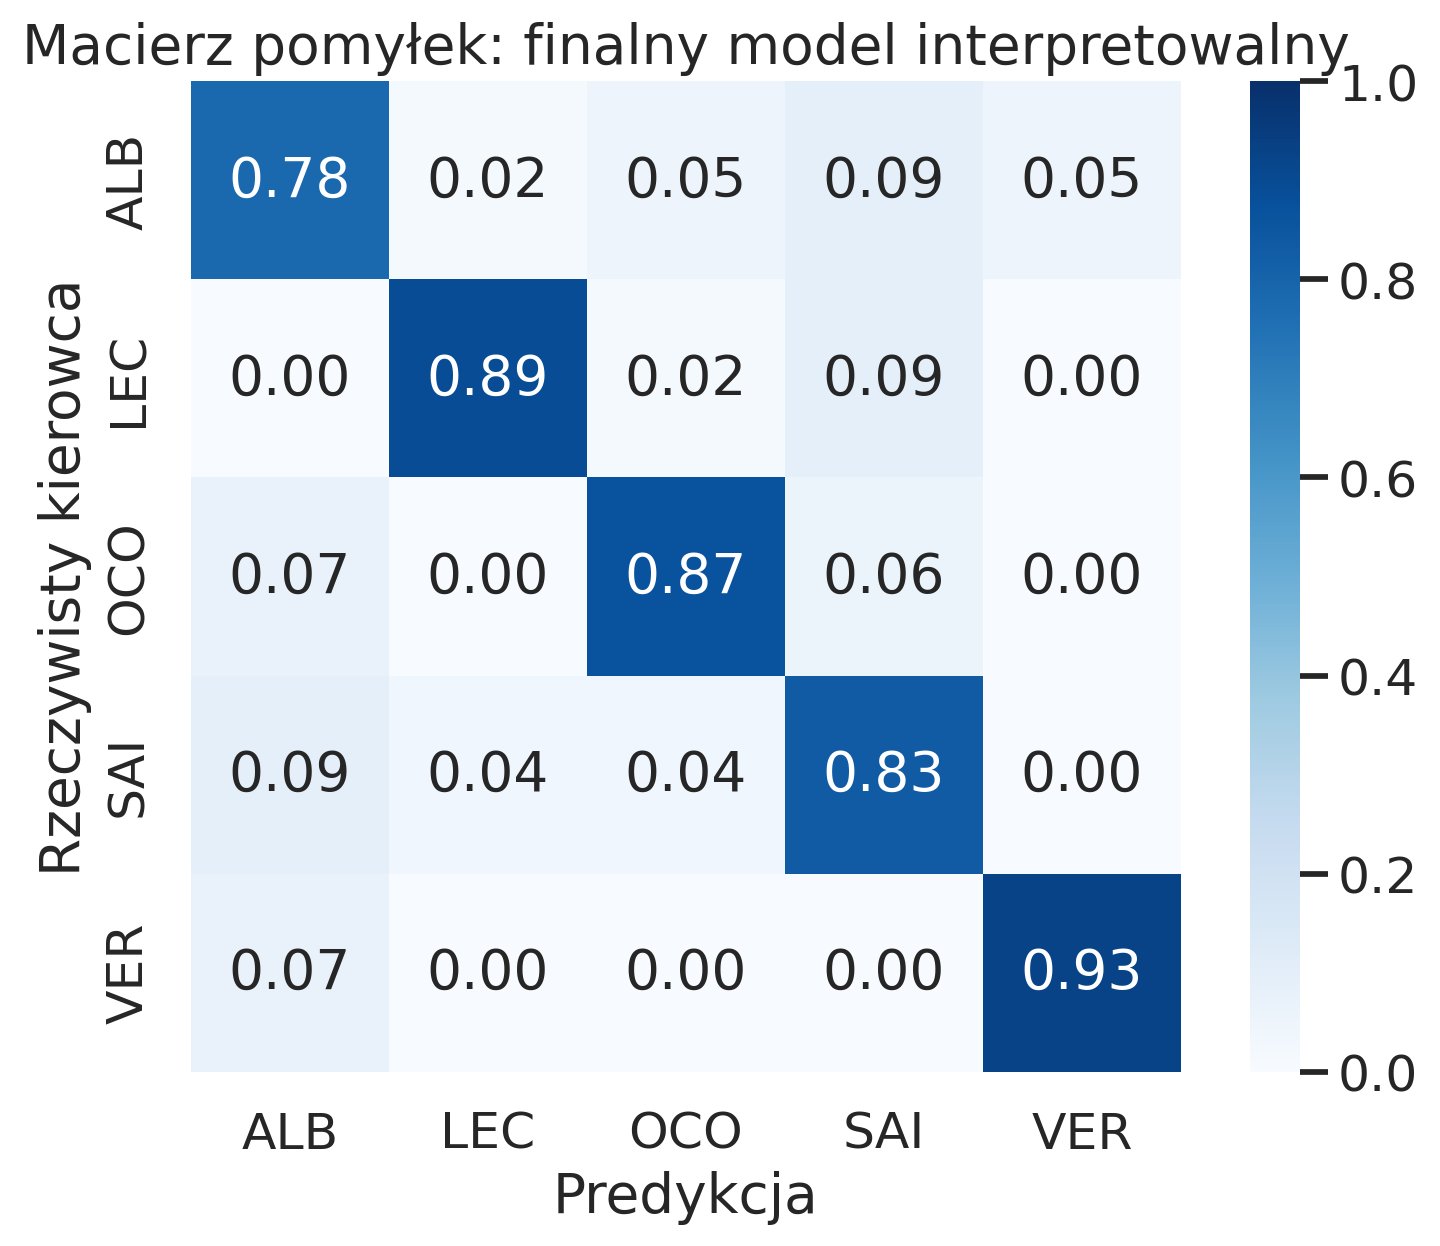
\includegraphics[width=0.70\textwidth]{05_final_model_confusion_matrix.png}
\caption{Macierz pomyłek finalnego modelu regresji logistycznej w krótkim setupie kwalifikacyjnym.}
\label{fig:final-confusion}
\end{figure}

Ten wynik jest zgodny z ogólnym kierunkiem badań nad identyfikacją kierowcy z danych pojazdu, w których zakłada się, że indywidualne zachowania kierowcy są widoczne w sygnałach takich jak prędkość, hamowanie czy przyspieszanie \cite{hallac2016,wang2017}. W danych Formuły 1 problem jest trudniejszy, ponieważ kierowcy jeżdżą dużo bardziej podobnie pod względem celu: wszyscy starają się uzyskać możliwie najlepszy czas. Stabilny wynik w takim środowisku sugeruje, że nawet na bardzo wysokim poziomie sportowym pozostaje mierzalna indywidualna różnica w przebiegu okrążenia.

Istotnym elementem tej części było sprawdzanie, czy wynik nie wynika wyłącznie z prostego tempa okrążenia. Dlatego w kolejnych wariantach usuwano bezpośrednie cechy czasowe, takie jak \texttt{LapTimeSeconds} oraz czasy sektorów. W setupie wyścigowym najlepszy wariant regresji logistycznej bez cech czasowych i bez części kontekstu wyścigowego uzyskał 0.8177 macro F1, czyli wynik praktycznie taki sam jak warianty zawierające więcej informacji kontekstowej. Sugeruje to, że model nie opiera się wyłącznie na tym, kto był szybszy na okrążeniu.

\section{Model sekwencyjny CNN}

Drugim krokiem było przejście od cech zagregowanych do pełnej sekwencji telemetrycznej. W tym podejściu okrążenie było reprezentowane jako przebieg sygnałów \texttt{Speed}, \texttt{Throttle}, \texttt{Brake}, \texttt{RPM} i \texttt{nGear}. Sekwencje były resamplowane do stałej długości, aby mogły być wejściem sieci neuronowej.

Model \texttt{1D CNN} okazał się bardzo mocnym wariantem. W krótkim setupie kwalifikacyjnym poprawił wynik względem regresji logistycznej z 0.8617 do 0.8952 macro F1. W długim setupie kwalifikacyjnym 2018--2025 był najlepszym modelem spośród pierwotnie porównanych architektur i osiągnął 0.9012 macro F1.

\begin{figure}[H]
\centering
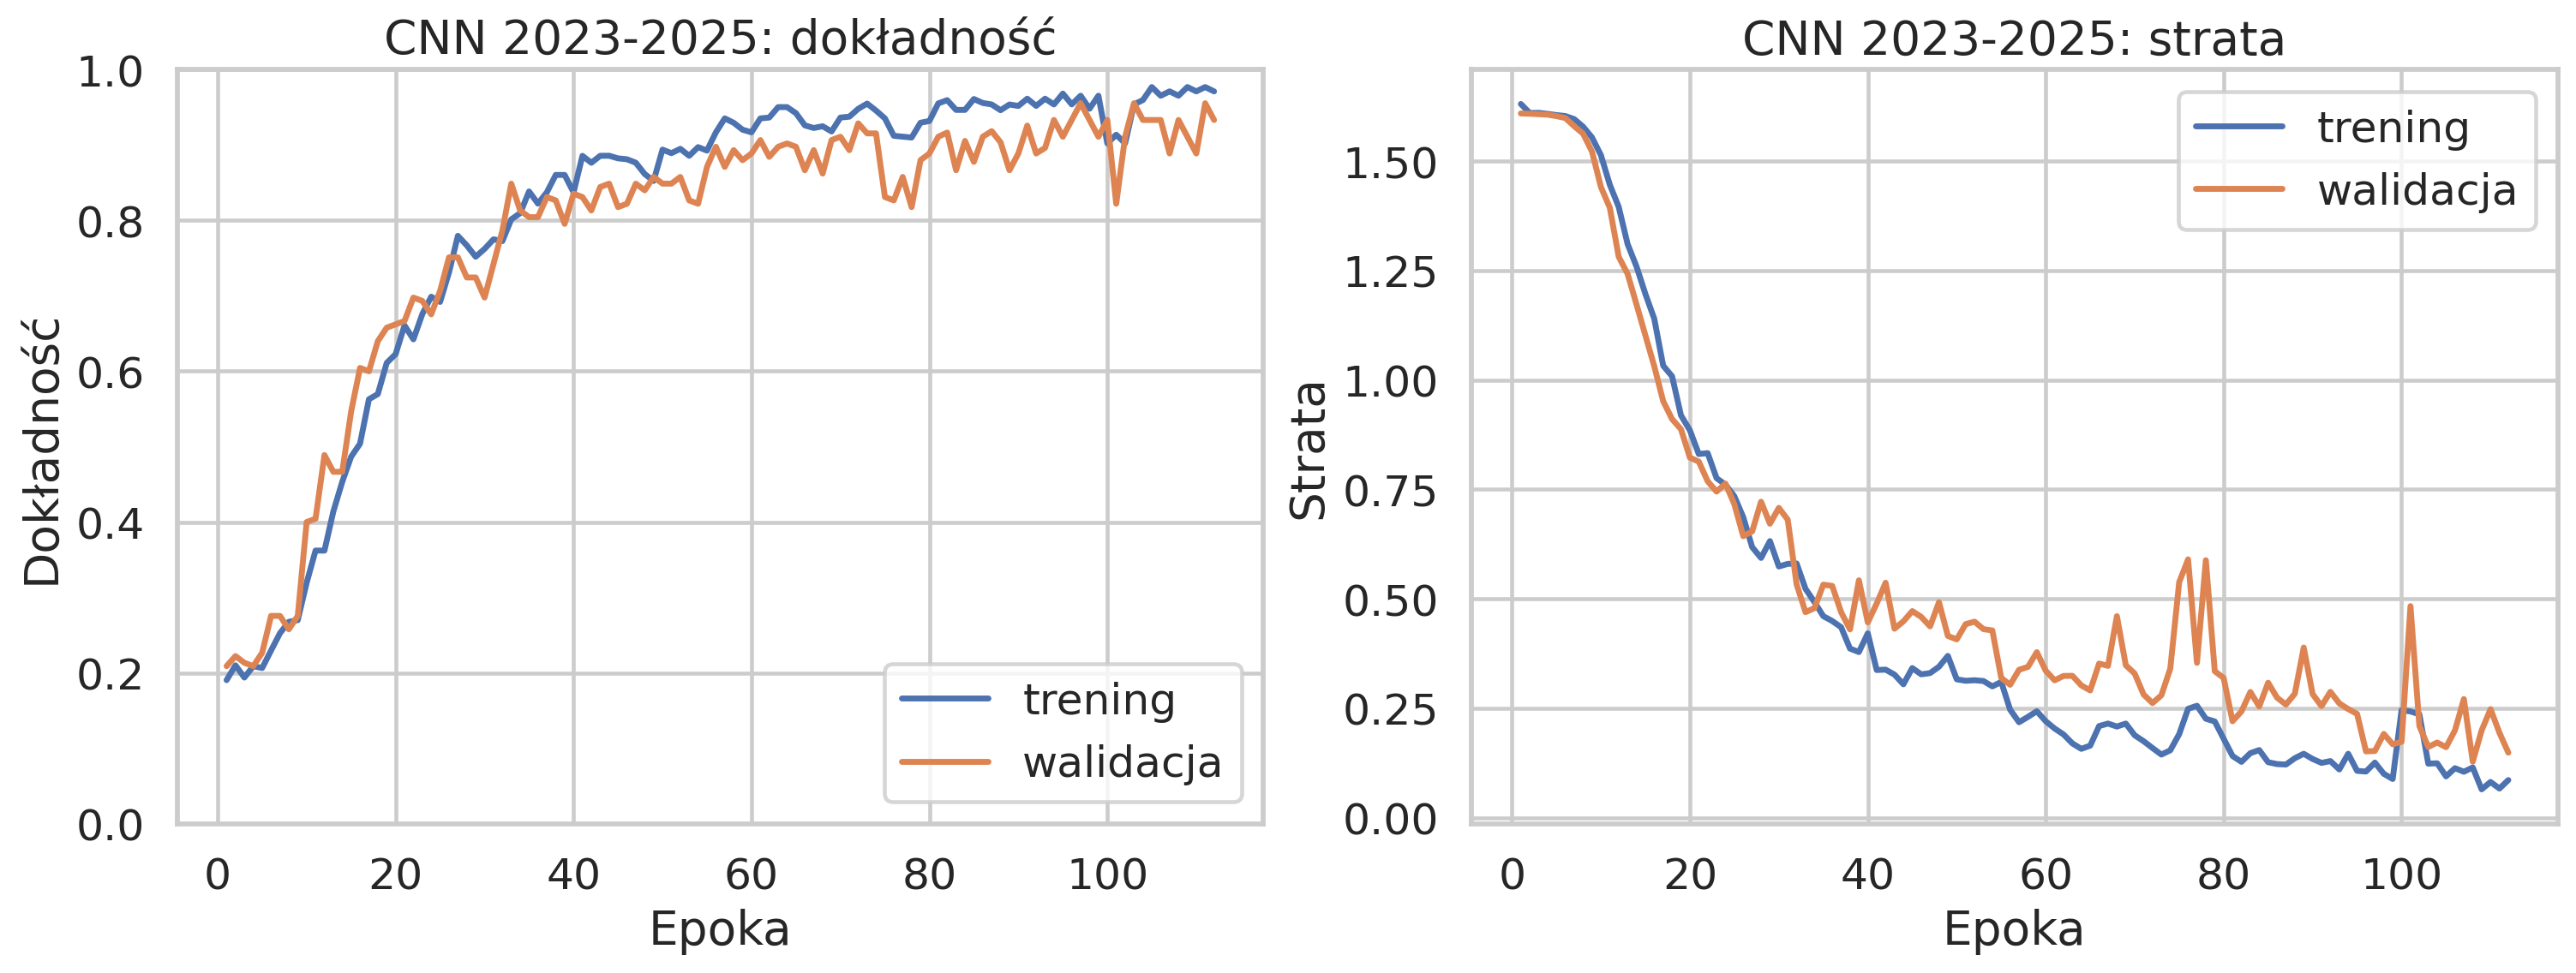
\includegraphics[width=0.90\textwidth]{03_cnn_training_curve_short_horizon.png}
\caption{Przykładowa krzywa uczenia modelu CNN w krótkim setupie kwalifikacyjnym.}
\label{fig:cnn-training-short}
\end{figure}

Lepszy wynik \texttt{CNN} jest spójny z podejściem, w którym zachowanie kierowcy traktuje się jako problem klasyfikacji szeregów czasowych \cite{hallac2016}. W takim ujęciu istotna jest nie tylko średnia wartość cechy, ale także kształt fragmentu sygnału. W przypadku Formuły 1 może to oznaczać sekwencję: odjęcie gazu, hamowanie, redukcje biegów, minimalna prędkość i powrót na gaz. Model konwolucyjny może wychwycić takie lokalne wzorce bez konieczności ręcznego opisywania każdego zakrętu.

\section{Model hybrydowy CNN + cechy tabularne}

Następnie sprawdzono model hybrydowy, który łączył reprezentację sekwencyjną z ręcznie zdefiniowanymi cechami tabularnymi. Przyjęto założenie, że \texttt{CNN} może wychwycić lokalne wzorce przebiegu telemetrii, a cechy tabularne uzupełniają je o syntetyczne informacje o całym okrążeniu.

Ten wariant był najlepszy w krótkim setupie kwalifikacyjnym oraz w setupie wyścigowym. W kwalifikacjach 2023--2025 uzyskał 0.9147 macro F1, a w czystych okrążeniach wyścigowych 2025 uzyskał 0.8564 macro F1.

\begin{figure}[H]
\centering
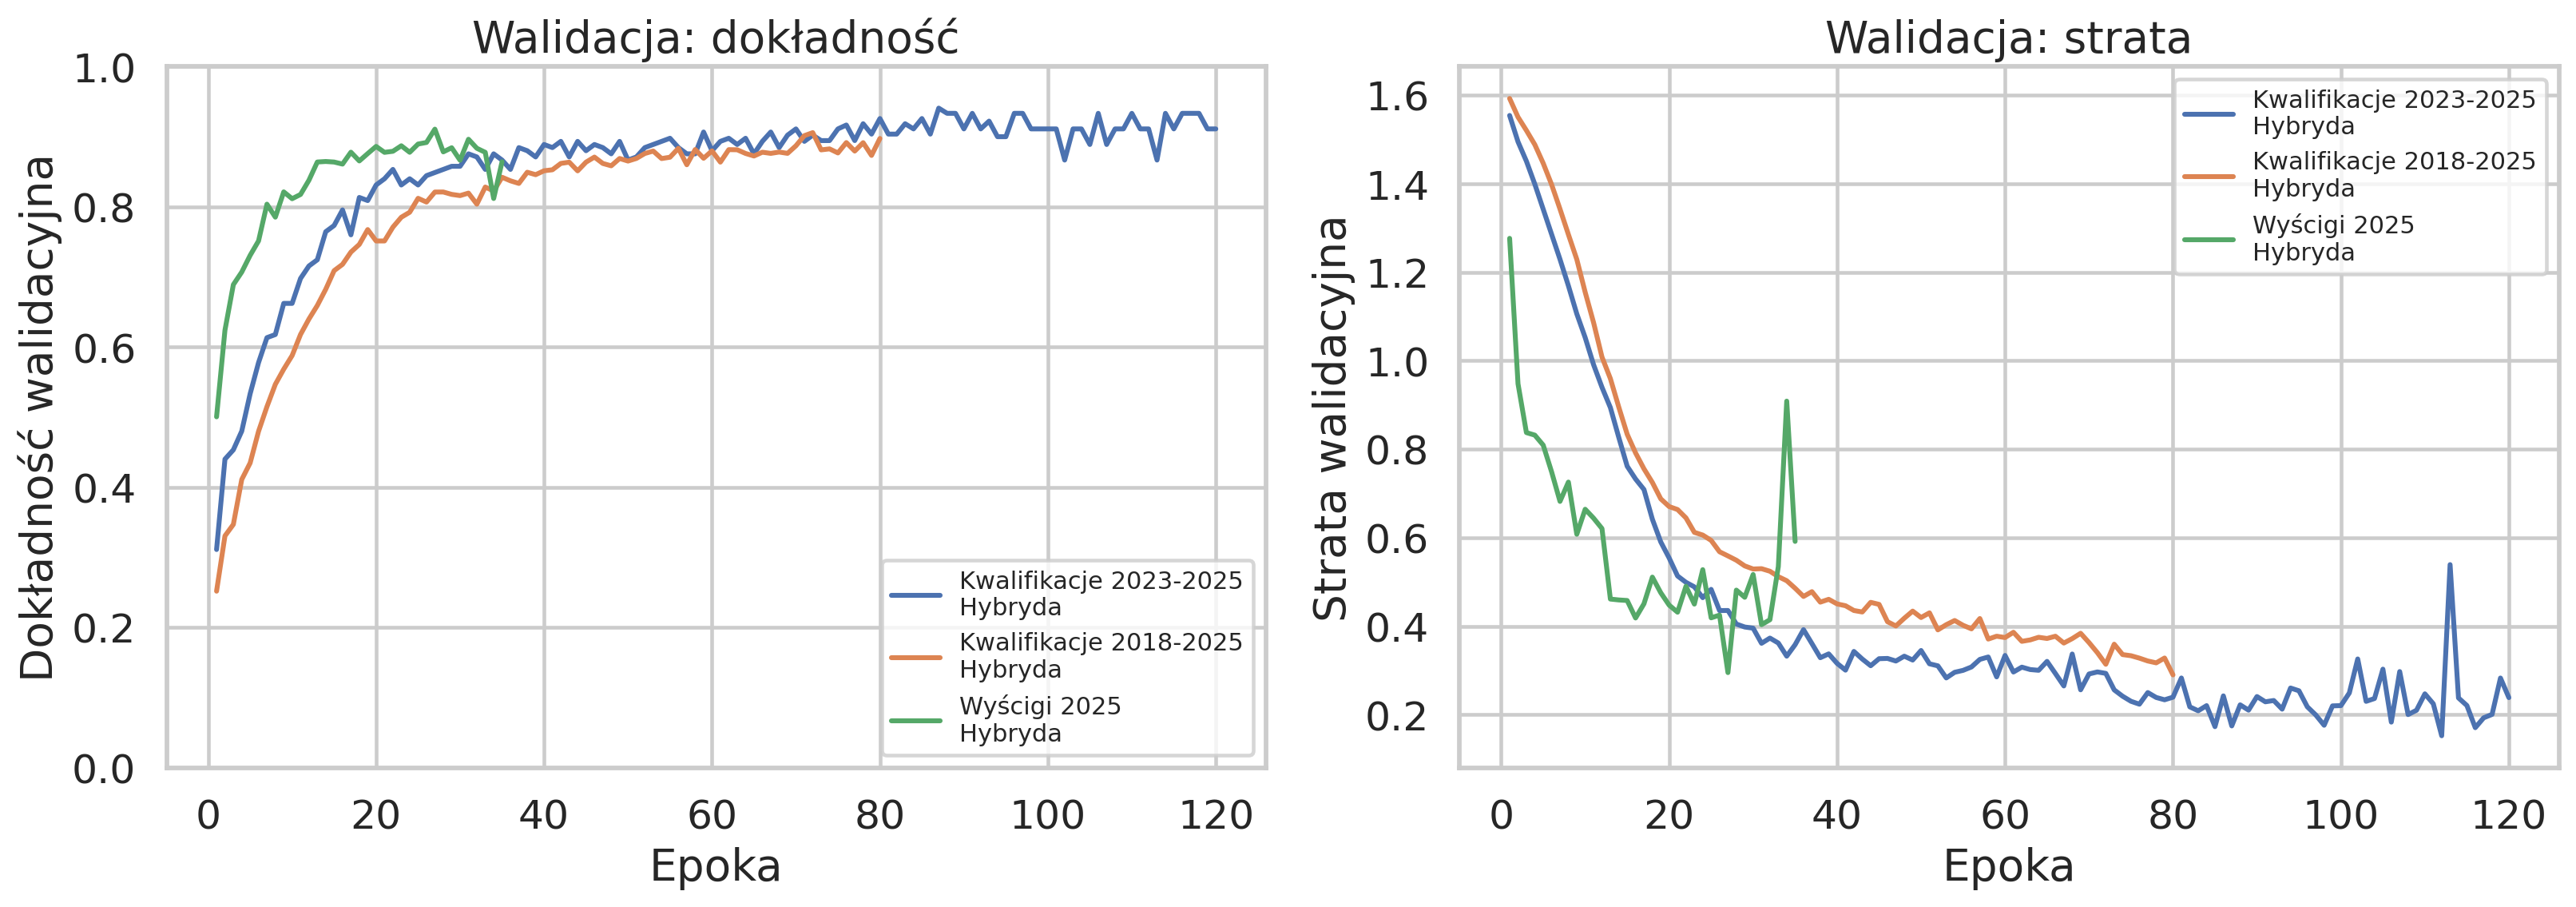
\includegraphics[width=0.95\textwidth]{10_training_curves_multisetup_hybrid.png}
\caption{Krzywe uczenia modelu hybrydowego w trzech setupach.}
\label{fig:training-curves}
\end{figure}

Na wykresie widać, że liczba faktycznie wykonanych epok nie jest identyczna dla każdego setupu. Wynika to z użycia \emph{early stoppingu}. Modele miały ustalony maksymalny limit epok, ale trening był zatrzymywany wcześniej, jeżeli wynik walidacyjny przestawał się poprawiać. Jest to celowe: wymuszanie tej samej liczby epok mogłoby zwiększać przeuczenie i nie byłoby bardziej uczciwym porównaniem. Bardziej porównywalne jest użycie tej samej procedury zatrzymania, tego samego typu walidacji i raportowanie wyniku na foldach testowych. Krótszy trening hybrydy w setupie wyścigowym oznacza więc, że model szybciej doszedł do najlepszego punktu walidacyjnego, a nie że był trenowany mniej starannie.

\begin{figure}[H]
\centering
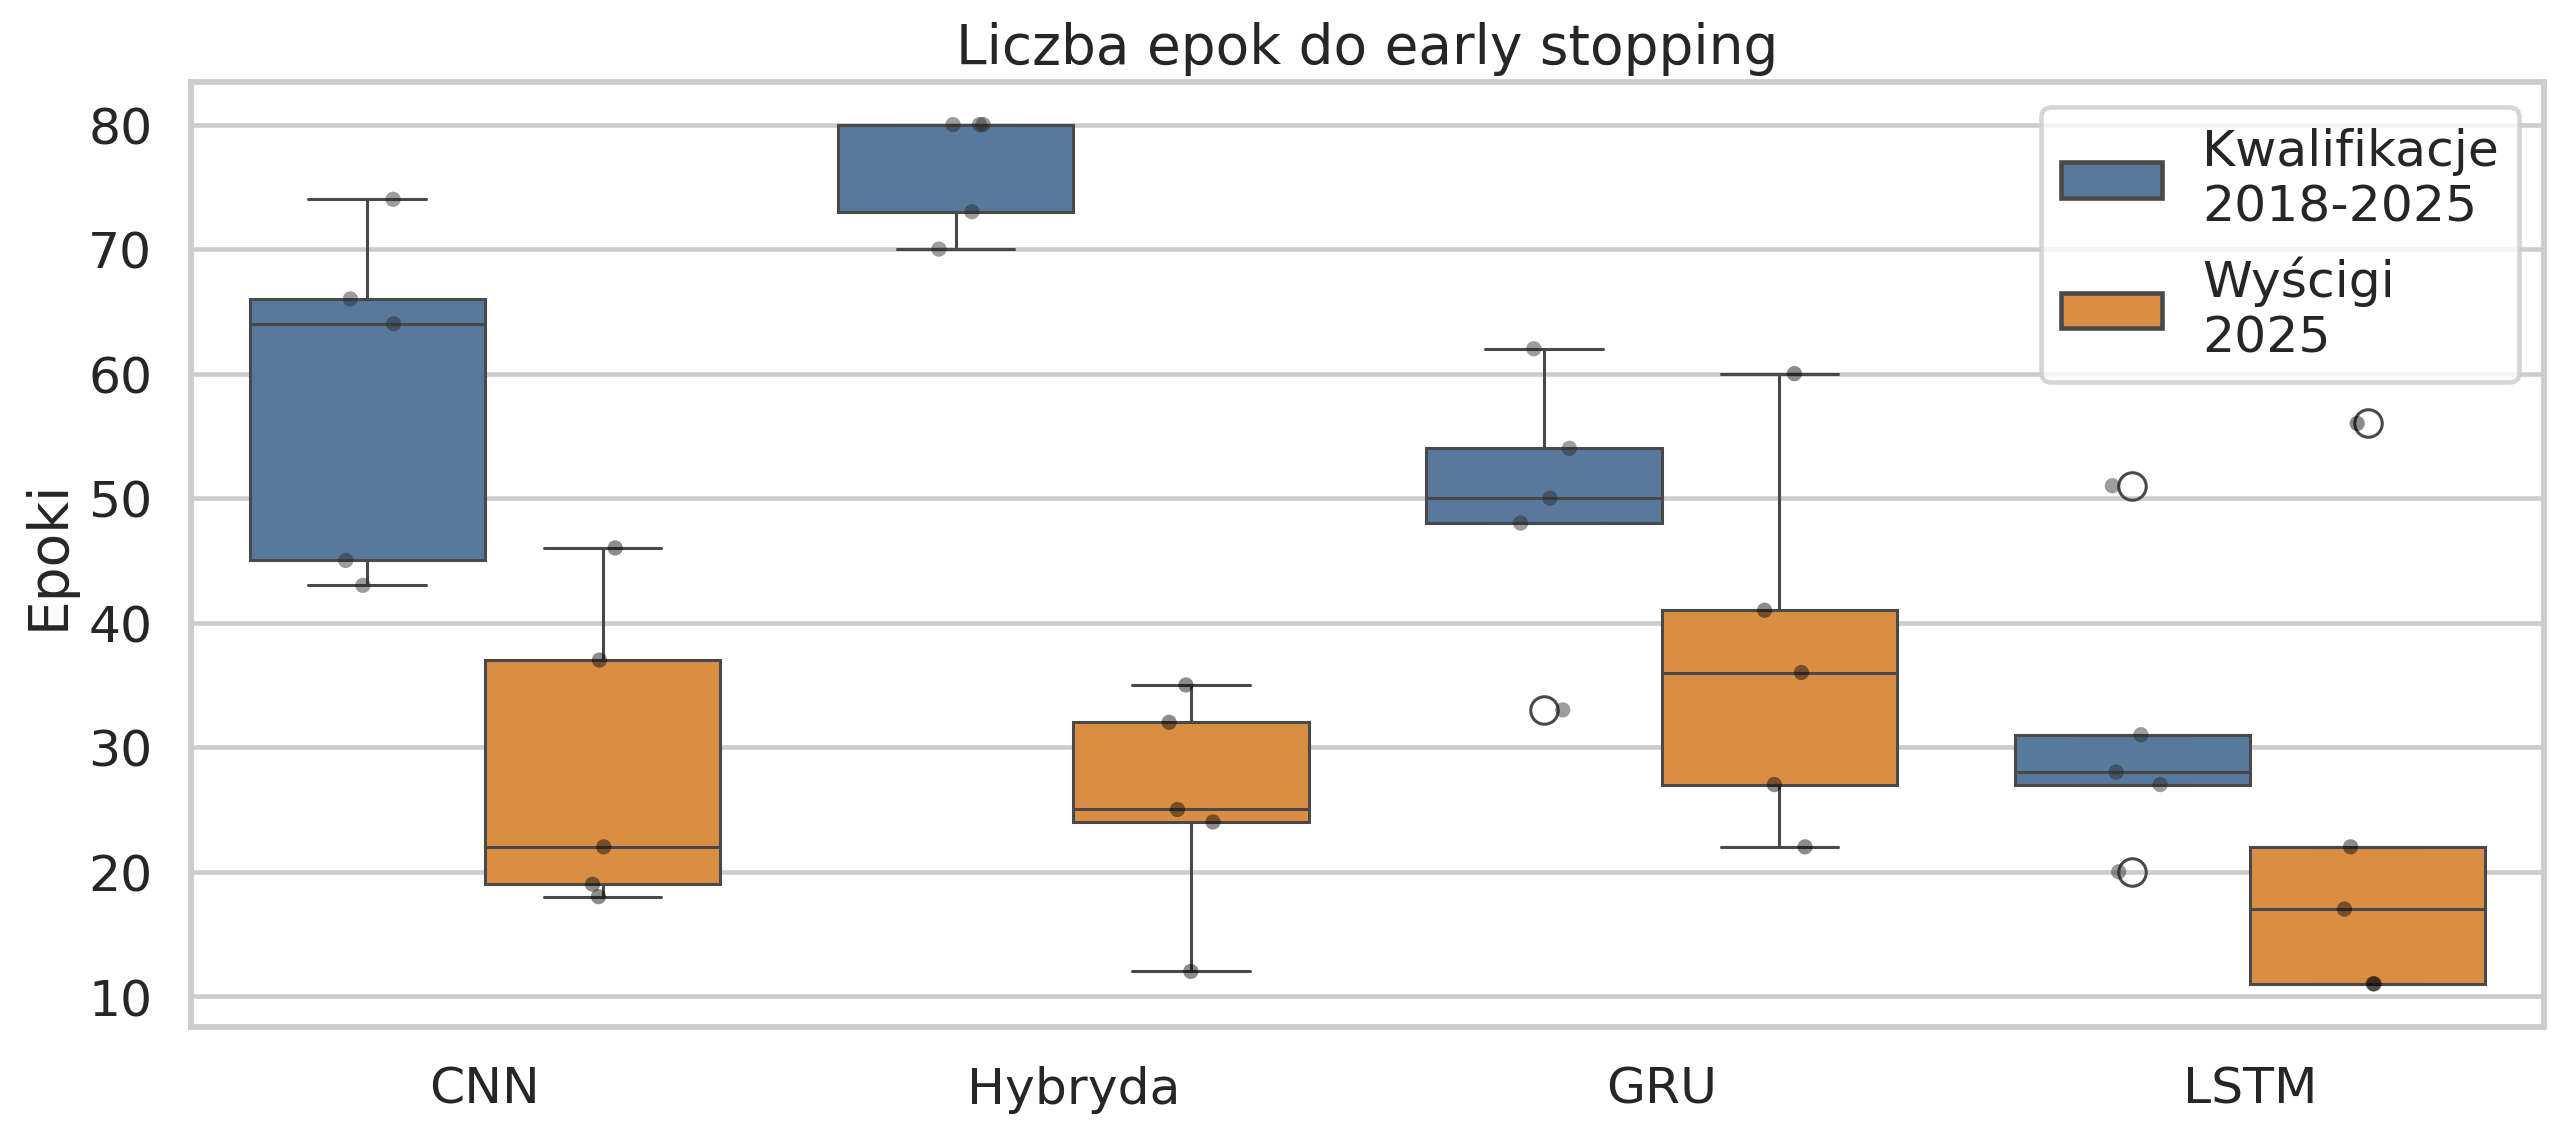
\includegraphics[width=0.85\textwidth]{04_epochs_to_early_stopping.png}
\caption{Liczba epok wykonanych przed zatrzymaniem treningu w modelach sekwencyjnych.}
\label{fig:epochs-early-stopping}
\end{figure}
\FloatBarrier

\section{GRU i LSTM}

Dla porównania sprawdzono również architektury rekurencyjne \texttt{GRU} i \texttt{LSTM}. Ich wyniki były wyraźnie słabsze od \texttt{CNN} i hybrydy. W krótkim setupie kwalifikacyjnym \texttt{GRU} uzyskał 0.4595 macro F1, a \texttt{LSTM} 0.3365. W długim setupie kwalifikacyjnym oraz w setupie wyścigowym ich wyniki poprawiały się tylko częściowo i nie zmieniły ogólnego rankingu architektur.

Jedna z możliwych interpretacji jest taka, że w tych danych najważniejsze są lokalne wzorce i kształt fragmentów telemetrii, które \texttt{CNN} rozpoznaje efektywniej niż modele rekurencyjne. Nie oznacza to, że \texttt{GRU} i \texttt{LSTM} są ogólnie słabymi architekturami, tylko że w tej konkretnej reprezentacji danych nie były najlepszym wyborem.

\section{Zestawienie końcowe modeli}

Tabela~\ref{tab:model-results} przedstawia najważniejsze wyniki dla trzech setupów.

\begin{table}[H]
\centering
\small
\begin{tabular}{lccccc}
\toprule
Setup & Regresja logistyczna & CNN & Hybryda & GRU & LSTM \\
\midrule
Kwalifikacje 2023--2025 & 0.8617 & 0.8952 & \textbf{0.9147} & 0.4595 & 0.3365 \\
Kwalifikacje 2018--2025 & 0.8267 & \textbf{0.9012} & 0.8887 & 0.2880 & 0.2998 \\
Wyścigi 2025 & 0.8177 & 0.8466 & \textbf{0.8564} & 0.5639 & 0.3216 \\
\bottomrule
\end{tabular}
\caption{Macro F1 dla głównych rodzin modeli.}
\label{tab:model-results}
\end{table}

\begin{figure}[H]
\centering
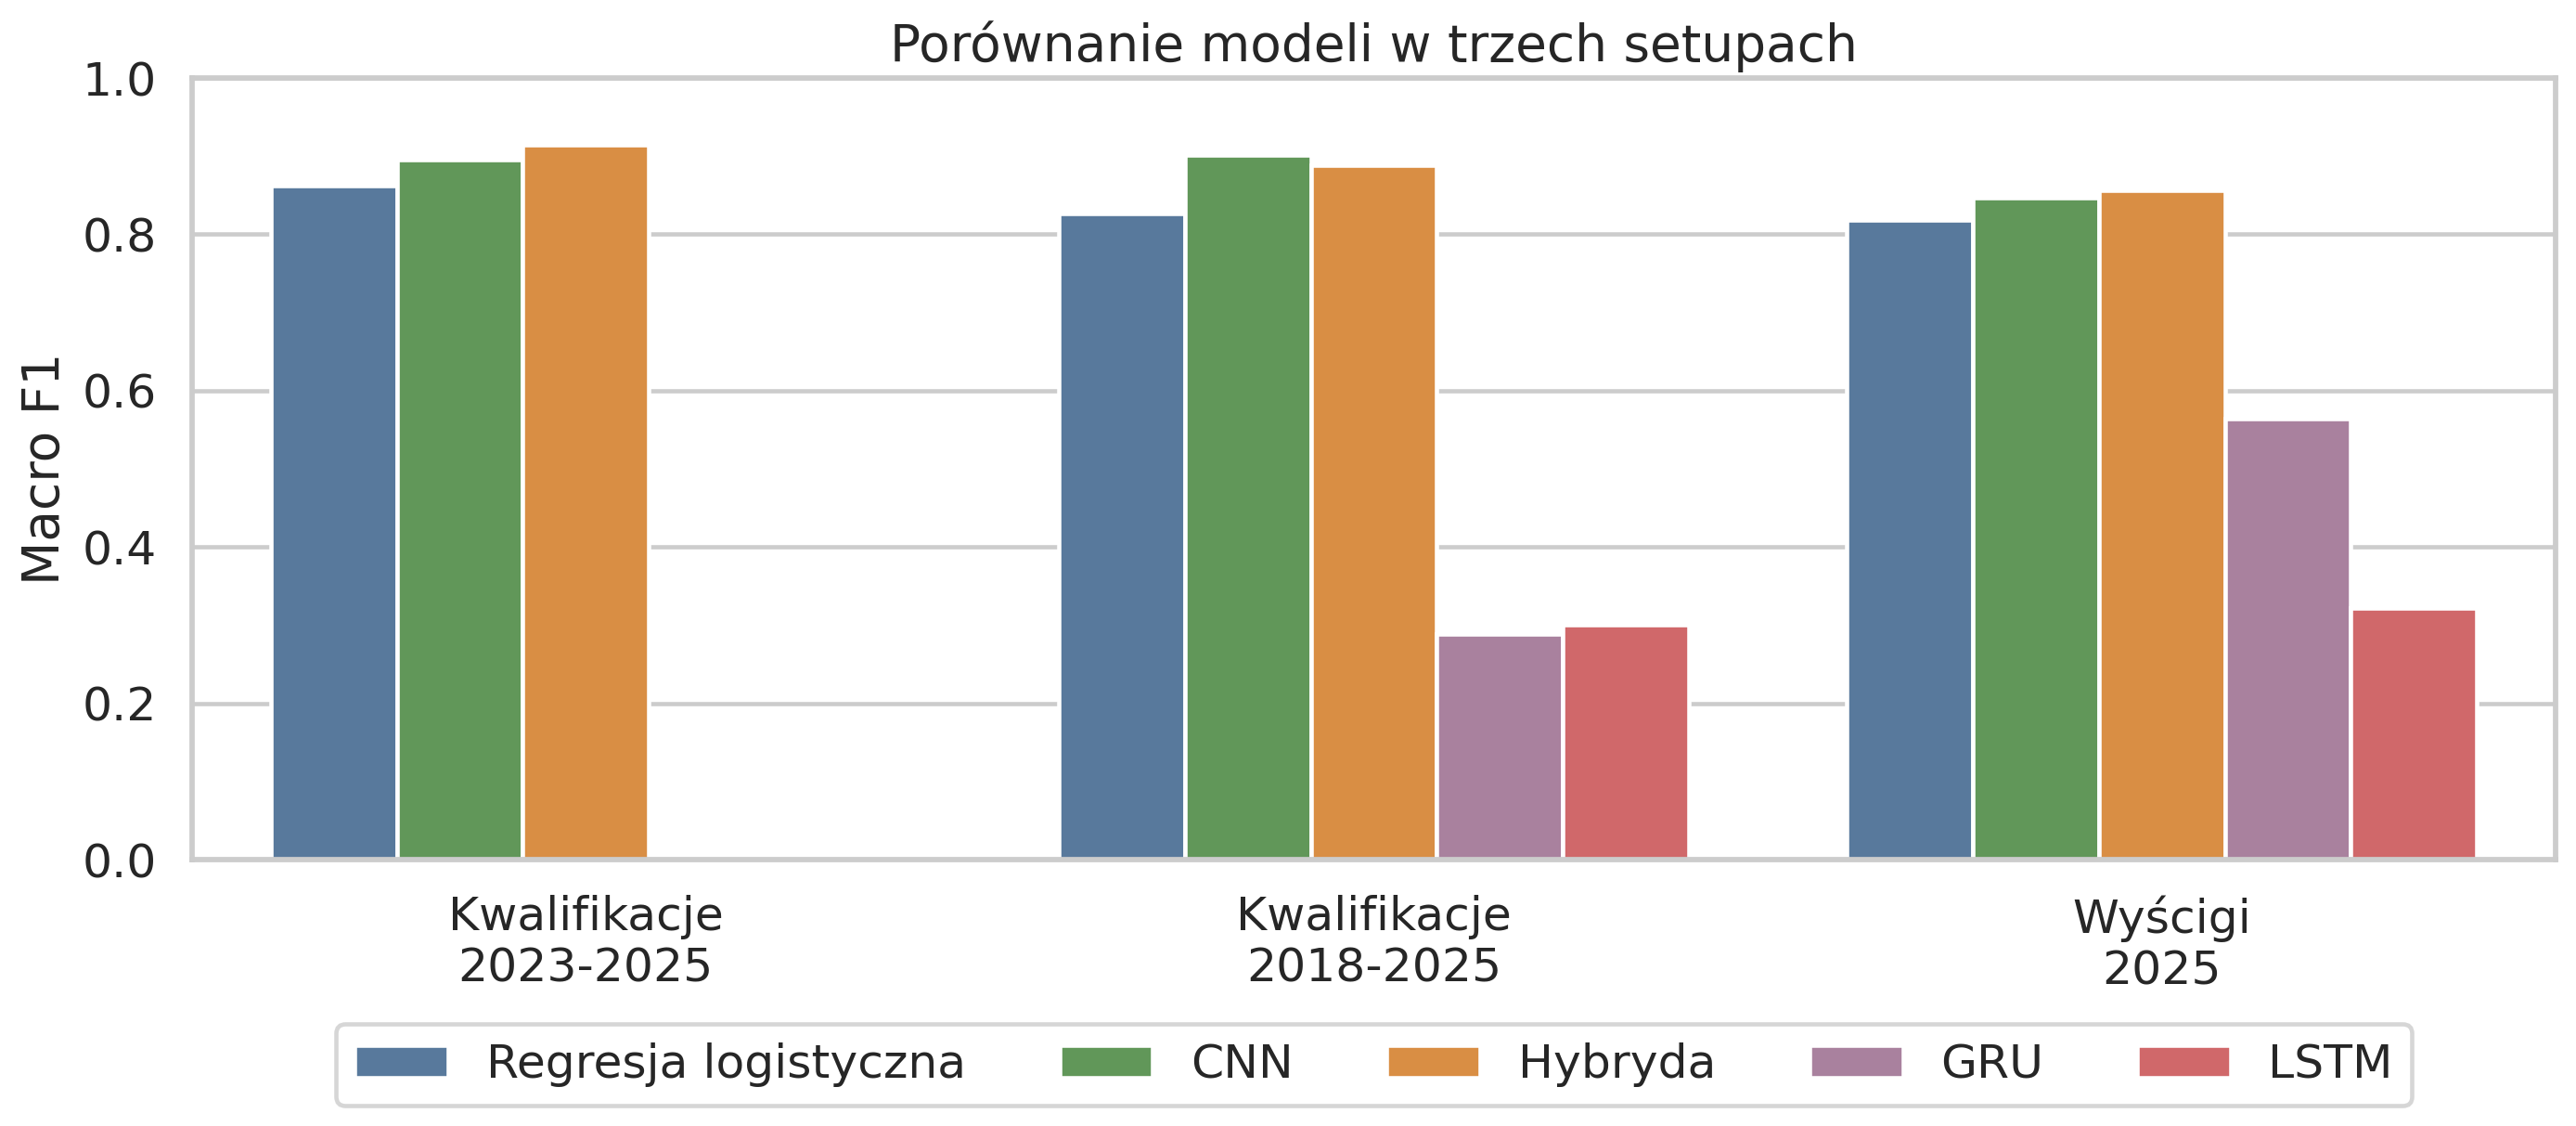
\includegraphics[width=0.95\textwidth]{02_model_progression.png}
\caption{Porównanie wyników modeli w trzech setupach.}
\label{fig:model-progression}
\end{figure}

Identyfikacja kierowcy na podstawie telemetrii okazała się możliwa we wszystkich trzech setupach. Najwyższe wyniki osiągały modele sekwencyjne i hybrydowe, co sugeruje, że pełny przebieg okrążenia zawiera dodatkową informację względem samych cech zagregowanych.

Wynik ten można zestawić z projektem WithSeismic, w którym opisano identyfikację kierowców F1 na podstawie dużej liczby fragmentów zakrętów \cite{withseismic2026}. Uzyskany tam wynik był istotnie lepszy od losowego, ale niższy niż w prezentowanej analizie. Nie jest to bezpośrednio porównywalny eksperyment, ponieważ tam analizowano fragmenty zakrętów z innego źródła danych i z innym podziałem problemu, natomiast tutaj klasyfikowane są pełne okrążenia w wybranych setupach. Sam kierunek jest jednak podobny: telemetria zawiera mierzalny ślad kierowcy, ale jakość wyniku zależy od definicji próbki, liczby klas i sposobu walidacji.

\begin{figure}[H]
\centering
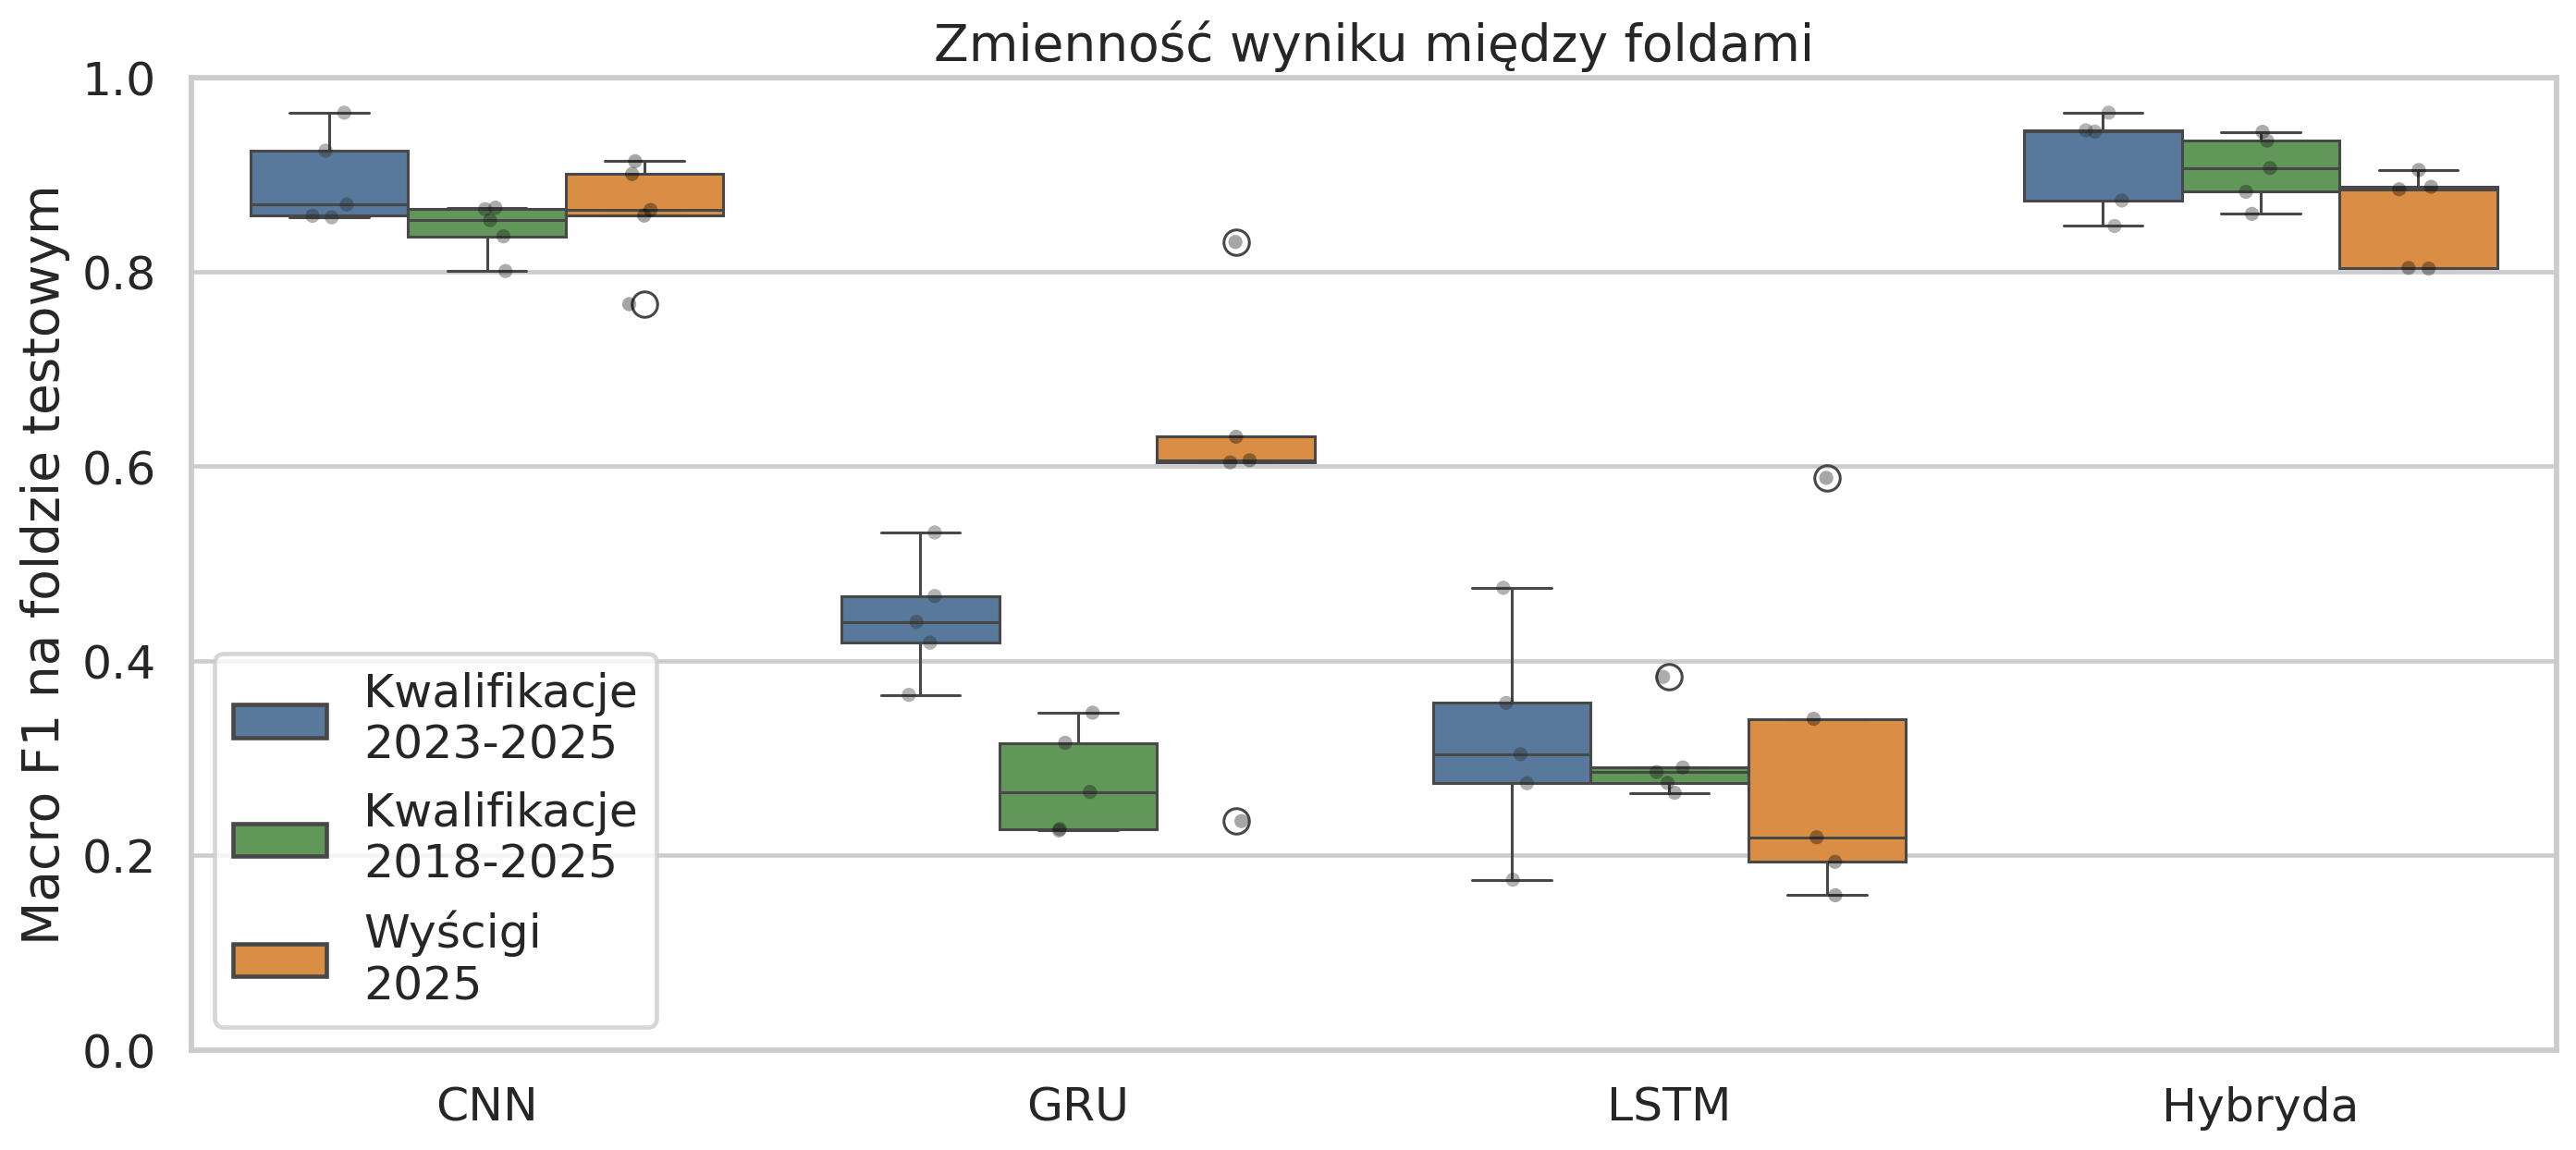
\includegraphics[width=0.95\textwidth]{11_sequence_fold_variability.png}
\caption{Zmienność wyniku między foldami walidacji.}
\label{fig:fold-variability}
\end{figure}

Wyniki między foldami pokazują, że jakość modelu zależy od konkretnego podziału sesji, ale ogólny ranking architektur pozostaje spójny. Najlepiej wypadają modele \texttt{CNN} i hybrydowe, natomiast \texttt{GRU} i \texttt{LSTM} są słabsze.

\section{Macierze pomyłek}

Macierze pomyłek najlepszych modeli pokazano na rysunku~\ref{fig:sequence-confusion}.

\begin{figure}[H]
\centering
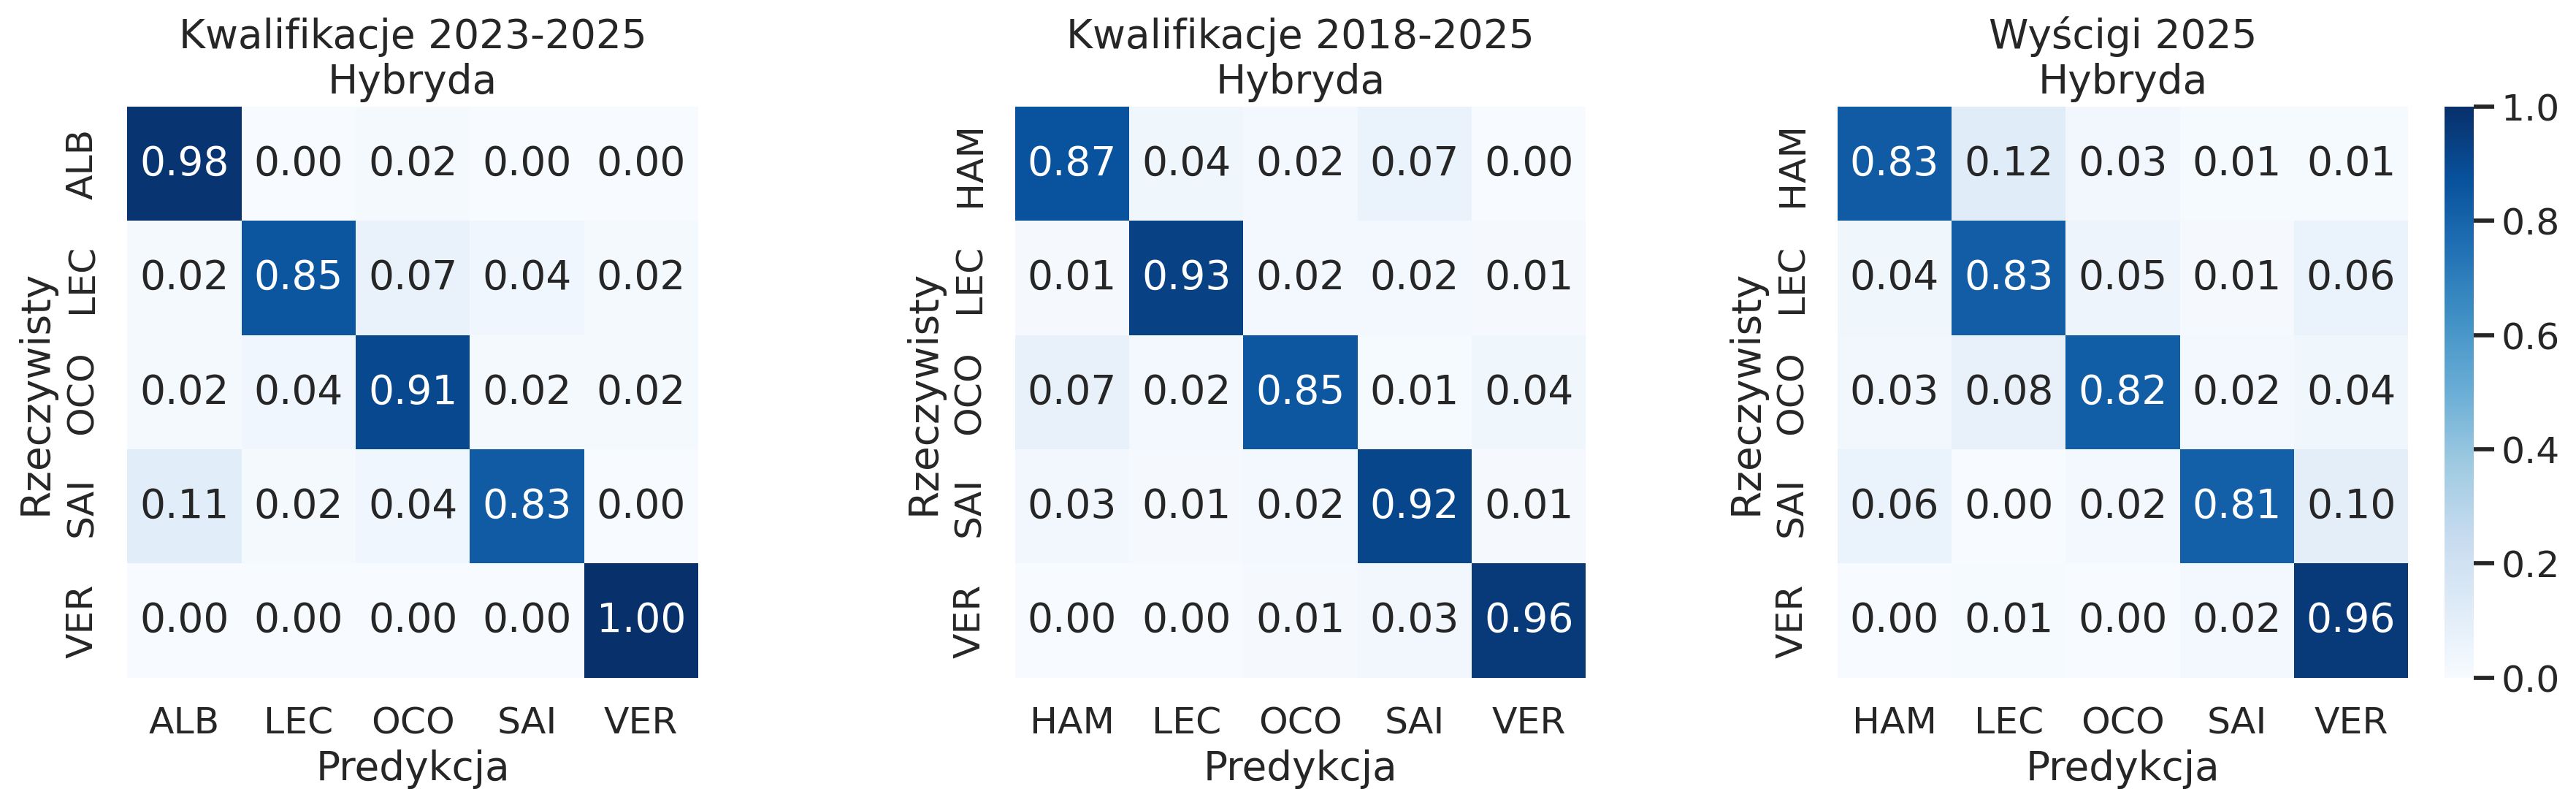
\includegraphics[width=0.95\textwidth]{12_best_sequence_confusion_matrices.png}
\caption{Macierze pomyłek najlepszych modeli sekwencyjnych i hybrydowych.}
\label{fig:sequence-confusion}
\end{figure}
\FloatBarrier

Macierze pomyłek pozwalają sprawdzić, którzy kierowcy są rozpoznawani najlepiej, a które pary są mylone. Wysoki wynik globalny nie wystarcza do zrozumienia, czy model faktycznie rozpoznaje każdego kierowcę.

\section{Interpretacja cech}

Najważniejsze cechy modelu pokazano na rysunku~\ref{fig:feature-importance}.

\begin{figure}[H]
\centering
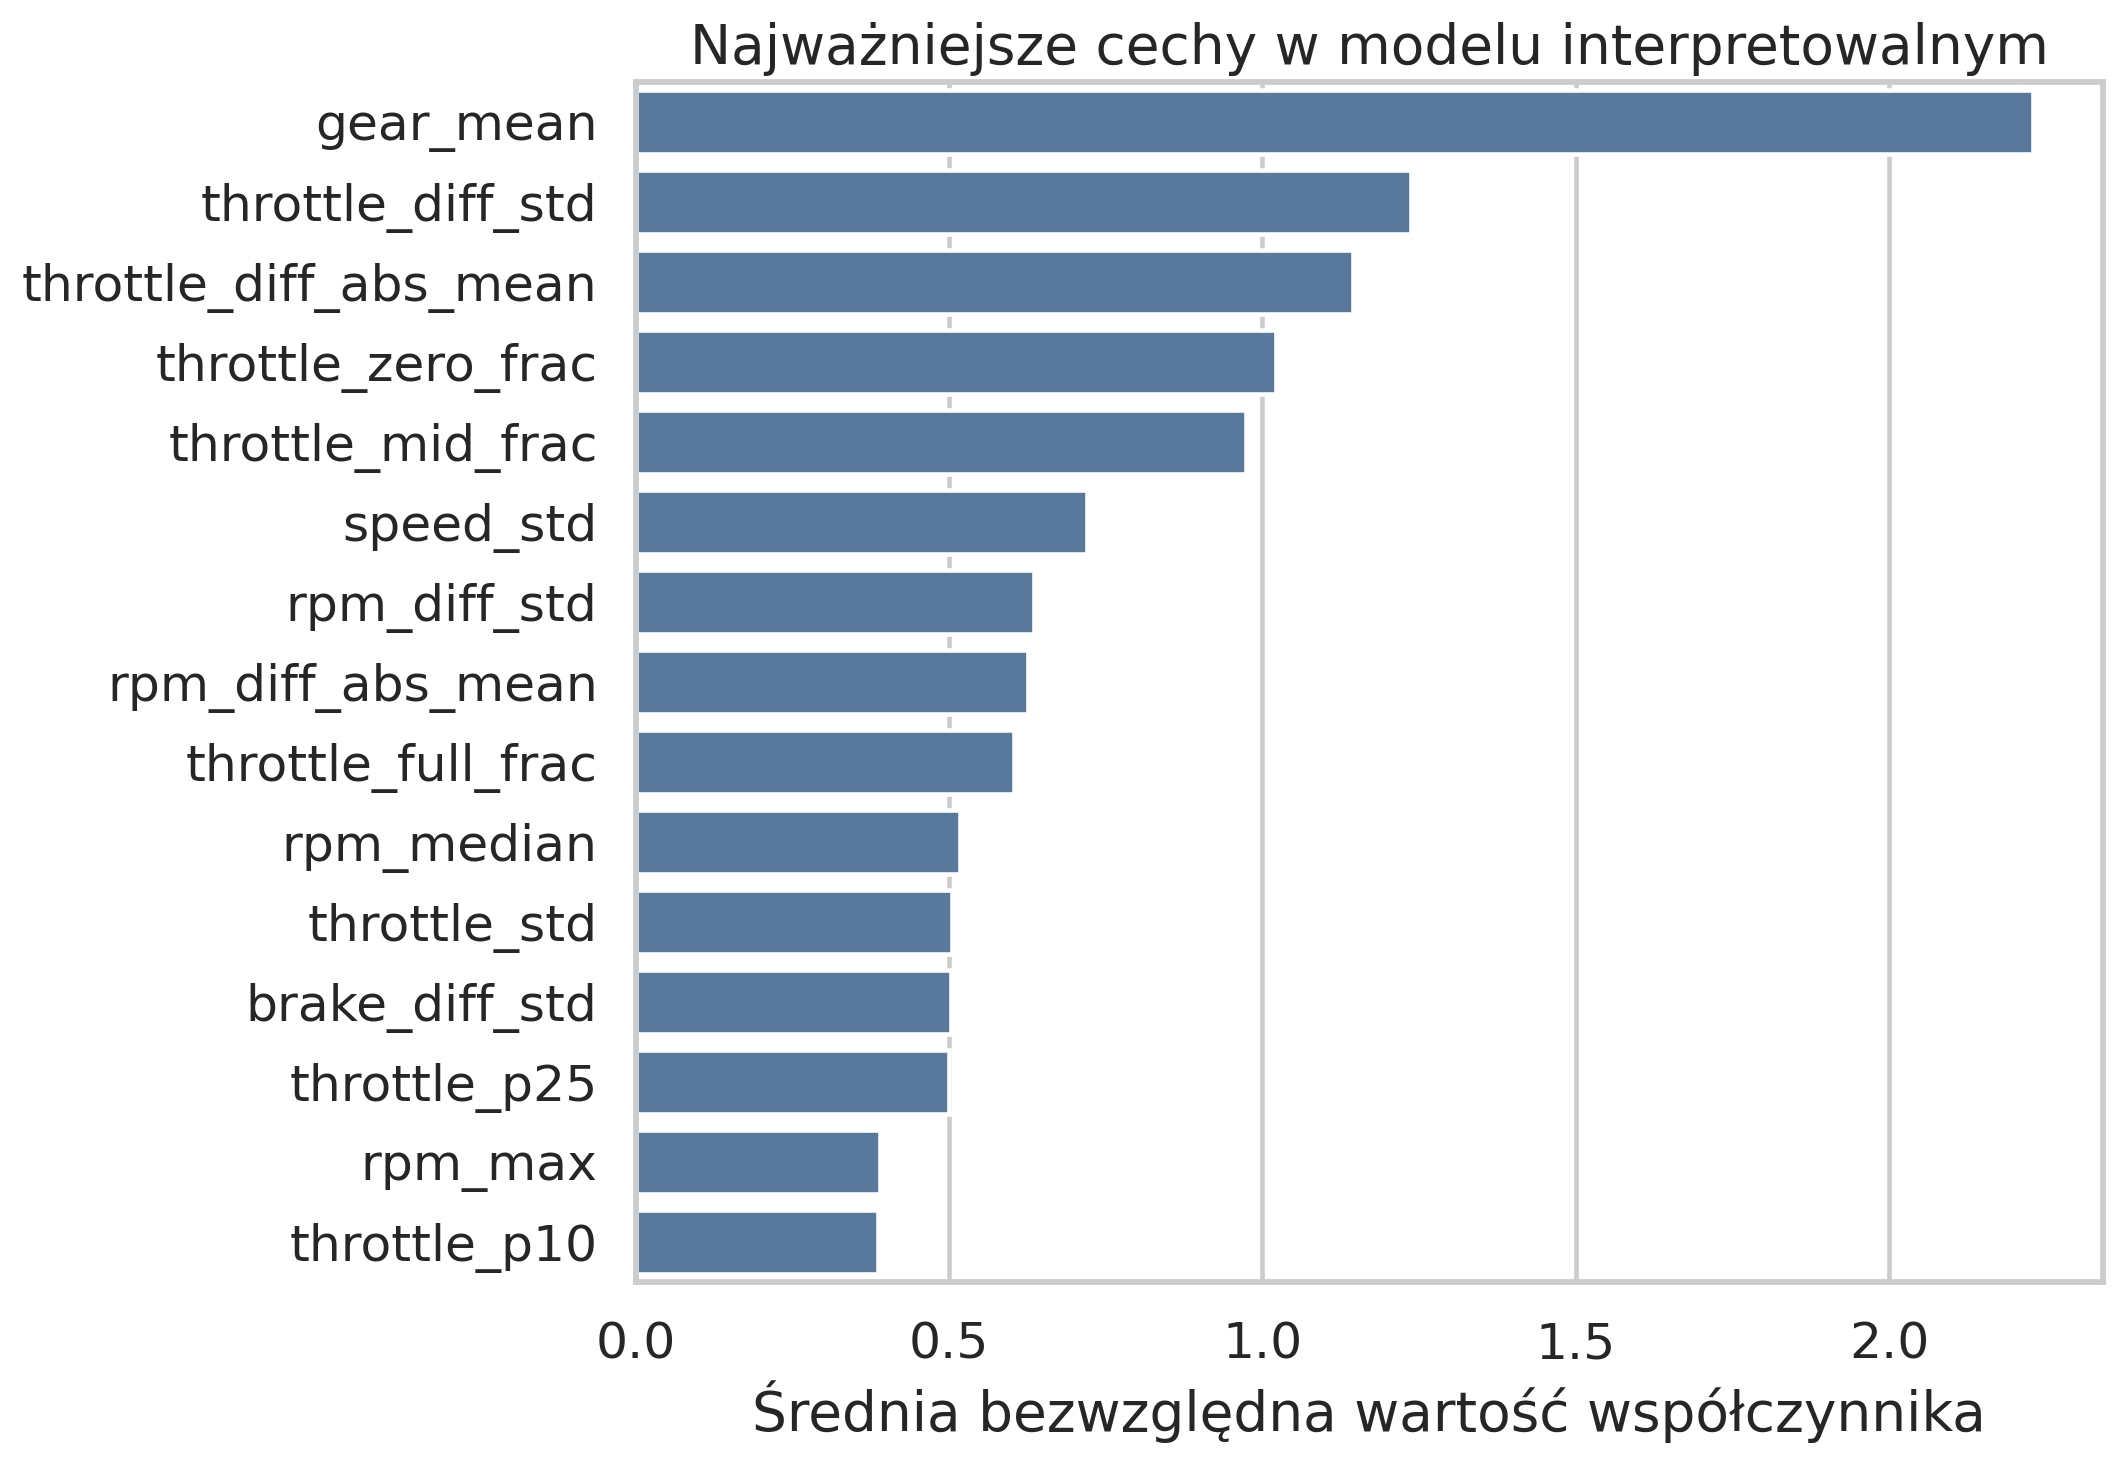
\includegraphics[width=0.85\textwidth]{06_driver_feature_importance.png}
\caption{Najważniejsze cechy w modelu interpretowalnym.}
\label{fig:feature-importance}
\end{figure}

Najważniejsze cechy modelu interpretowalnego dotyczą przede wszystkim operowania gazem, biegami, obrotami silnika, hamowaniem oraz dynamiką sygnałów. Wskazuje to, że model nie opiera się wyłącznie na prostym tempie okrążenia.

Najwyżej ocenioną cechą w finalnym modelu regresji logistycznej była \texttt{gear\_mean}, czyli średni bieg używany w okrążeniu. Nie należy interpretować tego jako prostego stwierdzenia, że dany kierowca „lubi wyższy bieg”. Ta cecha jest raczej pośrednim opisem profilu okrążenia: prędkości w zakrętach, momentów redukcji, długości faz przyspieszania i tego, jak często kierowca utrzymuje samochód w wyższym lub niższym zakresie przełożeń. Wspólnie z cechami przepustnicy i obrotów silnika opisuje rytm prowadzenia samochodu.

Takie znaczenie cech jest zgodne z przeglądami rozpoznawania stylu jazdy, w których zachowanie kierowcy opisuje się między innymi przez przyspieszanie, hamowanie, prędkość i dynamikę manewrów \cite{driving_style_review}. \texttt{gear\_mean} trzeba jednak interpretować ostrożnie, ponieważ może zawierać także informację o samochodzie, torze i sezonie. Nie jest to więc czysta przyczyna stylu jazdy, lecz użyteczny wskaźnik różnic w profilu telemetrycznym. Właśnie dlatego w kolejnym badaniu przeprowadzono osobną analizę biasu zespołowego.

\chapter{Badanie 2: Bias zespołowy i wpływ samochodu}

\section{Motywacja}

Wynik klasyfikacji kierowcy może być zawyżony, jeżeli model uczy się nie tylko stylu kierowcy, ale także charakterystyki samochodu lub zespołu. Dlatego w drugim badaniu sprawdzono, czy z tych samych danych można przewidywać zespół oraz czy predykcja zespołu pomaga w predykcji kierowcy.

\section{Predykcja kierowcy a predykcja zespołu}

Porównanie wyników predykcji kierowcy i zespołu przedstawiono na rysunku~\ref{fig:driver-vs-team}.

\begin{figure}[H]
\centering
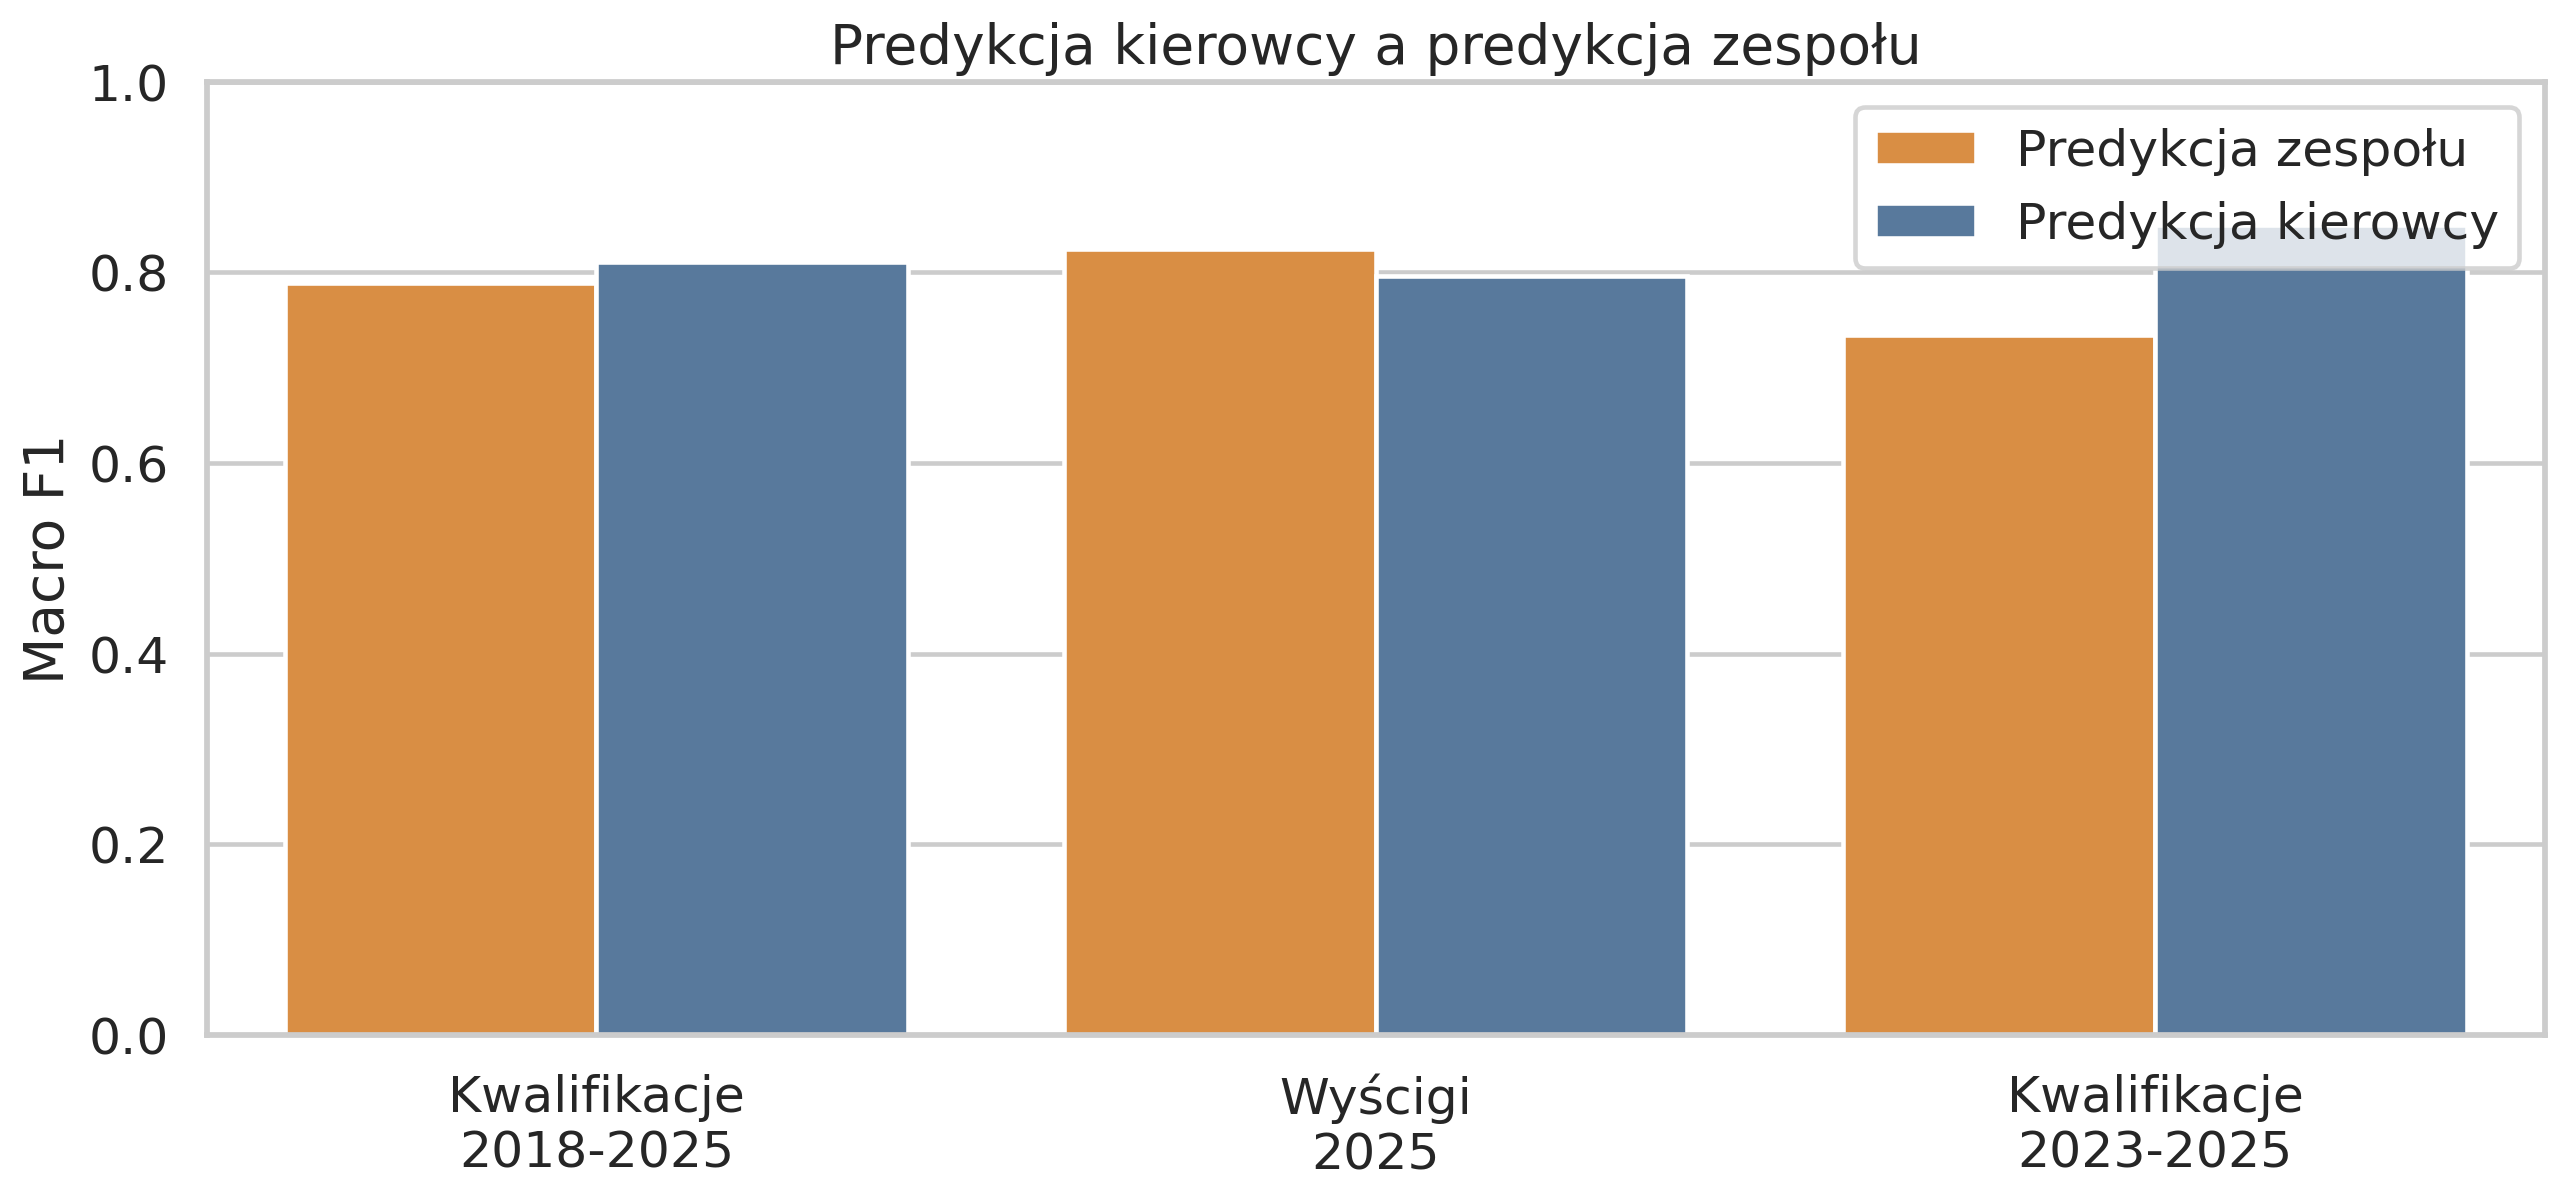
\includegraphics[width=0.90\textwidth]{07_driver_vs_team_prediction.png}
\caption{Porównanie predykcji kierowcy i predykcji zespołu.}
\label{fig:driver-vs-team}
\end{figure}

Zespół również ma wyraźny podpis telemetryczny. Oznacza to obecność realnego biasu zespołowego, którego nie można ignorować przy interpretacji modeli kierowcy. Predykcję zespołu sprawdzono także w wariantach bez bezpośrednich cech czasowych, aby nie sprowadzić zadania wyłącznie do rozpoznawania najszybszych i najwolniejszych samochodów.

\begin{table}[H]
\centering
\small
\begin{tabular}{lccc}
\toprule
Setup & Liczba klas zespołów & Konfiguracja cech & Macro F1 \\
\midrule
Kwalifikacje 2023--2025 & 8 & bez czasu i kontekstu & 0.7340 \\
Kwalifikacje 2018--2025 & 6 & bez czasu i kontekstu & 0.7884 \\
Wyścigi 2025 & 4 & wszystkie cechy telemetryczne & 0.8242 \\
\bottomrule
\end{tabular}
\caption{Najlepsze wyniki predykcji zespołu w analizie biasu zespołowego.}
\label{tab:team-prediction}
\end{table}

Intuicyjnie można oczekiwać, że zespół łatwo rozpoznać po czasie okrążenia lub prędkości maksymalnej. Wyniki są ciekawsze, ponieważ dobre rezultaty pojawiały się także po usunięciu cech czasowych. Oznacza to, że model wykrywał nie tylko ogólne tempo, ale również szerszy profil telemetryczny samochodu: sposób osiągania prędkości, zakres pracy biegów, charakterystykę gazu i obrotów.

Ten element odróżnia analizę Formuły 1 od wielu klasycznych prac o identyfikacji kierowcy. W zwykłych danych drogowych zwykle zakłada się, że samochód jest albo stały, albo mniej istotny niż kierowca. W F1 samochód i zespół są częścią problemu: kierowcy prowadzą różne konstrukcje, a charakterystyka auta może wpływać na prędkość, dobór biegów i sposób oddawania mocy. Dlatego wysoki wynik identyfikacji kierowcy wymaga kontroli, czy model nie rozpoznaje w praktyce głównie samochodu.

\section{Model hierarchiczny i team-aware}

Sprawdzono dwa warianty wykorzystania informacji o zespole:

\begin{itemize}
    \item model hierarchiczny, w którym najpierw przewidywany jest zespół, a następnie kierowca;
    \item model team-aware, w którym prawdopodobieństwa zespołu są dodatkowymi cechami dla modelu kierowcy.
\end{itemize}

\begin{figure}[H]
\centering
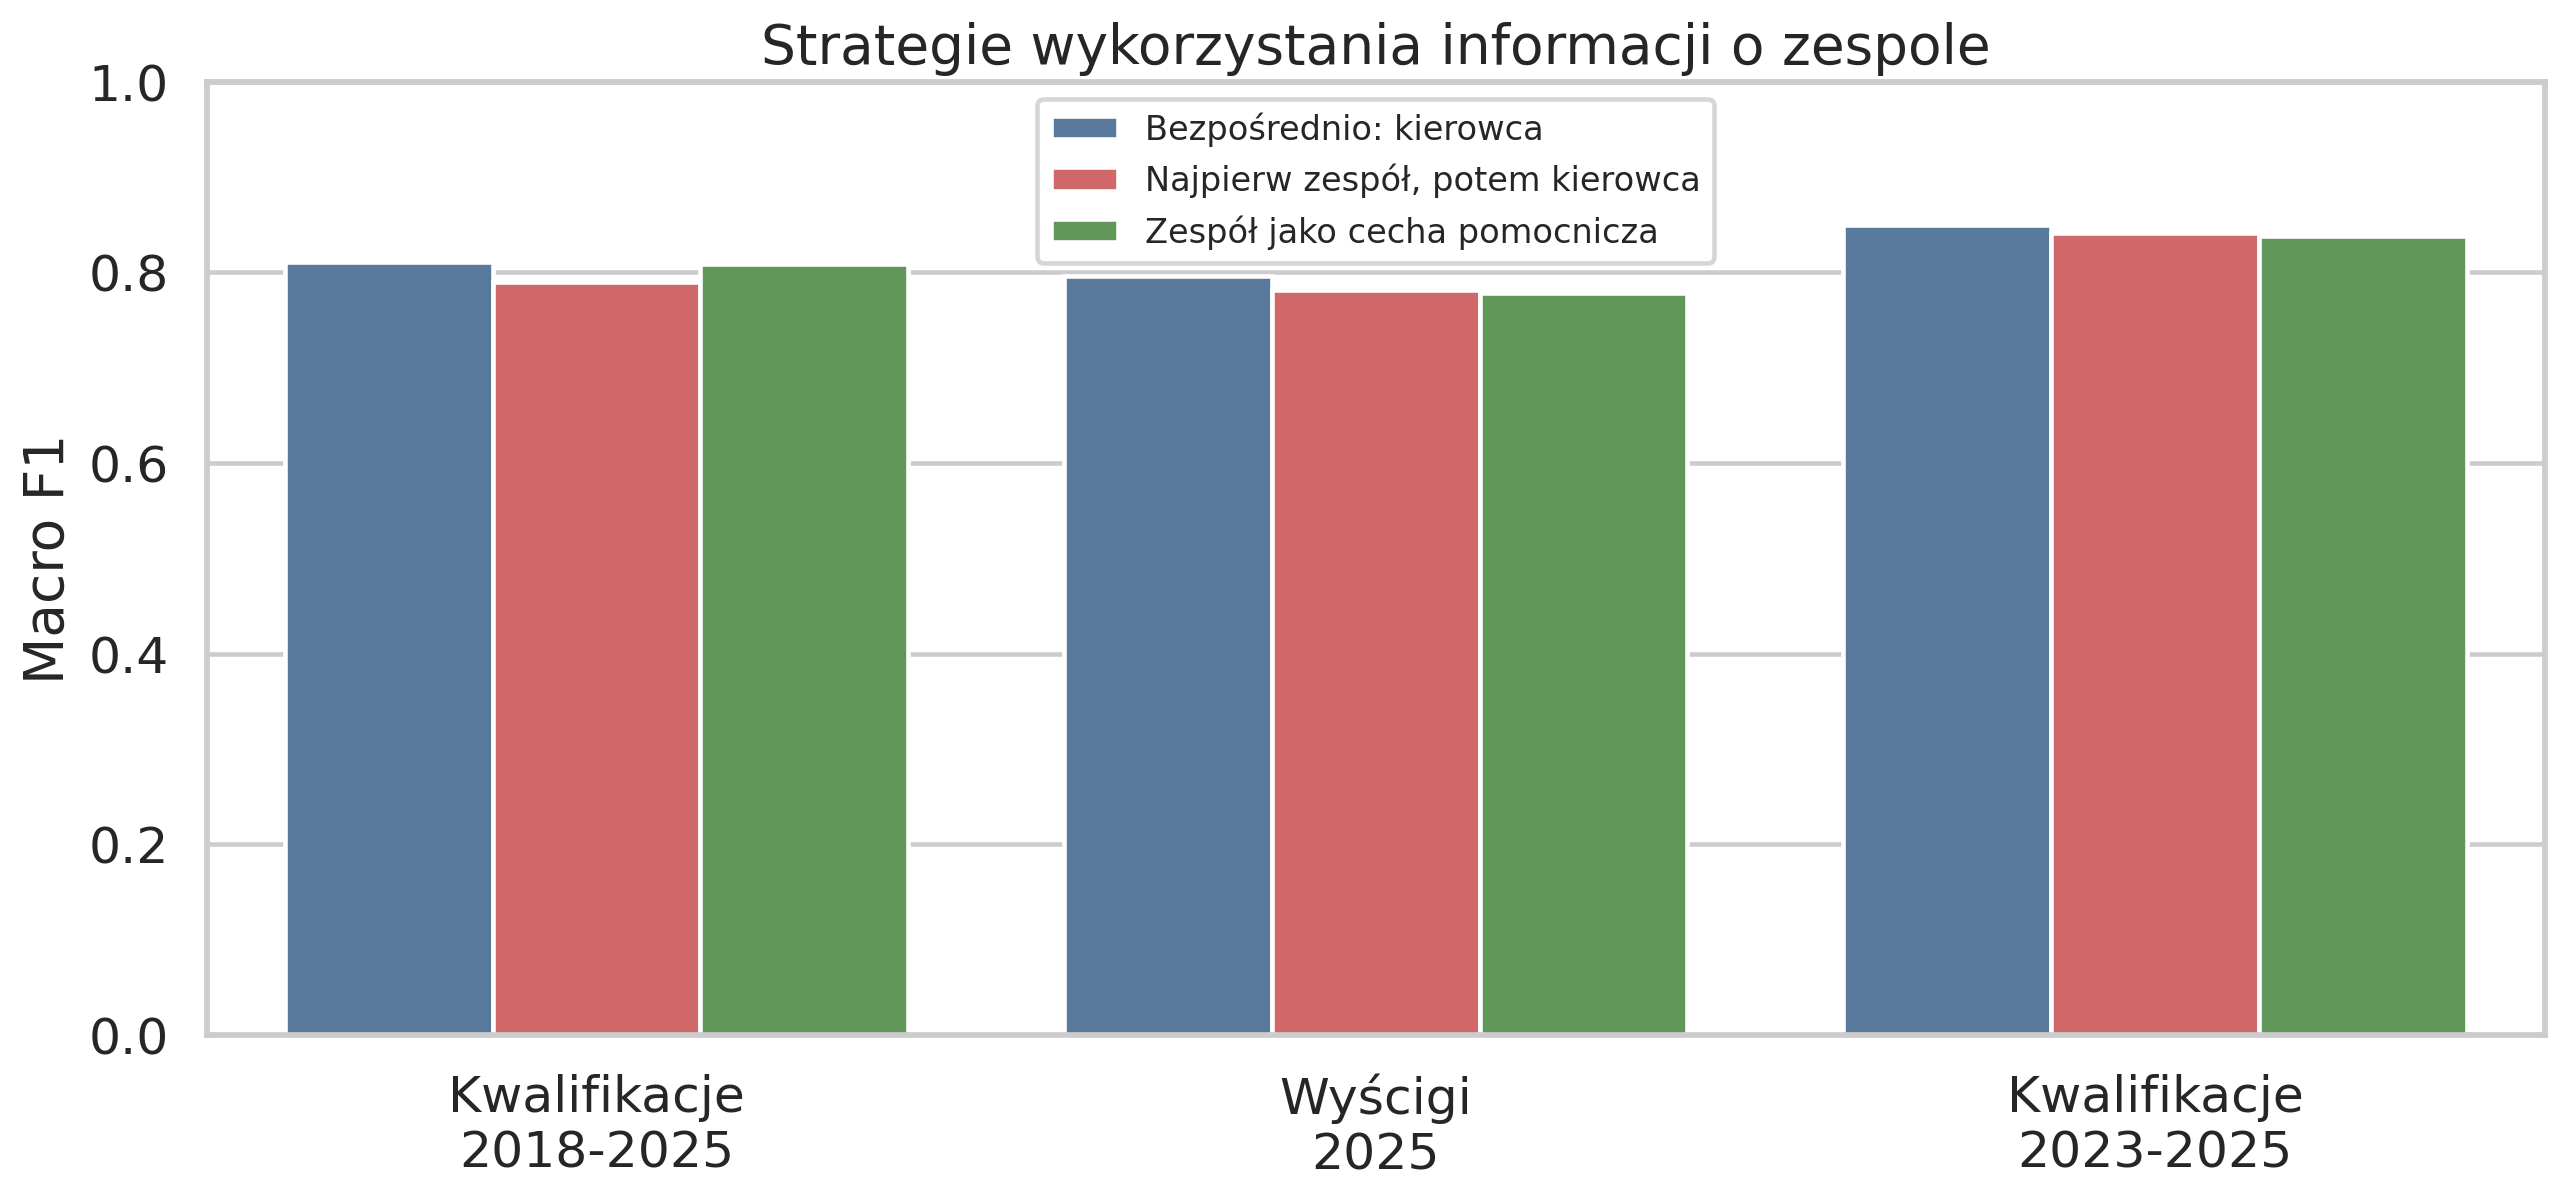
\includegraphics[width=0.90\textwidth]{08_hierarchical_team_aware_comparison.png}
\caption{Porównanie strategii wykorzystania informacji o zespole.}
\label{fig:team-aware}
\end{figure}
\FloatBarrier

Modele wykorzystujące informację o zespole nie poprawiły stabilnie bezpośredniej predykcji kierowcy. Oznacza to, że predykcja zespołu jest ważna głównie jako analiza kontrolna i interpretacyjna, a nie jako najlepsza ścieżka modelowania kierowcy.

\begin{table}[H]
\centering
\small
\begin{tabular}{lccc}
\toprule
Setup & Model bezpośredni & Model hierarchiczny & Model team-aware \\
\midrule
Kwalifikacje 2023--2025 & 0.8451 & 0.8411 & 0.8381 \\
Kwalifikacje 2018--2025 & 0.8059 & 0.7890 & 0.8086 \\
Wyścigi 2025 & 0.7965 & 0.7820 & 0.7786 \\
\bottomrule
\end{tabular}
\caption{Porównanie macro F1 dla regresji logistycznej: model bezpośredni, hierarchiczny i team-aware.}
\label{tab:hierarchical-team-aware}
\end{table}

Z tabeli~\ref{tab:hierarchical-team-aware} wynika, że predykcja zespołu jako etap pomocniczy nie była uniwersalnie lepszą strategią. W długim setupie kwalifikacyjnym wariant team-aware minimalnie poprawił regresję logistyczną, ale w pozostałych setupach pogarszał wynik. Analiza zespołowa pełni więc funkcję kontroli biasu i narzędzia interpretacyjnego, a nie finalnej metody identyfikacji kierowcy.

\section{Test w tym samym zespole}

Najważniejszym testem kontrolnym jest rozróżnianie kierowców w tym samym zespole. Jeżeli model potrafi rozróżnić kierowców jadących tym samym samochodem, to sygnał kierowcy nie może być wyjaśniony wyłącznie charakterystyką zespołu.

\begin{table}[H]
\centering
\small
\begin{tabular}{lccc}
\toprule
Przypadek & Liczba okrążeń & Kierowcy & Macro F1 \\
\midrule
Ferrari, kwalifikacje 2023--2024 & 87 & LEC vs SAI & 0.8612 \\
Ferrari, wyścigi 2025 & 1742 & HAM vs LEC & 0.8820 \\
Ferrari, kwalifikacje 2018--2025 & 219 & LEC/SAI/HAM & 0.7463 \\
\bottomrule
\end{tabular}
\caption{Testy rozróżniania kierowców w tym samym zespole.}
\label{tab:same-team-tests}
\end{table}

\begin{figure}[H]
\centering
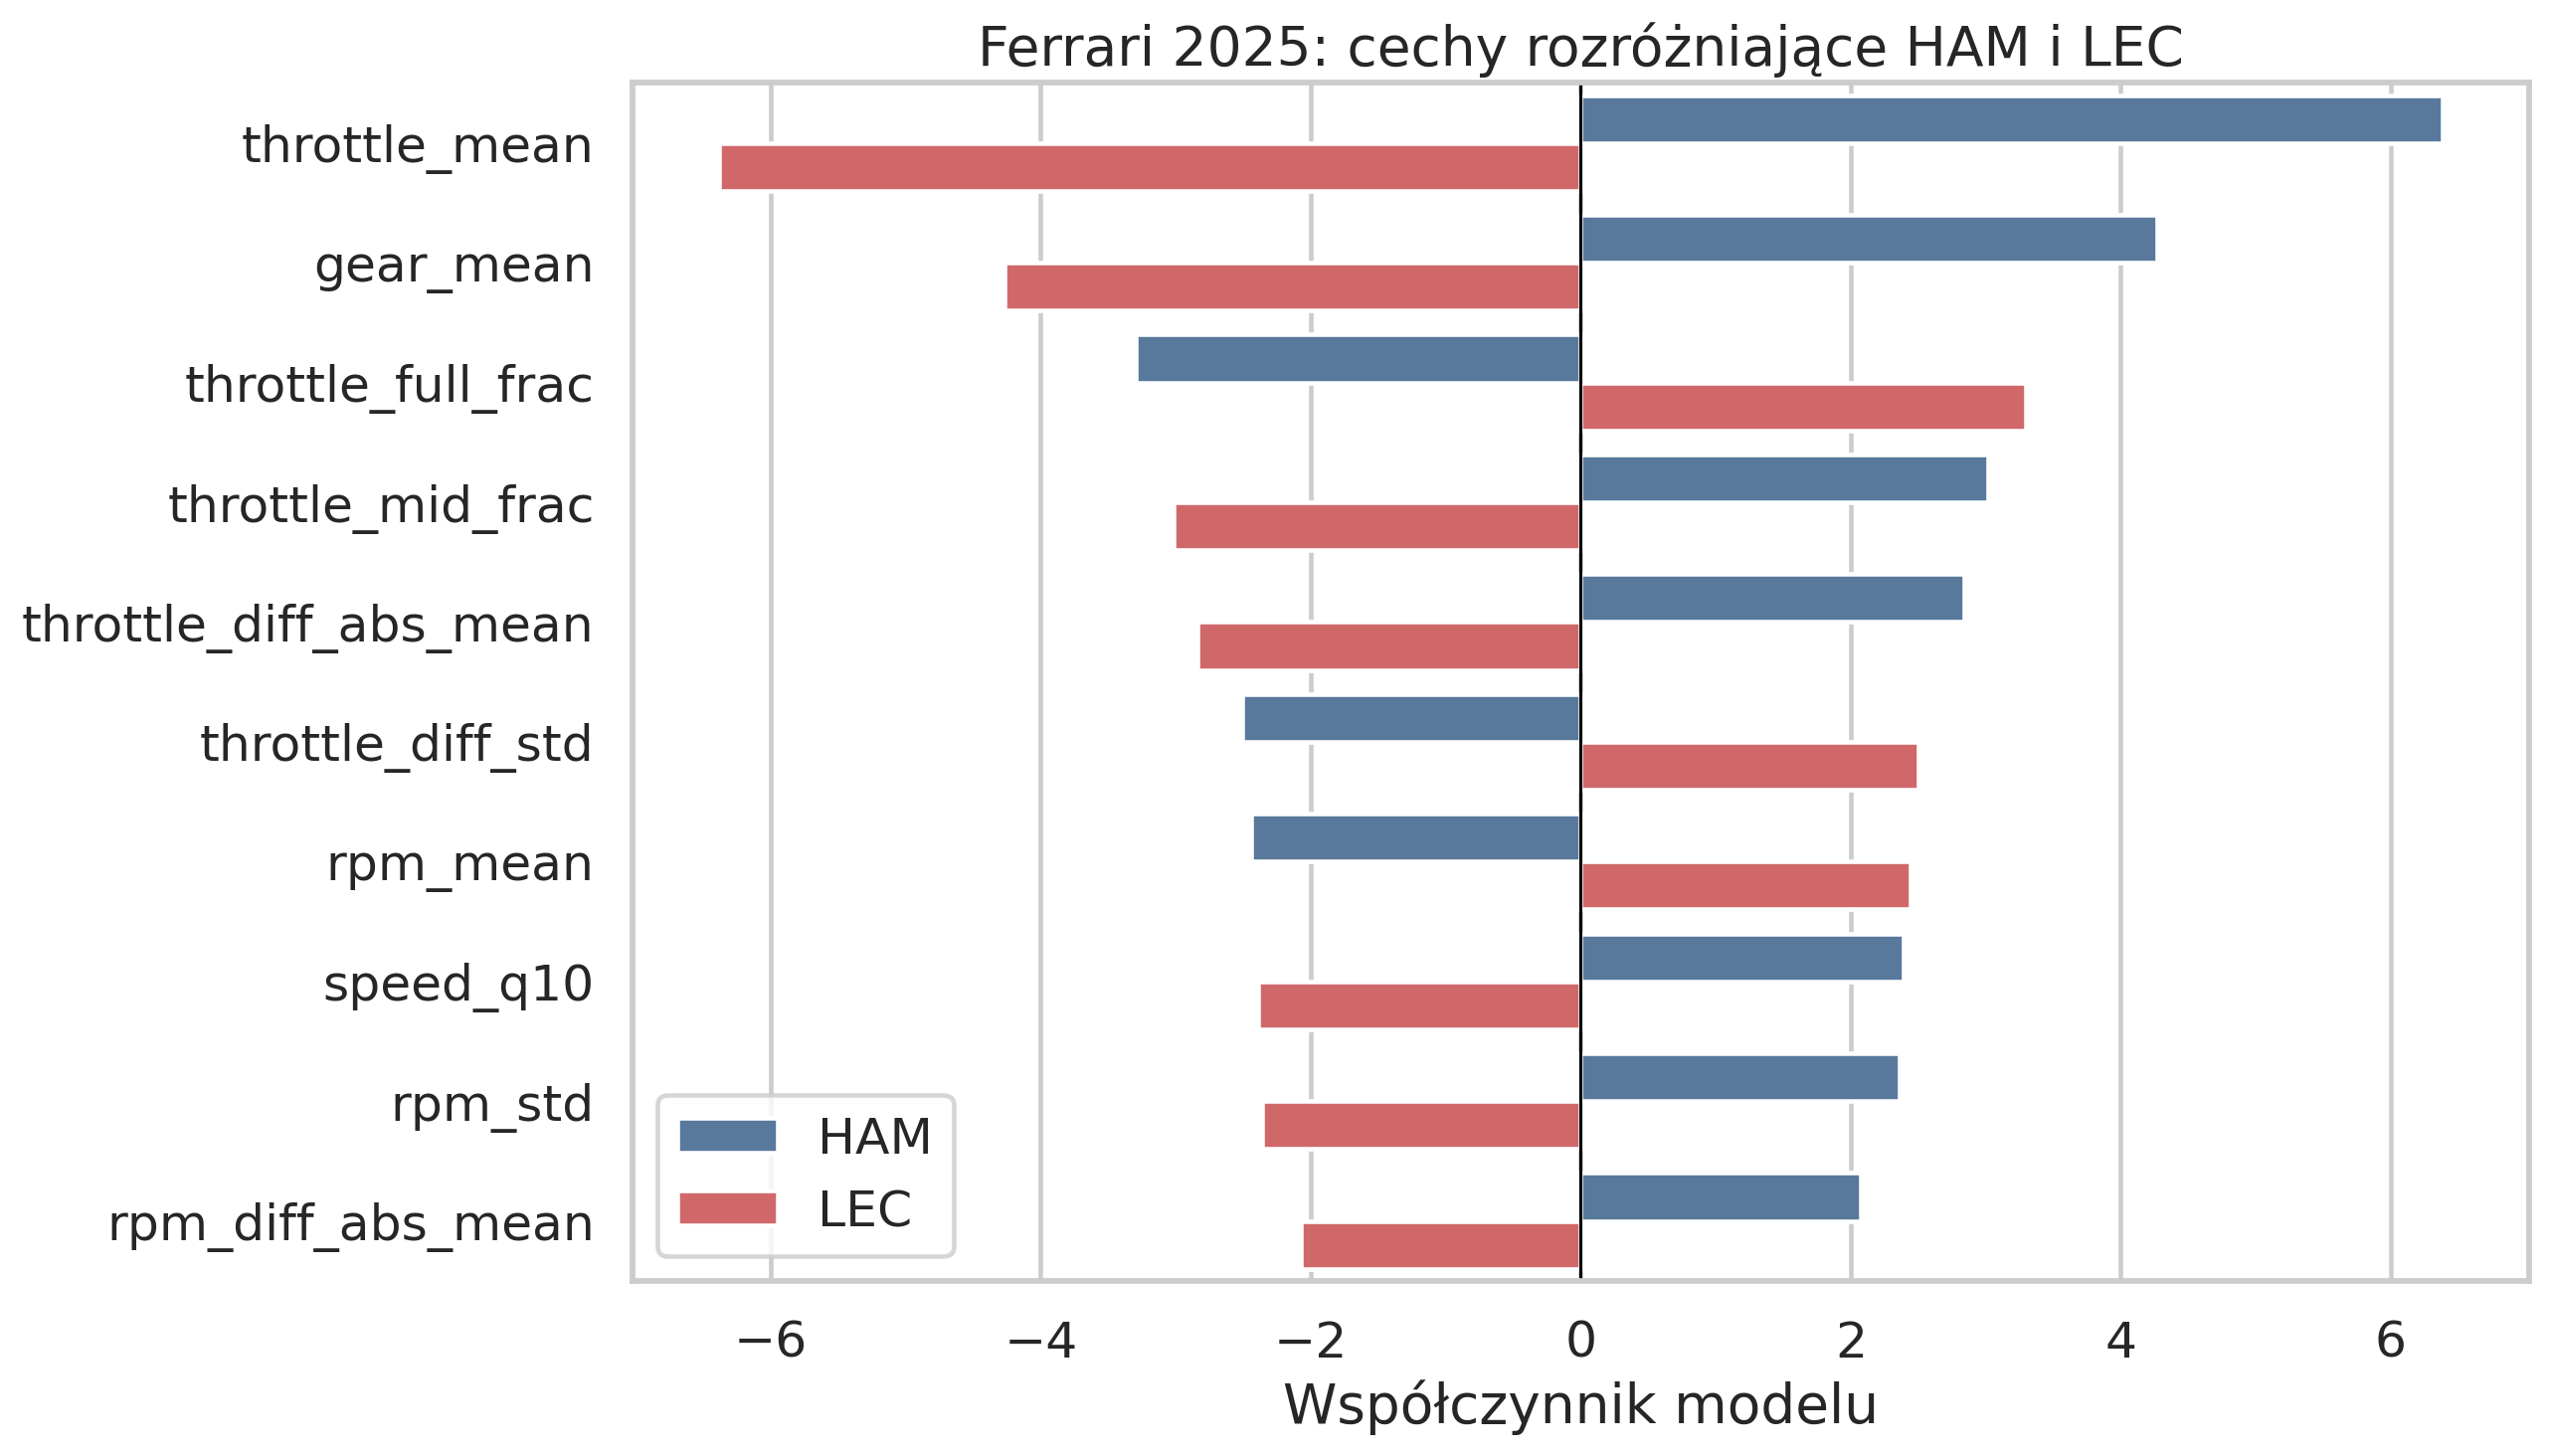
\includegraphics[width=0.90\textwidth]{09_same_team_ham_lec_feature_importance.png}
\caption{Ferrari 2025: cechy rozróżniające Hamiltona i Leclerca.}
\label{fig:same-team}
\end{figure}

Przykład Ferrari 2025 pokazuje, że model znajduje różnice między Hamiltonem i Leclerkiem mimo jazdy w tym samym zespole. Wśród ważnych cech pojawiały się między innymi cechy przepustnicy, średniego biegu, dynamiki gazu, prędkości oraz obrotów. Jest to istotny argument, że w telemetrii pozostaje indywidualny sygnał kierowcy, nawet jeżeli samochód i zespół mają własny wyraźny wpływ na dane.

Taki test jest odpowiednikiem kontroli zmiennej zakłócającej. Skoro samochód i zespół mogą wpływać na telemetrię, to rozróżnianie kierowców w tym samym zespole jest silniejszym argumentem niż sama klasyfikacja kierowców z różnych zespołów. W tym sensie wyniki są zgodne z pracami o identyfikacji kierowcy z danych pojazdu, ale dodają kontrolę specyficzną dla Formuły 1.

\chapter{Badanie 3: Stabilność stylu po zmianie zespołu}

\section{Motywacja}

Trzecie badanie rozszerza wcześniejsze wyniki. Skoro model potrafi rozpoznać kierowcę, a jednocześnie wiadomo, że zespół wpływa na sygnał, naturalnym pytaniem jest to, czy elementy stylu kierowcy są częściowo stabilne po zmianie samochodu.

Nie zakładano pełnej niezależności stylu kierowcy od auta. Sprawdzono raczej, czy mimo zmiany zespołu pewne profile telemetryczne pozostają podobne.

\section{Metoda}

Porównano kierowców, którzy w analizowanym okresie zmieniali zespoły. Cechy były normalizowane względem sesji, aby ograniczyć wpływ toru i warunków. Następnie dla każdego kierowcy porównano profile \emph{kierowca--zespół}.

W głównej części pokazano wybrane przypadki, natomiast pełne wyniki powinny zostać umieszczone w dodatku lub repozytorium. Ogranicza to ryzyko wybierania wyłącznie przykładów pasujących do tezy.

\section{Wyniki stabilności stylu}

Zbiorcze porównanie stabilności profilu stylu między zespołami przedstawiono na rysunku~\ref{fig:transfer-stability}.

\begin{figure}[H]
\centering
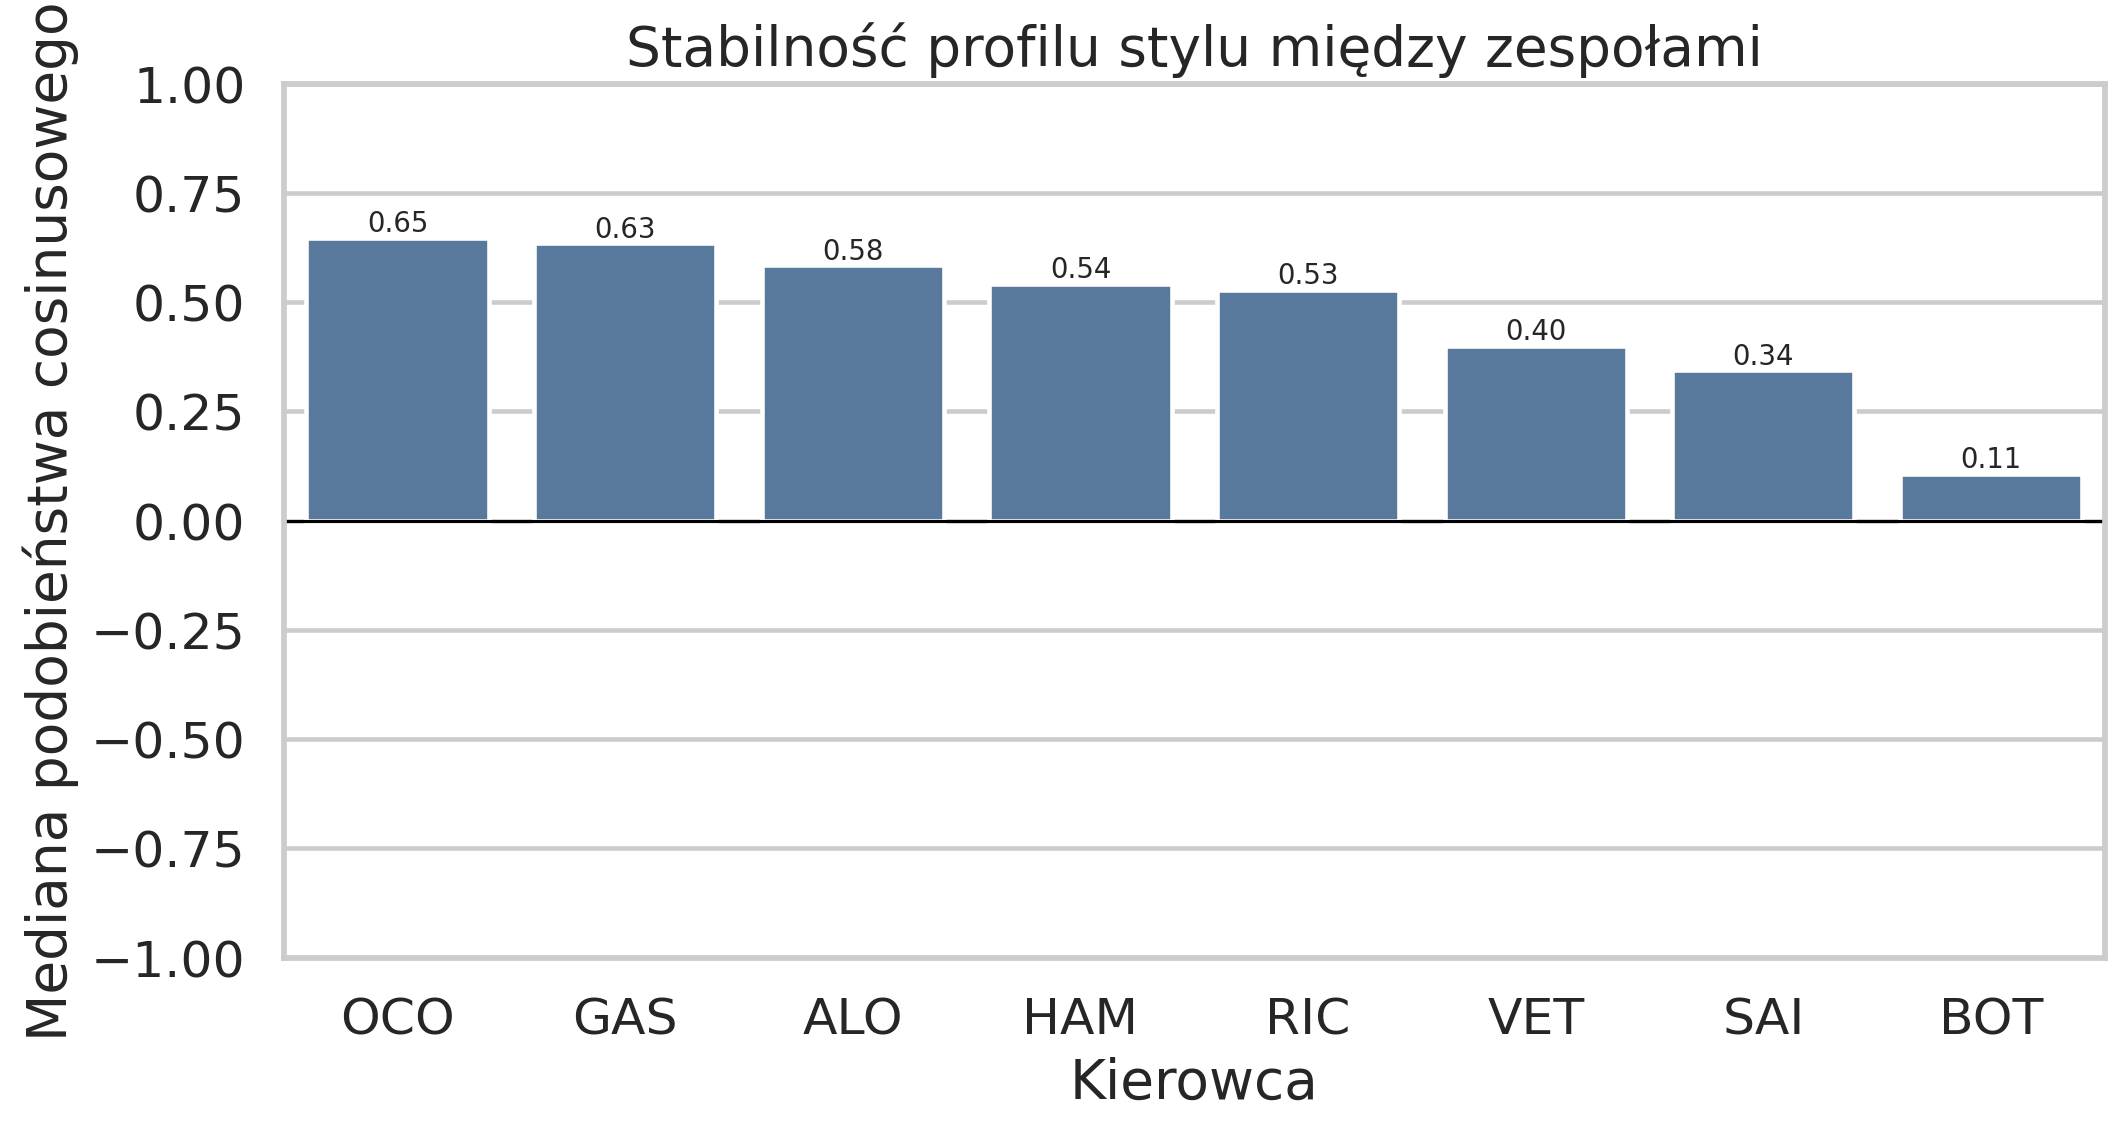
\includegraphics[width=0.90\textwidth]{19_driver_style_transfer_stability_summary.png}
\caption{Stabilność profilu stylu między zespołami dla kierowców zmieniających zespół.}
\label{fig:transfer-stability}
\end{figure}

Rysunek pokazuje, że stabilność profilu nie jest jednorodna: u części kierowców podobieństwo między zespołami pozostaje wyraźne, a u innych jest znacznie słabsze.

\begin{table}[H]
\centering
\small
\begin{tabular}{lccc}
\toprule
Kierowca & Liczba par zespołów & Mediana podobieństwa & Interpretacja \\
\midrule
OCO & 10 & 0.648 & mocny przykład stabilności \\
GAS & 6 & 0.634 & mocny przykład stabilności \\
ALO & 3 & 0.584 & mocny przykład stabilności \\
RIC & 10 & 0.528 & częściowy przykład \\
SAI & 6 & 0.345 & kontrprzykład \\
BOT & 3 & 0.107 & kontrprzykład \\
\bottomrule
\end{tabular}
\caption{Wybrane przypadki stabilności stylu po zmianie zespołu.}
\label{tab:transfer-cases}
\end{table}

\begin{figure}[H]
\centering
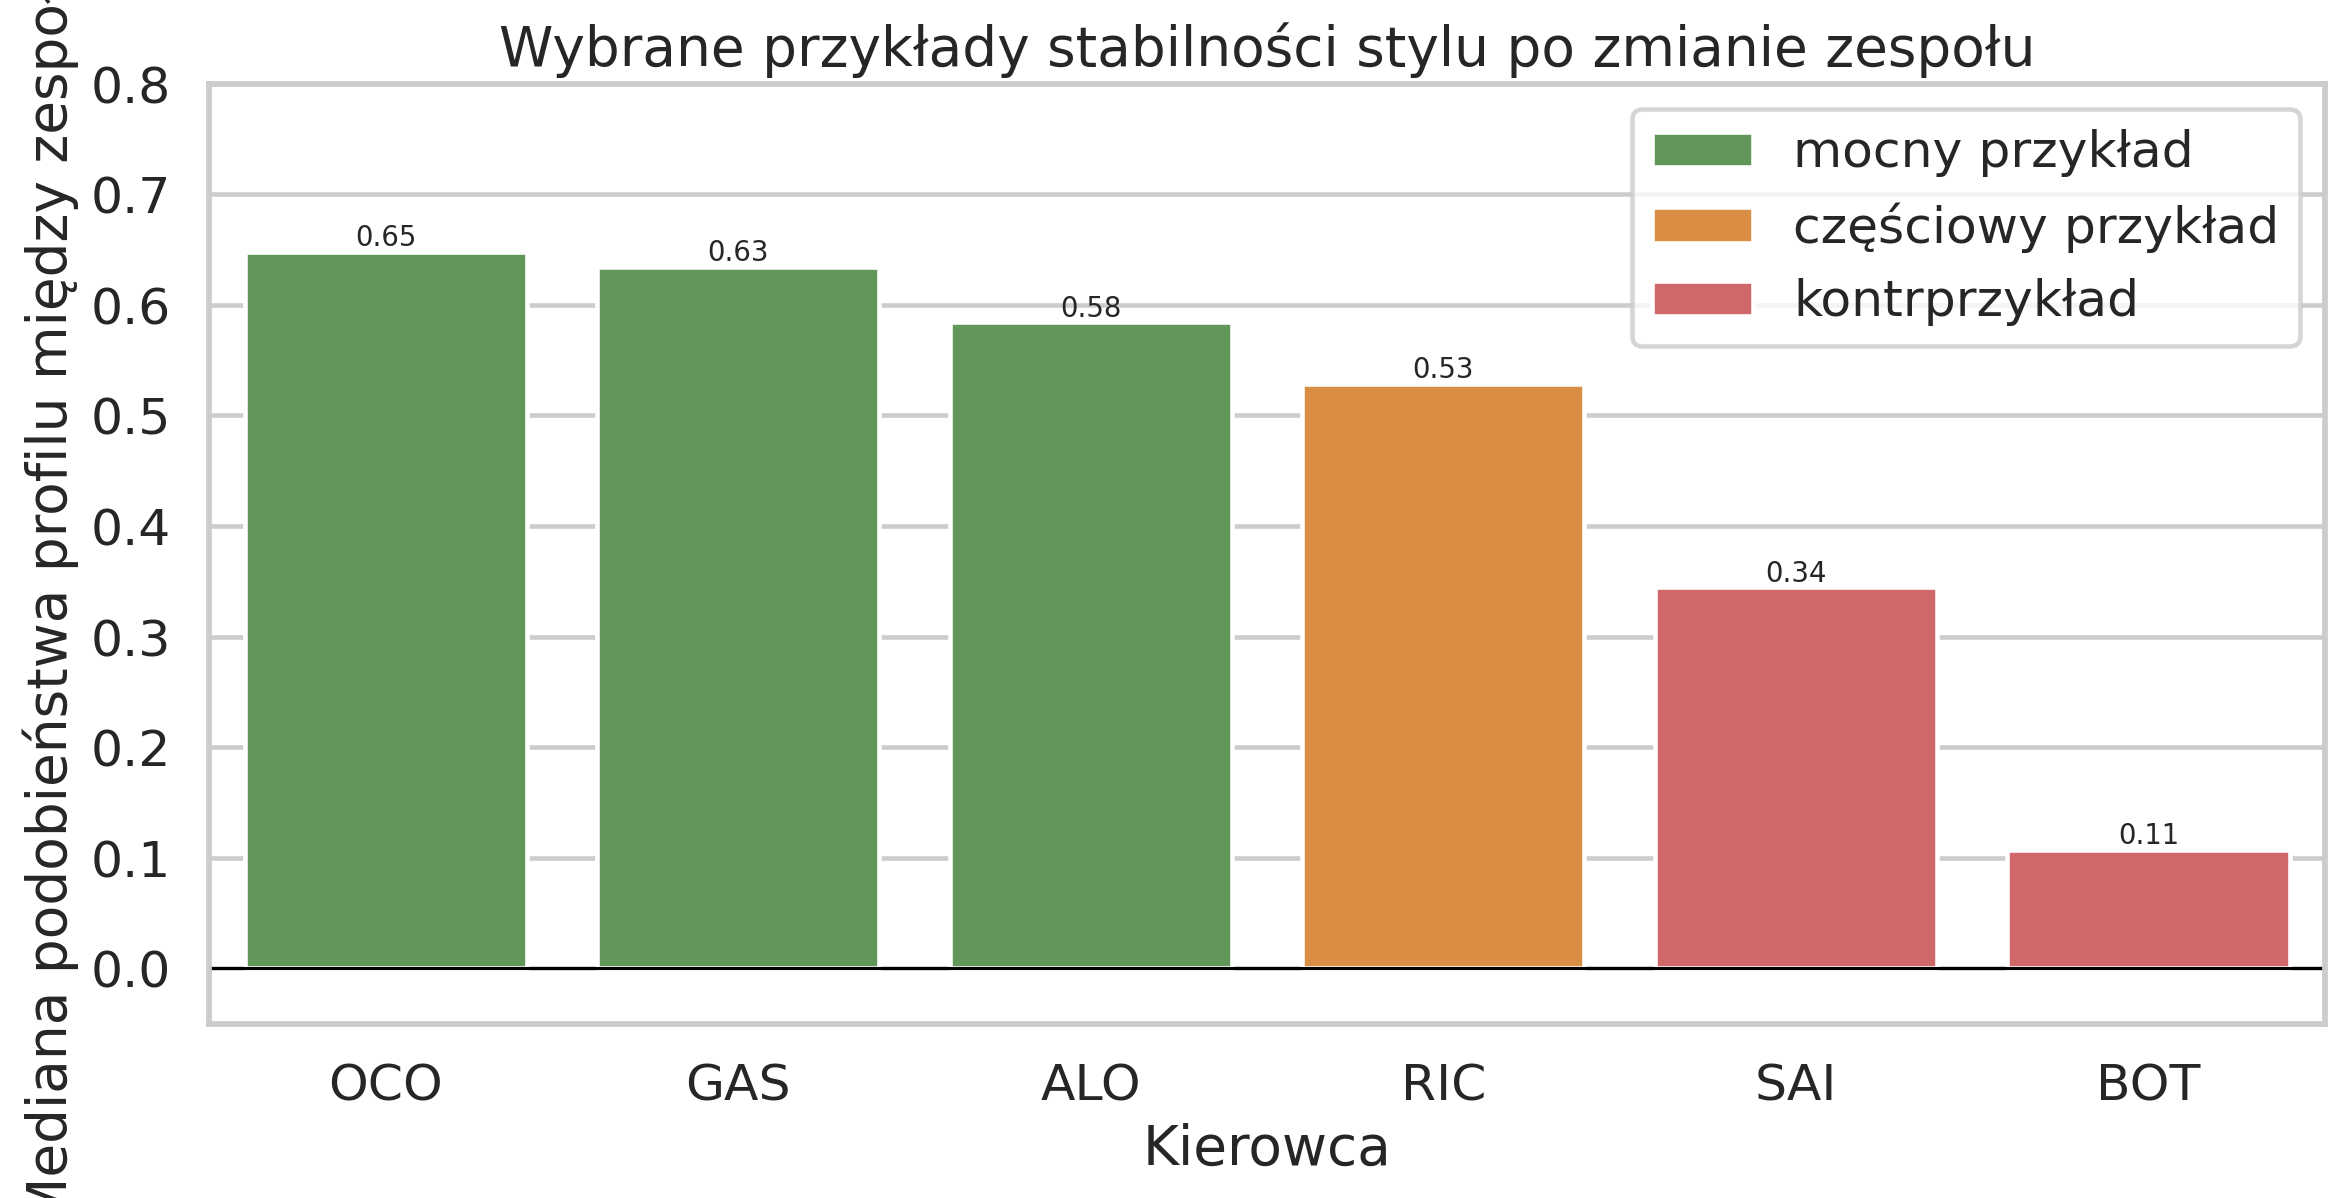
\includegraphics[width=0.90\textwidth]{23_selected_driver_transfer_case_studies.png}
\caption{Wybrane przykłady stabilności i niestabilności stylu po zmianie zespołu.}
\label{fig:selected-transfer}
\end{figure}
\FloatBarrier

Wyniki sugerują, że u części kierowców profil stylu pozostaje częściowo stabilny po zmianie zespołu. Najmocniejsze przykłady w tej analizie to Ocon, Gasly i Alonso. Ricciardo jest przypadkiem częściowym: część jego profili między zespołami jest podobna, ale nie wszystkie. Sainz i Bottas pokazują natomiast, że samochód i kontekst mogą znacząco zmienić profil telemetryczny.

\section{Synteza wyników}

Powiązanie kolejnych etapów analizy przedstawiono na rysunku~\ref{fig:research-arc}.

\begin{figure}[H]
\centering
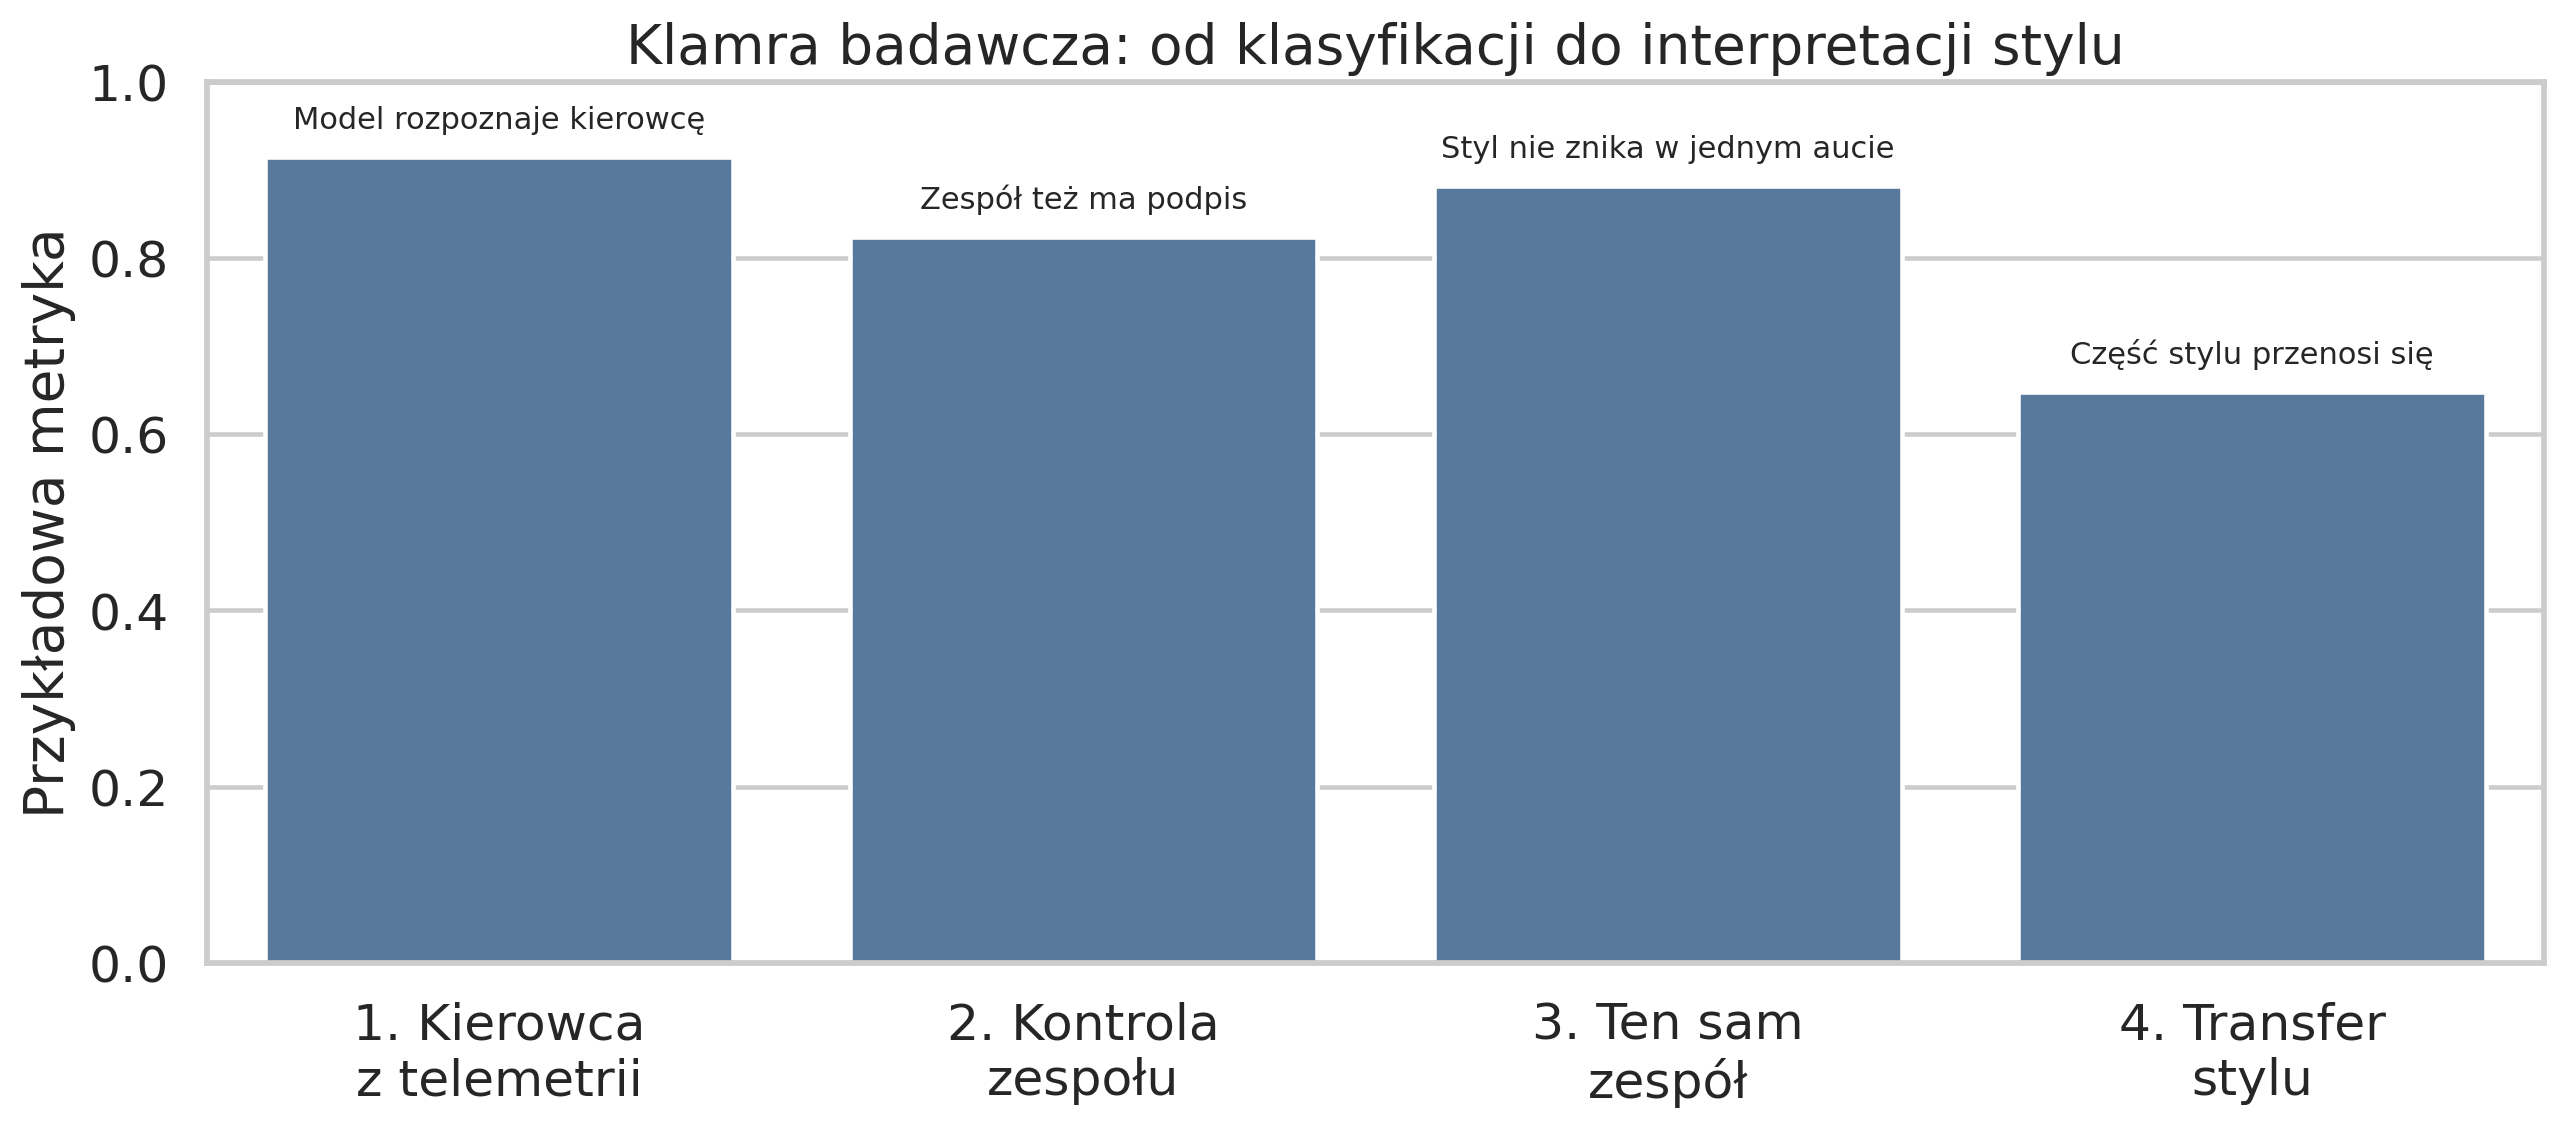
\includegraphics[width=0.90\textwidth]{22_thesis_research_arc.png}
\caption{Proces badawczy: od klasyfikacji do interpretacji stylu.}
\label{fig:research-arc}
\end{figure}

Proces badawczy prowadzi od klasyfikacji do interpretacji:

\begin{enumerate}
    \item modele potrafią rozpoznać kierowcę na podstawie telemetrii;
    \item zespół również ma podpis telemetryczny, więc konieczna jest kontrola biasu;
    \item testy w tym samym zespole pokazują, że indywidualny sygnał kierowcy nie znika;
    \item wybrane przypadki transferu między zespołami sugerują, że część stylu może być stabilna mimo zmiany samochodu.
\end{enumerate}

\chapter{Podsumowanie i dalsze prace}

Praca pokazuje, że identyfikacja kierowcy Formuły 1 na podstawie telemetrii jest możliwa. Modele osiągały wyniki wyraźnie lepsze od losowych we wszystkich trzech setupach eksperymentalnych, a najlepsze rezultaty uzyskiwały modele sekwencyjne i hybrydowe. Regresja logistyczna pozostała natomiast ważnym punktem odniesienia, ponieważ pozwalała nie tylko klasyfikować kierowców, ale również interpretować cechy związane z decyzją modelu.

Najważniejszym wnioskiem nie jest sama skuteczność klasyfikacji, lecz to, że telemetria zawiera informacje opisujące sposób pokonywania okrążenia. Różnice między kierowcami były widoczne zarówno w ręcznie zdefiniowanych cechach, jak i w przebiegach sekwencyjnych. Modele wykorzystywały między innymi informacje związane z prędkością, pracą gazu, hamowaniem, biegami, obrotami silnika i dynamiką sygnałów. Oznacza to, że końcowy czas okrążenia nie wyczerpuje opisu jazdy kierowcy.

Ważnym rozszerzeniem była analiza wpływu zespołu i samochodu. Zespół również ma własny profil telemetryczny, dlatego klasyfikacji kierowcy nie można interpretować w oderwaniu od samochodu. Testy w obrębie tego samego zespołu oraz analiza kierowców zmieniających zespoły sugerują jednak, że indywidualny profil kierowcy nie znika całkowicie. Styl jazdy nie jest więc ani całkowicie niezależny od samochodu, ani całkowicie przez samochód determinowany.

Zakres wniosków jest ograniczony przez charakter publicznie dostępnych danych. Część obserwowanych różnic można interpretować tylko pośrednio, bez pełnego dostępu do informacji inżynierskich wykorzystywanych przez zespoły. Mimo tego dostępna telemetria okazała się wystarczająca do zbudowania stabilnego procesu badawczego i uzyskania wyników interpretowalnych w kontekście stylu jazdy.

\section{Możliwe dalsze kierunki}

\begin{itemize}
    \item precyzyjne wyrównanie czasowe danych samochodu i pozycji;
    \item segmentacja okrążenia na zakręty i mini-sektory;
    \item analiza stylu kierowcy tor po torze;
    \item wykorzystanie danych OpenF1 jako niezależnego źródła walidacji;
    \item budowa embeddingów stylu kierowcy;
    \item dashboard do porównywania kierowców i zespołów;
    \item analiza transferu kierowcy między zespołami na większej liczbie sezonów.
\end{itemize}

\cleardoublepage
\printbibliography[heading=bibintoc,title={Literatura}]

% Opcjonalnie, jeżeli promotor/uczelnia tego wymaga:
% \listoffigures
% \listoftables

\end{document}
